

%build with
%pdflatex main.tex 2>&/dev/null ; bibtex main 2>&/dev/null ; latexmk -pdf -f -g -bibtex -deps -synctex=1 -interaction=nonstopmode --shell-escape main.tex


%TC:macro \lstinline [xx]
%TC:envir lstlisting [] xall
\documentclass[12pt]{report}
\usepackage[paper=A4,pagesize]{typearea}
\usepackage{afterpage}
\usepackage[utf8]{inputenc}
\usepackage{graphicx}
\graphicspath{ {images/} }
\usepackage[hidelinks]{hyperref}
\usepackage[final]{pdfpages}
\usepackage{caption}
\usepackage{subcaption}
\usepackage[a4paper,width=175mm,top=25mm,bottom=25mm]{geometry}
\usepackage{fancyhdr}
\usepackage{enumitem}
\usepackage{float}
\usepackage{longtable}
\usepackage{amsmath}
\usepackage{xcolor}
\usepackage{amsmath}
\usepackage{array}
\usepackage{moreverb}
\usepackage{dirtree}
\usepackage{changepage}
\usepackage{tikz}
\usepackage{lmodern,textcomp}
\usepackage[printonlyused,withpage]{acronym}
\pagestyle{fancy}
%puts chapter name in footer
\renewcommand{\chaptermark}[1]{\markboth{#1}{#1}}
\fancyhead{}
\fancyhead[R]{Brain Connectivity Mapping Using Anatomical MRI}
\fancyfoot{}
\fancyfoot[R]{\thepage}
\fancyfoot[L]{\leftmark}
\renewcommand{\headrulewidth}{0.4pt}
\renewcommand{\footrulewidth}{0.4pt}
\usepackage{titlesec}
%hides chapter text
\titleformat{\chapter}[display]{\normalfont\bfseries}{}{0pt}{\Huge}
\titlespacing*{\chapter}{0pt}{-10pt}{30pt}
%paragraph indent
\setlength{\parindent}{12pt}
%paragraph spacing
\setlength{\parskip}{3pt}
%makes the numbering of the subsubsection alphabetical
\renewcommand{\thesubsubsection}{\thesubsection.\alph{subsubsection}}
\setcounter{secnumdepth}{4}
\setcounter{tocdepth}{2}
%creates left and right aligned table columns
\newcolumntype{R}[1]{>{\raggedleft\arraybackslash}p{#1}}
\newcolumntype{L}[1]{>{\raggedright\arraybackslash}p{#1}}
%code snippets
\usepackage{listings}
\usepackage{color}
\definecolor{dkgreen}{rgb}{0,0.6,0}
\definecolor{gray}{rgb}{0.5,0.5,0.5}
\definecolor{mauve}{rgb}{0.58,0,0.82}
\lstset{frame=tb,
  language=python,
  morekeywords={as},
  aboveskip=3mm,
  belowskip=3mm,
  showstringspaces=false,
  columns=fixed,
  basicstyle={\small\ttfamily},
  numbers=left,
  numberstyle=\tiny\color{gray},
  keywordstyle=\color{blue},
  commentstyle=\color{dkgreen},
  stringstyle=\color{mauve},
  breaklines=false,
  breakatwhitespace=true,
  tabsize=2
}
%references
\usepackage{csquotes}
\usepackage[utf8]{inputenc}
\usepackage[english]{babel}
\usepackage[backend=bibtex,sorting=none]{biblatex}
\addbibresource{references.bib}
%cite with clickable link wrapping some text as well
\newcommand{\citelink}[2]{\hyperlink{cite.\therefsection @#1}{#2} \cite{#1}}
%cite with clickable link wrapping some text as well
\newcommand{\reflink}[2]{\hyperref[#1]{#2} \ref{#1}}
%pdf details
\hypersetup{
  pdftitle={Predicting Brain Connectivity Mapping Using Radiomics Features in Anatomical MRI},
  pdfauthor={Levente Zsolt Nagy},
  pdfsubject={Medical Imaging},
  pdfkeywords={dMRI,MRI,DTI,magnetic resonance imaging,tractography,brain connectivity,radiomics,medical imaging},
  pdfcreator={Levente Zsolt Nagy},
}
%no break longtable hline
\makeatletter
\def\nobreakhline{%
  \noalign{\ifnum0=`}\fi
    \penalty\@M
    \futurelet\@let@token\LT@@nobreakhline}
\def\LT@@nobreakhline{%
  \ifx\@let@token\hline
    \global\let\@gtempa\@gobble
    \gdef\LT@sep{\penalty\@M\vskip\doublerulesep}
  \else
    \global\let\@gtempa\@empty
    \gdef\LT@sep{\penalty\@M\vskip-\arrayrulewidth}
  \fi
  \ifnum0=`{\fi}%
  \multispan\LT@cols
     \unskip\leaders\hrule\@height\arrayrulewidth\hfill\cr
  \noalign{\LT@sep}%
  \multispan\LT@cols
     \unskip\leaders\hrule\@height\arrayrulewidth\hfill\cr
  \noalign{\penalty\@M}%
  \@gtempa}
\makeatother
%title and author and date
\title{Predicting Brain Connectivity Mapping Using Radiomics Features in Anatomical MRI}
\author{Levente Zsolt Nagy}
\date{2024-12-15}
%word count
\immediate\write18{
  echo "Number of Words: " > wc.tex &&
  texcount main.tex -sum -1 -merge >> wc.tex &&
  echo "\\\\Number of Characters: " >> wc.tex &&
  texcount main.tex -sum -1 -merge -char >> wc.tex
}
%actual doc
\begin{document}
%TC:ignore
\begin{titlepage}
    \begin{center}
        \begingroup
          \let\clearpage\relax

          
\includegraphics[width=1\textwidth]{banner.png}
          \vfill
          \LARGE
          \begin{center}
          \textbf{\MakeUppercase{Predicting Brain Connectivity Mapping Using Radiomics Features in Anatomical MRI}}
          \end{center}
          \vfill
          \large
          \textbf{\MakeUppercase{Levente Zsolt Nagy}}
          \vfill
          \normalsize
          \textbf{Thesis supervisor}\\
          \MakeUppercase{Alfredo Vellido Alcacena} (Department of Computer Science)\\
          \hfill\\
          \textbf{Thesis co-supervisor}\\
          \MakeUppercase{Estela Camara Mancha} (Hospital Universitari de Bellvitge)\\
          \hfill\\
          \textbf{Degree}\\
          Master's Degree in Artificial Intelligence\\
          \hfill\\\hfill\\
          \textbf{Master's thesis}\\
          \hfill\\
          \textbf{School of Engineering}\\
          \textbf{Universitat Rovira i Virgili (URV)}\\
          \hfill\\
          \textbf{Faculty of Mathematics}\\
          \textbf{Universitat de Barcelona (UB)}\\
          \hfill\\
          \textbf{Barcelona School of Informatics (FIB)}\\
          \textbf{Universitat Politècnica de Catalunya (UPC) - BarcelonaTech}\\
%           \Huge
%           \textbf{Enhancing Brain Connectivity Mapping:\\
%             A Radiomics Approach to\\
%             Diffusion MRI Tractography}

%           \vspace{0.1cm}
%           \LARGE
%           Medical Imaging

%           \vspace{1.0cm}

%           Levente Zsolt Nagy\\
%           \vspace{1.0cm}
%           \Large
%           \emph{Supervisors}\\
%           Estela Camara Mancha\\
%           Alfredo Vellido Alcacena\\
%           \LARGE

%           \vfill

%           A thesis presented for the degree of\\
%           Master in Artificial Intelligence

%           \vspace{1.0cm}
%           \includegraphics[width=0.37\textwidth]{upc.png}\\
%           \vspace{0.2cm}
%           \hspace{7px}\includegraphics[width=0.37\textwidth]{ub.png}\\
%           \vspace{0.2cm}
%           \includegraphics[width=0.37\textwidth]{bellvitge.png}\\
%           \vspace{1.0cm}

%           \Large
%           Universitat Politècnica de Catalunya\\
%           Universitat de Barcelona\\
%           Hospital Universitari de Bellvitge\\
%           Spain\\
%           2024-12-15\\
%           Number of Words: 
681
\\Number of Characters: 
3682


        \endgroup
    \end{center}
\end{titlepage}
%TC:endignore
\thispagestyle{plain}
\begin{center}
    \Large
    \textbf{Abstract}
\end{center}
\textit{Anatomical magnetic resonance imaging (MRI), such as T1 and T2 weighted images, are commonly used to distinguish brain tissue types. Diffusion tensor imaging (DTI), a more specialized MRI technique, enables the mapping of white matter and the study of structural connectivity through metrics like fractional anisotropy (FA) and mean diffusivity (MD). However, DTI acquisition is time intensive and often excluded from standard clinical protocols.}\par
\textit{This study introduces a method to synthesize FA and MD images from widely available T1 and T2 weighted anatomical scans, reducing dependence on resource intensive DTI acquisition.}\par
\textit{Radiomics, a rapidly evolving field, focuses on extracting quantitative features from medical imaging, to identify biomarkers associated with clinical labels. It is a well established tool in oncology, particularly for tumor segmentation. Fully convolutional neural networks (FCNNs) are also employed for similar tasks, such as deriving clinical labels for tumor segmentation. However, their reliance on computationally intensive 3D convolutions often necessitates the use of 2D slices from 3D volumes, limiting their feasibility.}\par
\textit{We present a hybrid approach that combines the strengths of radiomics and neural networks. Specifically, we use a feedforward neural network (FNN) as a classification or regression head applied to radiomic features, preserving 3D spatial information during feature extraction while reducing the computational demands of 3D convolutions. This neural network head, akin to fully connected layers in traditional convolutional neural networks (CNNs), offers significant flexibility.}\par
\textit{Our experiments are limited to the basal ganglia, a crucial region involved in brain structure and function that is significantly impacted by neurodegeneration in Huntington’s disease (HD). The inclusion of HD patients allows for assessing the method's reliability and robustness. Additionally, we explore the potential of using the T1/T2 ratio as an input image, which has been proposed in recent studies, as a proxy for the myelin content of the brain. Since myelin plays a role in how DTI functions, the T1/T2 ratio may enhance model performance, effectively bridging anatomical MRI and DTI.}\par
\textit{The results indicate strong performance, with Pearson correlations of 85\% for FA and 95\% for MD predictions. While the correlation decreases significantly for FA and moderately for MD in HD patients, the model’s performance remains consistent when both healthy controls and patients are analyzed together. These findings underscore the promise of our hybrid approach for synthesizing structural connectivity images and improving accessibility to diffusion metrics.}
%TC:ignore
\tableofcontents
\chapter*{List of Notations \& Abbreviations}
\begin{acronym}\itemsep-6pt
  \acro{DTI}{Diffusion Tensor Imaging}
  \acro{MRI}{Magnetic Resonance Imaging}
  \acro{CNS}{central nervous system}
  \acro{dMRI}{diffusion magnetic resonance imaging}
  \acro{FA}{fractional anisotropy}
  \acro{MD}{mean diffusivity}
  \acro{RD}{radial diffusivity}
  \acro{ROI}{region of interest}
  \acro{FMRIB}{functional magnetic resonance imaging of the brain}
  \acro{FNIRT}{\acs{FMRIB}'s nonlinear image registration tool}
  \acro{NIfTI}{neuroimaging informatics technology initiative}
  \acro{FCNN}{fully convolutional neural network}
  \acro{NN}{neural network}
  \acro{CNN}{convolutional neural network}
  \acro{GLCM}{gray level co-occurrence matrix}
  \acro{GLSZM}{gray level size zone matrix}
  \acro{GLRLM}{gray level run length matrix}
  \acro{NGTDM}{neighbouring gray tone difference matrix}
  \acro{GLDM}{gray level dependence matrix}
  \acro{CAP}{CAG Age Product}
  \acro{cUHDRS}{composite Unified Huntington’s Disease Rating Scale}
  \acro{FNN}{feedforward neural network}
  \acro{FSL}{FMRIB software library}
  \acro{UML}{unified modeling language}
\end{acronym}
\listoffigures
\listoftables
%TC:endignore

\chapter{Introduction}
\citelink{basal}{Basal ganglia is a part of the human brain which is group of subcortical nuclei responsible primarily for motor control, as well as other roles such as motor learning, executive functions and behaviors, and emotions.} \citelink{hunting}{Huntington’s disease is a disorder that causes the progressive degeneration of the basal nuclei.}\par

Hospital de Bellvitge provided an excellent dataset of \ac{MRI} and \ac{dMRI} records. This dataset contains 32 control and 37 Huntington patient records of T1 and T1/T2 \ac{MRI} images with isotropic voxels of 1 millimeter resolution and \ac{dMRI} \ac{FA}, \ac{MD} and \ac{RD} images with isotropic voxels of 2 millimeter resolution and 1 second temporal resolution. Furthermore this dataset also contains the mask for the basal ganglia, which will also be referenced as the \ac{ROI}. And taking inspiration from this \citelink{conn}{paper}, masks for the 7 main cortical regions of the brain, which will also be referenced as the target regions: Limbic, Executive, Rostral-Motor, Caudal-Motor, Parietal, Occipital and Temporal are also included in the dataset. Tractography was performed on the \ac{dMRI} images to figure out which parts of the \ac{ROI} are connected to which cortical target, in a similar manner to how it was done in said \citelink{conn}{paper}; where the relative connectivity maps are representing the ratio of the number of streamlines to each cortical target. Furthermore, the raw streamline images are also available, where there are a maximum of 5000 streamlines from each voxel in the \ac{ROI}. The anatomical segmentation of the Basal Ganglia is also available, for the Caudate Putamen and Accumbens. \par

\begin{figure}[H]
\centering
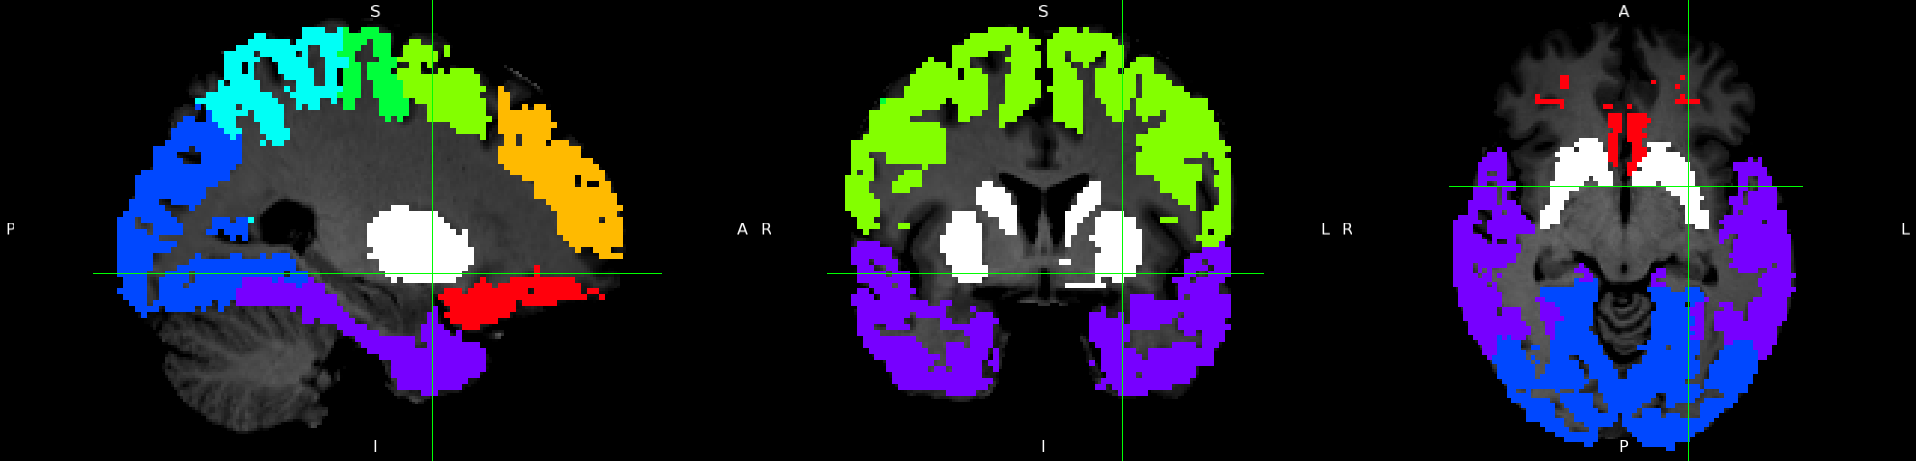
\includegraphics[width=1\textwidth]{rois}
\caption{Basal Ganglia (ROI) \& Cortical Targets}
\label{fig:rois}
\end{figure}

\begin{table}[H]
\centering
\begin{tabular}{|l|l|}
\hline
\textbf{Color} & \textbf{Region} \\ \hline
\begin{tikzpicture}\filldraw[draw=black,fill={rgb,255:red,255;green,255;blue,255}](0,0.15)rectangle(0.25,0.4);\end{tikzpicture} White & Basal Ganglia (ROI) \\ \hline
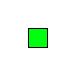
\begin{tikzpicture}\filldraw[draw=black,fill={rgb,255:red,0;green,255;blue,15}](0,0.15)rectangle(0.25,0.4);\end{tikzpicture} Green & Limbic \\ \hline
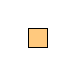
\begin{tikzpicture}\filldraw[draw=black,fill={rgb,255:red,255;green,201;blue,126}](0,0.15)rectangle(0.25,0.4);\end{tikzpicture} Brown & Executive \\ \hline
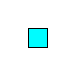
\begin{tikzpicture}\filldraw[draw=black,fill={rgb,255:red,0;green,252;blue,255}](0,0.15)rectangle(0.25,0.4);\end{tikzpicture} Light Blue & Rostral-Motor \\ \hline
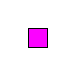
\begin{tikzpicture}\filldraw[draw=black,fill={rgb,255:red,251;green,3;blue,255}](0,0.15)rectangle(0.25,0.4);\end{tikzpicture} Purple & Caudal-Motor \\ \hline
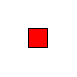
\begin{tikzpicture}\filldraw[draw=black,fill={rgb,255:red,253;green,0;blue,0}](0,0.15)rectangle(0.25,0.4);\end{tikzpicture} Red & Parietal \\ \hline
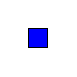
\begin{tikzpicture}\filldraw[draw=black,fill={rgb,255:red,0;green,0;blue,253}](0,0.15)rectangle(0.25,0.4);\end{tikzpicture} Blue & Occipital \\ \hline
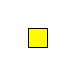
\begin{tikzpicture}\filldraw[draw=black,fill={rgb,255:red,255;green,252;blue,0}](0,0.15)rectangle(0.25,0.4);\end{tikzpicture} Yellow & Temporal \\ \hline
\end{tabular}
\caption{Regions Legend}
\label{tab:reglen}
\end{table}

Furthermore, for both the \ac{ROI} and cortical targets, the dataset distinguishes between the right and left halves of the brain. Thus there are actually 2 \ac{ROI}s and $2 \cdot 7=14$ target regions.

\begin{figure}[H]
\centering
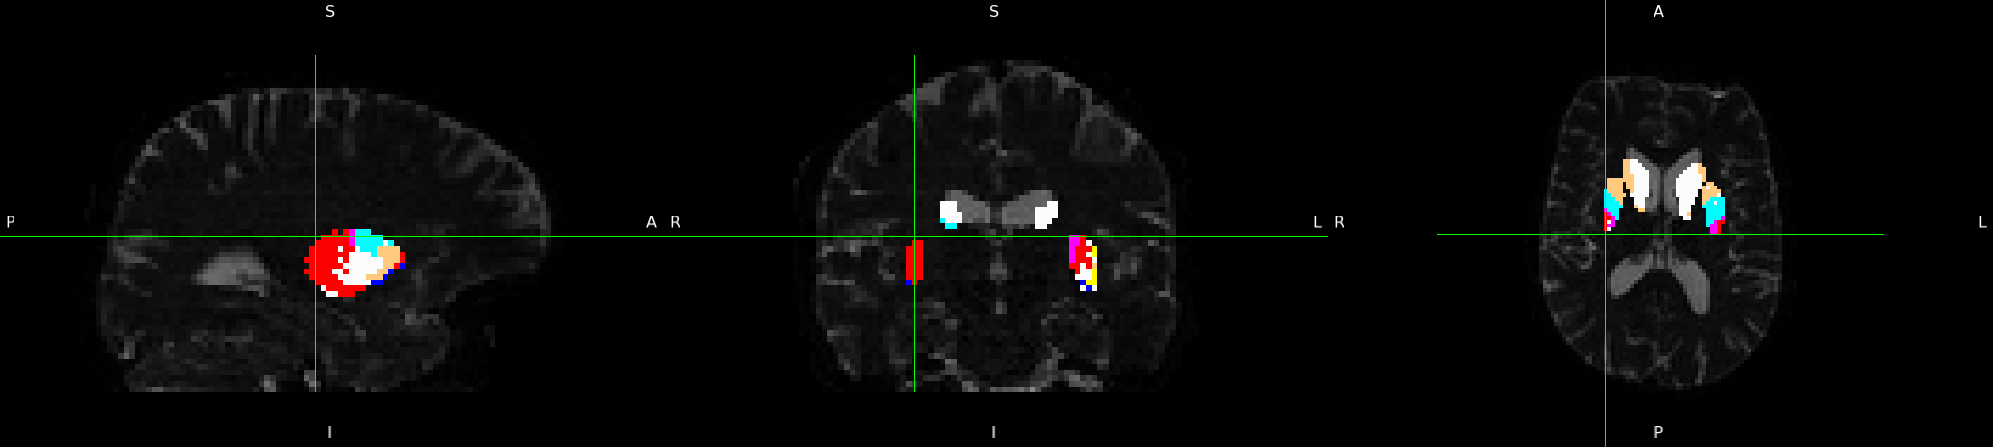
\includegraphics[width=1\textwidth]{conn}
\caption{Connectivity Maps}
\label{fig:conn}
\end{figure}

\section{Objectives}

The end goal is to predict the relative connectivity of the Basal Ganglia to the cortical targets, from the T1 and T1/T2 images.\par

This being a very complex problem, there is the possibility that the correlation between the connectivity of the brain and the T1, T1/T2 images are too weak to be mapped on this dataset. As from a datascience perspective, 69 datapoints are not much. But from a medical perspective it is substantial as it is very hard to collect uniform, clean data, with permissions to use it for research.\par

As a simpler task, leading up to the complex end goal, is a model for the simple segmentation of the Basal Ganglia for the regions Caudate Putamen and Accumbens. In order to confirm that the radiomics texture of the T1 and T1/T2 images of this dataset are are correlated to the anatomical segmentation of the Basal Ganglia. This problem is inherently connected to the main goal, as the relative connectivity does obey certain anatomical restrictions, and the anatomical segmentation of the Basal Ganglia is confirmed to be related to the relative connectivity. Thus if this simpler prediction fails, there is a good chance that the complex end goal will fail as well.\par

The biggest obstacle of this project is the preprocessing of the data, as there are many variations and hyperparameters that can be tuned. An exhaustive search definetly will not be viable, thus the preprocessing and model will needed to be tuned in a waterfall like manner, making educated guesses and comparing model performances across different tries. The main metric to measure model performance, will be the accuracy of the label prediction across voxels, as it should be comparable between all approaches.

\section{Motivation}

The motivation for predicting the connectivity maps from the T1 and T1/T2 \ac{MRI} images, is skipping the time and resource consuming process performing \ac{dMRI} and tractorgrapy.

\section{State of the Art}

Me :)




























\chapter{Design}
In order to understand some of the following design choices, it makes sense to establish it early that the model will be operating on extracted voxel based features and non-voxel based features, and will predict on a voxel by voxel level.

\begin{figure}[H]
\centering
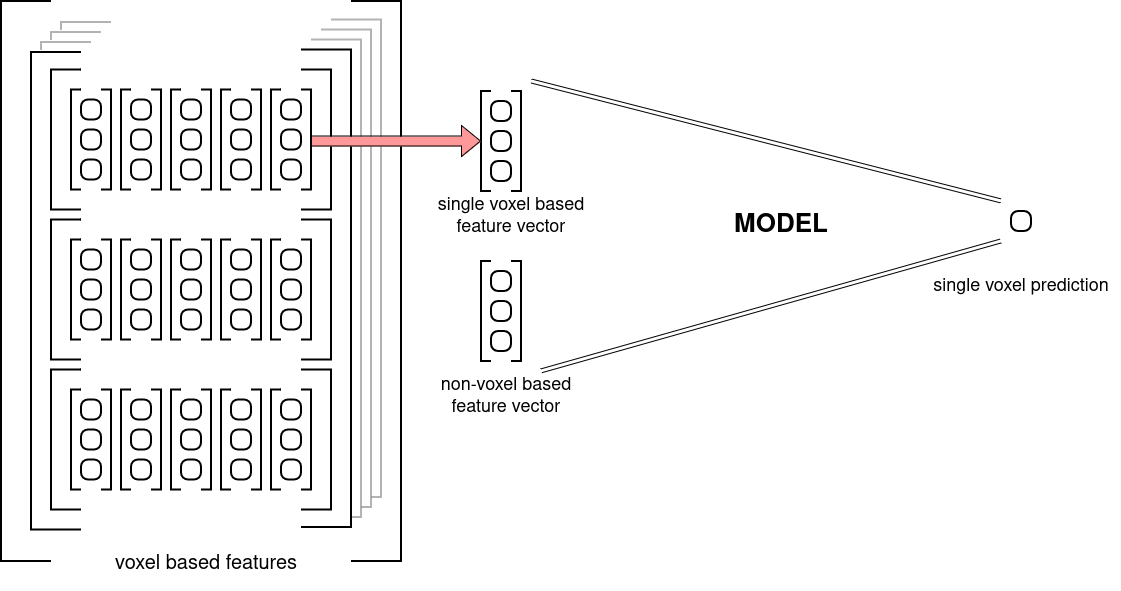
\includegraphics[width=1\textwidth]{model0}
\caption{Simple Model Overview}
\label{fig:model0}
\end{figure}

\textbf{This report will reference to the control/patient spatial data as '{\color{red} Record}'} \emph{("voxel based features" in \reflink{fig:model0}{Figure})} \textbf{and will reference to the individual feature vectors as '{\color{red} Datapoint}'} \emph{("single voxel based feature vector" and "non-voxel based feature vector" in \reflink{fig:model0}{Figure})}\textbf{.} This logical differentiation is needed, as the model only operates on Datapoints and has no global context available, while some preprocessing and evaluation logic should happen on a Record level.

\section{Preprocessing}
\label{sec:preproc}

\subsection{Raw Data}
All provided records are in the \ac{NIfTI} format, first these are need to be understood and parsed. This format stores the raw output of the \ac{MRI} record, and additionally an affine transformation matrix used for aligning different spaces.

\subsubsection{Available Data}
The following records will be preprocessed and read, even if not all of them are going to be used later on it helps providing the largest possible flexibility.

\begin{table}[H]
\centering
\begin{tabular}{|l|l|c|c|l|l|}
\hline
\textbf{Data} & \textbf{Shape} & \textbf{Range} & \textbf{Type} & \textbf{Space} & \textbf{Reference} \\ \hline
\ac{DTI} & (118, 118, 60, 74) & $[0,4096]$ & uint & diffusion & diffusion \\ \hline
Diffusion \ac{FA} & (118, 118, 60) & $[0,~2]$ & float & diffusion & diffusion\_fa \\ \hline
Diffusion \ac{MD} & (118, 118, 60) & $[0,~0.01]$ & float & diffusion & diffusion\_md \\ \hline
Diffusion \ac{RD} & (118, 118, 60) & $[0,~0.01]$ & float & diffusion & diffusion\_rd \\ \hline
T1 & (208, 256, 256) & $[0,~1000]$ & float & t1 & t1 \\ \hline
T1/T2 & (208, 256, 256) & $[0,1]$ & float & d\_aligned & t1t2 \\ \hline
Cortical Targets & (118, 118, 60, 14) & $\{0,1\}$ & bool & diffusion & targets \\ \hline
Relative Connectivity & (118, 118, 60, 14) & $[0,1]$ & float & diffusion & connectivity \\ \hline
Streamline Image & (118, 118, 60, 14) & $[0,5000]$ & uint & diffusion & streamline \\ \hline
\ac{ROI} Mask (Basal Ganglia) & (118, 118, 60, 2) & $\{0,1\}$ & bool & diffusion & mask\_basal \& roi \\ \hline
Brain Mask & (208, 256, 256) & $\{0,1\}$ & bool & t1 & mask\_brain \\ \hline
Basal Ganglia Segmentation & (208, 256, 256) & $[0, 58]$ & uint & t1 & basal\_seg \\ \hline
\end{tabular}
\caption{Raw Data}
\label{tab:datas1}
\end{table}

\subsubsection{Brain Mask}
The provided dataset did not apply the brain masks for the T1 images out of the box so it can be done with a simple element wise multiplication of the T1 image and T1 mask.

\subsubsection{Registration}
The process of aligning different records into the same native space is called "registration". The provided dataset comes with with 2 (3) different spaces, earlier referenced to as t1 and diffusion (and d\_aligned). Most of the data are in diffusion space, thus it is logical to register the rest into the same space. After manual inspection, only 15 records required registration. Out of which 3 only required a tiny translation, and the rest 12 needed a complete affine registration.\par

The image T1/T2 is the odd one out, as it is inherently in a different space from diffusion (due to them being different resolution). But they are aligned into diffusion space. Although they do not need to be registered, this has to be taken into account later on.

\subsubsection{Normalization}
The process of warping each brain into a common space is called "normalization". Applying the \ac{FNIRT} warp fields are more or less straight forward, as two warp fields are provided, one for the diffusion space and one for the T1 space. Note that this process inherently contains the benefits of registration, as it is warping the different images into a common brain shape and space. This also paves the direction of future experiments, as it opens the door to working in either native and normalized space.\par

The only encountered obstacle was with the T1/T2 image. As it is aligned in diffusion space, but \ac{FNIRT} convention ignores the affine transformation of the \ac{NIfTI} format, thus making it's registration useless as the raw data of the t1t2 has nothing to do with the raw diffusion data (due to them being different resolution). The solution is to apply an affine matrix to t1t2's raw data which transforms it into t1's raw data space, after which the t1's \ac{FNIRT} warp field can be applied to the t1t2 image. This affine transformation matrix can be easily calculated from the already given matrices. Let $A$ denote T1/T2's affine matrix and $B$ denote T1's affine matrix (after registration), thus the matrix which transforms the T1/T2 into T1 space is $M = A \cdot B^{-1}$.

\subsubsection{Basal Ganglia Segmentation}

As the tractography of the brain is performed on the diffusion image, it inherently means that the connectivity maps and the roi are in diffusion space. But the basal ganglia's subcortical segmentation is in T1 space. This means that even if they are registered in the same space, they will not have a pixel perfect union due to the different resolutions.

\begin{figure}[H]
\centering
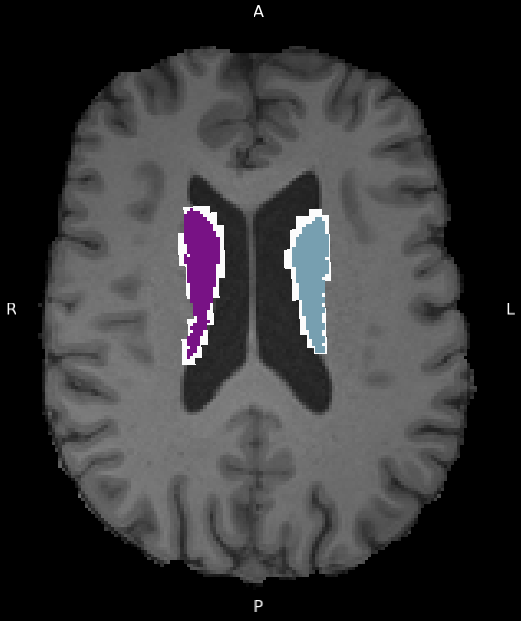
\includegraphics[width=0.3\textwidth]{basal_seg}
\caption{Basal Ganglia Subcortical Segmentation}
\label{fig:basal_seg}
\end{figure}

The figure above visualizes the alignment of the Caudate subcortical region, where the white (larger) region is the Basal Ganglia mask from the diffusion space and the colored (smaller) regions are the Basal Ganglia segmentation from T1 space.\par

In order to keep the data consistent, mapping the segmentation to the Basal Ganglia mask can be done by assigning the same label for each voxel in the basal ganglia as the label of the closest voxel in the subcortical segmentation.

\subsubsection{N-Dim Array}
The used \ac{NIfTI} format stores the raw voxel space and the affine transformation matrix separately, in order to not loose data in the process of interpolating voxels when applying the transformation. But in order to consistently compare voxel data across different spaces (even if they are registered in the same space), the transformation needs to be applied, computing the interpolated voxels in the common space, bringing them into the same raw format of matching X, Y and Z dimensions, and discarding the stored affine matrices.\par

By default the native anatomical space's origin is near the center of mass of the brain, between the ears. This makes sense for medical professionals, when working with \ac{MRI} records, but datastructure wise an array is indexed from 0. Meaning after applying the transformation to the voxel space, the yielded array will only contain one quadrant of the record as the rest are clipped in the negative regions. Thus the space is also needed to be translated with the negative vector of the transformed space's bounding box's lower end.\par

The translation value can be calculated by calculating the boundaries of the transformed space's bounding box. Get all 8 corners of the voxel space and apply the transformation matrix to all of them. Then get the min-max coordinates along X, Y and Z from the 8 transformed vectors, yielding the lower and upper bounds of the transformed space's bounding box.\par

It is very important to use the same translation value across different spaces to properly align them in the native space. For example let $D$ and $T$ denote a diffusion and t1 records and $M_D$ and $M_T$ denote their respective transformation matrices. Let $T_D$ and $T_T$ denote their respective translation values. In order to properly align them we need to apply $A_D = (M_D \cdot {\color{red}T_D})$ matrix and $A_T = (M_T \cdot {\color{red}T_D})$ matrix to $D$ and $T$ respectively, with matching ${\color{red}T_D}$ translation values.\par

The last issue is the missaligned shape of the dimensions of the T1 and diffusion records. This can be simply fixed by truncating the excess along each dimension.

\subsubsection{Uniform Shape}
After aligning the data into the same space per record, it is still very likely that the individual records do not have a uniform shape. This is due to them being in native space, some records will contain a smaller volume brain, some will contain a larger, they will not be the same.\par
Due to the per-voxel based prediction model architecture this is not a problem, but fixing this for being able to use the data in a spatial model like a \ac{FCNN} can be simply solved by adding padding to the records in order to match their shapes.
\begin{table}[H]
\centering
\begin{tabular}{|l|l|c|c|}
\hline
\textbf{Data} & \textbf{Volumes} & \textbf{Range} & \textbf{Type} \\ \hline
diffusion & 74 & $[0,4096]$ & float16 \\ \hline
diffusion\_fa & 1 & $[0,2]$ & float16 \\ \hline
diffusion\_md & 1 & $[0,0.01]$ & float16 \\ \hline
diffusion\_rd & 1 & $[0,0.01]$ & float16 \\ \hline
t1 & 1 & $[0,1000]$ & float16 \\ \hline
t1t1 & 1 & $[0,1]$ & float16 \\ \hline
targets & 14 & $\{0,1\}$ & bool \\ \hline
connectivity & 14 & $[0,1]$ & float16 \\ \hline
streamline & 14 & $[0,5000]$ & float16 \\ \hline
mask\_basal & 2 & $\{0,1\}$ & bool \\ \hline
mask\_brain & 1 & $\{0,1\}$ & bool \\ \hline
basal\_seg & 6 & $\{0,1\}$ & bool \\ \hline
\end{tabular}
\caption{Uniform Data}
\label{tab:datas2}
\end{table}

\subsection{Quality Control}

Having a low count of records means that if there are even just a few outliers, it can heavily affect the end result. Thus all data were manually inspected to make sure they are as clean as possible.

\subsubsection{Mismatched Data}

Looking through the diffusion, diffusion\_fa, diffusion\_md and diffusion\_rd images, 2 records' \ac{FA}, \ac{MD} and \ac{RD} images were seemingly from completely different patients. Thus the \ac{FA}, \ac{MD} and \ac{RD} images were omitted for 2 records.

\subsubsection{Garbled Data}

Looking through the subcortical segmentation of the Basal Ganglia revealed that 1 record had a garbled segmentation. Thus, said basal\_seg image was omitted for 1 record.\par
And one record had a garbled T1 \ac{FNIRT} warp field. Said record was entirely omitted from the normalized set of records.

\subsubsection{Missing Data}

Looking through the relative connectivity and streamline images, 3 records were missing these images, said 3 records were completely omitted, as these records are effectively missing the labels.\par
And the t1t2 images were missing for 10 records, but these were not omitted completely as the t1 images were present for these records, thus experiments only concerning the t1 can have a bit more available data.

\subsection{Radiomics Features}

\citelink{radio}{Although the term is not strictly defined, radiomics generally aims to extract quantitative, and ideally reproducible, information from diagnostic images, including complex patterns that are difficult to recognize or quantify by the human eye.} Using these features is key, as there are not nearly enough data for \ac{NN} based features extraction such as a \ac{CNN}.\par

Extracting the voxel based radiomic features has two main parameters to tune, the bin width and the kernel width. Where the binning parameter(s) influence how the intensity values of the image are binned, and the kernel size influences the size of the 'sliding window' similar to a convolution.\par

The two approaches for binning are absolute discretization and relative discretization. Where in the prior one, a fixed bin width is chosen and in the latter one, a fixed number of bins are chosen and the bin width scales relatively according to the min-max voxel values. \citelink{bin}{This study found that "The absolute discretization consistently provided statistically significantly more reproducible features than the relative discretization."} Relying on this information, the obvious choice to start with is the absolute discretization.\par
The bin width and the kernel width will be tuned in later experiments. And possibly features calculated with different settings will be concatenated and used simultaneously for better results. The used default values will be 25 and 5 for the bin and kernel widths respectively.\par
The following types of radiomic features will be used:
\begin{table}[H]
\centering
\begin{tabular}{|l|c|}
\hline
\textbf{Feature Type} & \textbf{Number of Features} \\ \hline
first order & 18 \\ \hline
\ac{GLCM} & 23 \\ \hline
\ac{GLSZM} & 16 \\ \hline
\ac{GLRLM} & 16 \\ \hline
\ac{NGTDM} & 5 \\ \hline
\ac{GLDM} & 14 \\ \hline
3D shape & 17 \\ \hline
\end{tabular}
\caption{Radiomic Feature Types}
\label{tab:radf0}
\end{table}

\subsubsection{Voxel Based}
The 92 features in \reflink{tab:radf1}{Table} will be calculated voxel based. Shape features do not makes sense to calculate voxel based as it would just describe the shape of the used kernel, which is constant and independent from the input image.

\subsubsection{Non-Voxel Based}

However, the additional shape features in \reflink{tab:radf2}{Table} do make sense for the non-voxel based features. As it can be computed for each target region, both hemispheres of the \ac{ROI} and the entire brain.

\subsection{Coordinates}

One additional input that can be included in the experiments is the coordinates. Although this approach only makes sense in normalized space, where the images from different records are aligned. This theoretically would allow the model to learn certain anatomical markers based on the location of the voxel, adding a type of global context to the input of the model.\par
Furthermore, this approach can be adopted to the native space, by constructing the normalized coordinate map and then 'de-normalizing' them with an inverse \ac{FNIRT} warp field.

\subsection{Data Augmentation}

The only data augmentation that makes sense involves applying small rotation values to the input images in their native space before calculating radiomic features. Applying transformations to the already extracted features is illogical, as interpolating between voxels in feature space is unlikely to yield the same results as computing features after transforming the input images. In summary, any spatial data transformations should be performed upstream. Furthermore, data augmentation only makes sense in native space, as by definition such transformations would make the normalized image pointless.

\subsection{Scaling and Normalization}
\label{sec:norm}

As the extracted features have very different ranges, it makes sense to follow the standard practice of scaling the data to a fixed range. Inspecting the histogram of some of the radiomic features reveals that most of them follow a bell curve with moderate standard deviation, such as \reflink{fig:hist_fie}{Figure} (Firstorder Energy).\par

\begin{figure}[H]
\centering
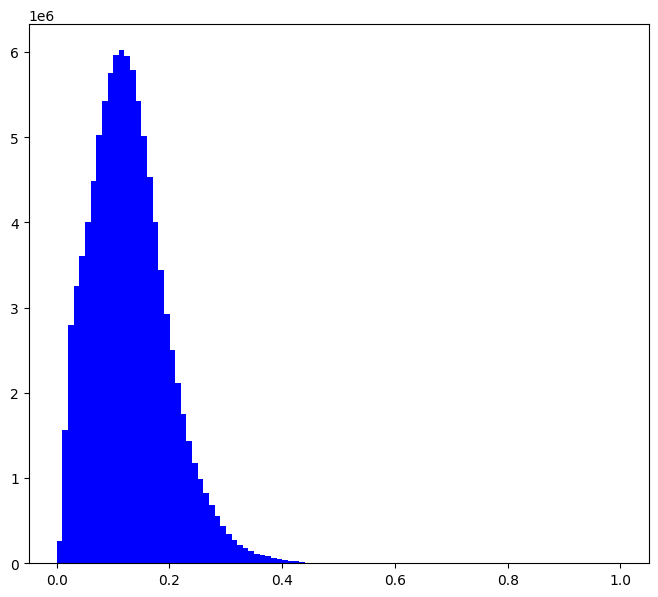
\includegraphics[width=0.4\textwidth]{hist_firstorder_energy}
\caption{Histogram: Firstorder Energy}
\label{fig:hist_fie}
\end{figure}

However, some other features like \reflink{fig:hist_gls}{Figure} (GLDM Small Dependence High Gray Level Emphasis) and \reflink{fig:hist_ngb}{Figure} (NGTDM Busyness) have a very skewed distribution, the latter one being the most extreme case. This skewing can be mitigated by applying logarithm to the offending features.

\begin{figure}[H]
\centering
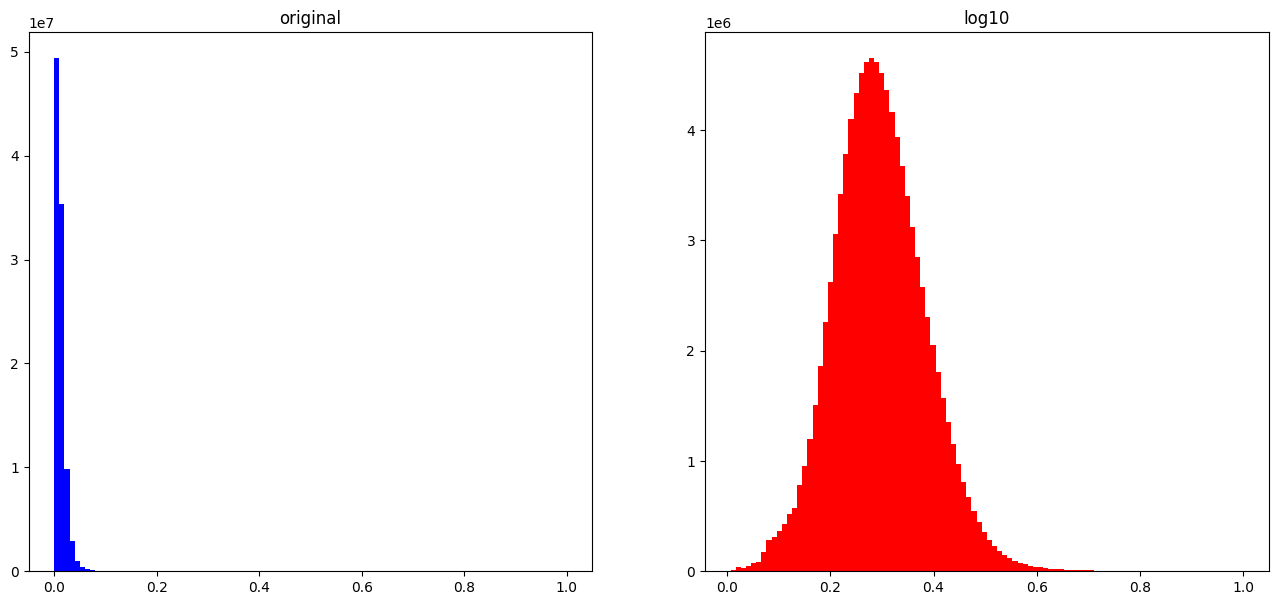
\includegraphics[width=0.8\textwidth]{hist_gldm_small}
\caption{Histogram: GLDM Small Dependence High Gray Level Emphasis}
\label{fig:hist_gls}
\end{figure}

\begin{figure}[H]
\centering
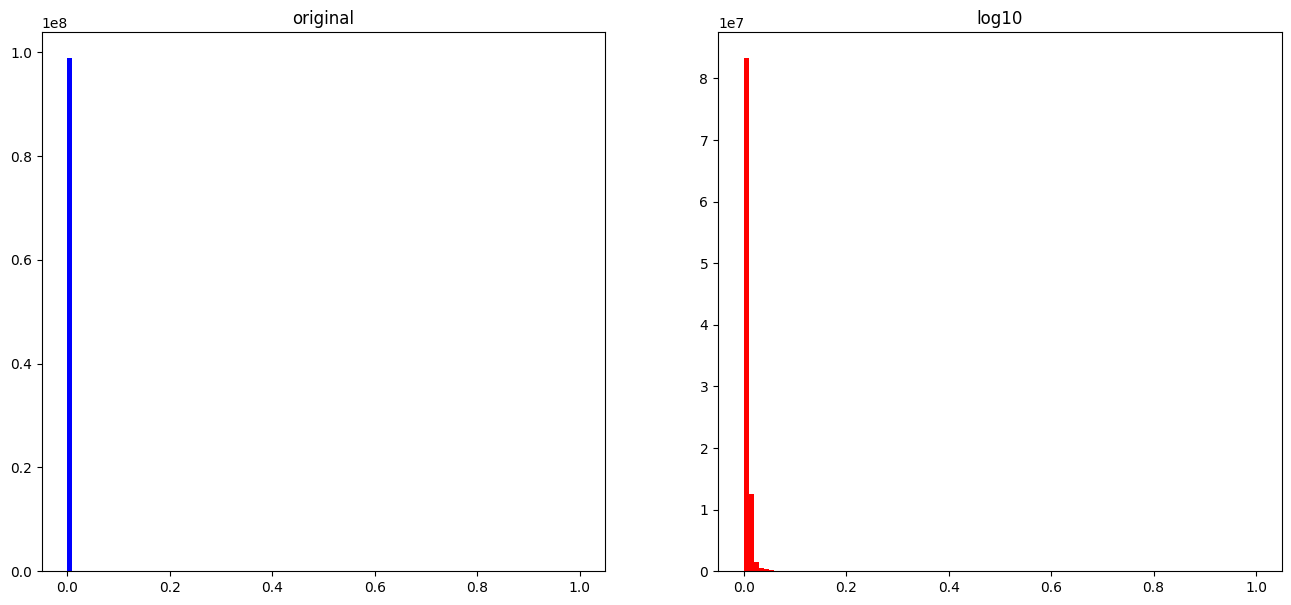
\includegraphics[width=0.8\textwidth]{hist_ngtdm_busyness}
\caption{Histogram: NGTDM Busyness}
\label{fig:hist_ngb}
\end{figure}

Besides the standard benefits of making the optimization process more stable and efficient, and reducing the sensitivity to outliers. It also have some less evident benefits.\par
Although it is very subtle, but storing these records in float16 inherently looses some information. This loss is not a problem for the features that have a healthy distribution, but in the more extreme cases it can cause compression artifacts visible even to the naked eye, such as the very subtle loss of detail in \reflink{fig:gls}{Figure}. And in the most extreme case it can even render the entire feature useless like in \reflink{fig:ngb}{Figure}. While the normalized features have no problem storing this fine detail in float16.\par
This makes the system much more robust from a practical perspective; as depending on the hardware, some GPUs are much more efficient at computing in float16. And it also halves the memory and storage requirements, as in float32 a sinlge MRI image of 92 volumes (for the 92 features) takes up around 1GB of space.\par
Selecting which features need normalization is done programmatically, and the exact selection criteria is detailed in \reflink{app:imp-norm}{Appendix}.

\subsection{Data Balancing}

Working with highly unbalanced data can be challenging, and balancing it does not necessarily going to help the model's generalization capability. Thus, a method for partially balancing the data will be used, where the bins of the unbalanced data will be up-sampled by a ratio of the difference of the number of datapoints in the bin (compared to the bin with the maximum number of datapoints). \reflink{fig:bal_sub}{Figure} demonstrates how a ratio 1 means perfectly balanced data, 0 means unbalanced data. And how the ratios in between are approximately preserving the shape of the distribution and partially balance the data.

\begin{figure}[H]
\centering
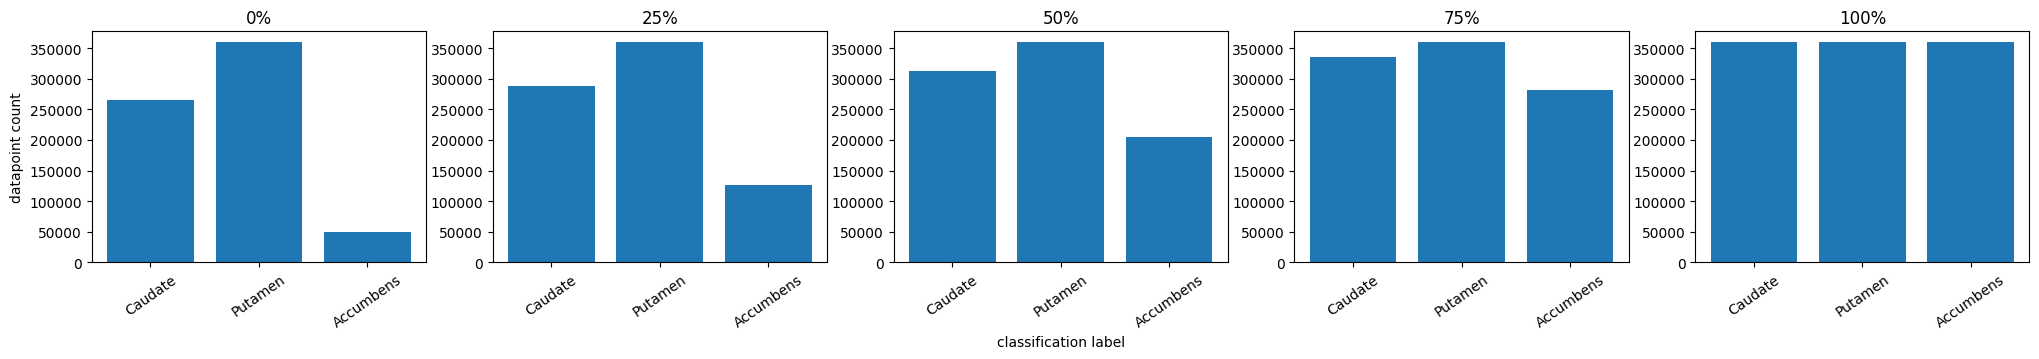
\includegraphics[width=1\textwidth]{bal_subcortical}
\caption{Balance: Subcortical}
\label{fig:bal_sub}
\end{figure}

For the diffusion\_md and diffusion\_fa, which are regression problems and have continuous labels, binning can be used to create artificial groups which can be balanced.

\begin{figure}[H]
\centering
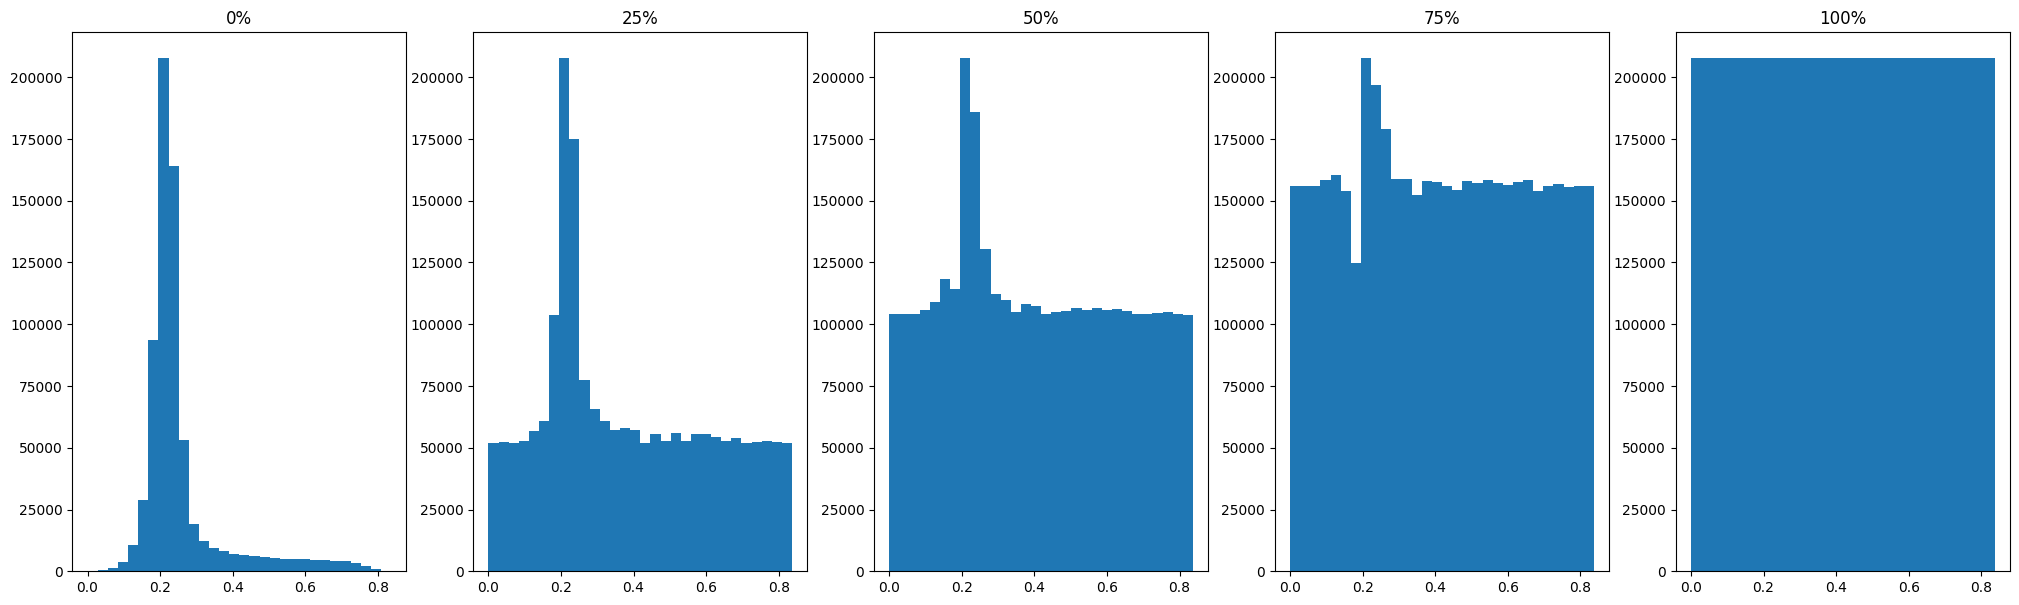
\includegraphics[width=1\textwidth]{bal_diffusionmd}
\caption{Balance: Diffusion MD}
\end{figure}

\begin{figure}[H]
\centering
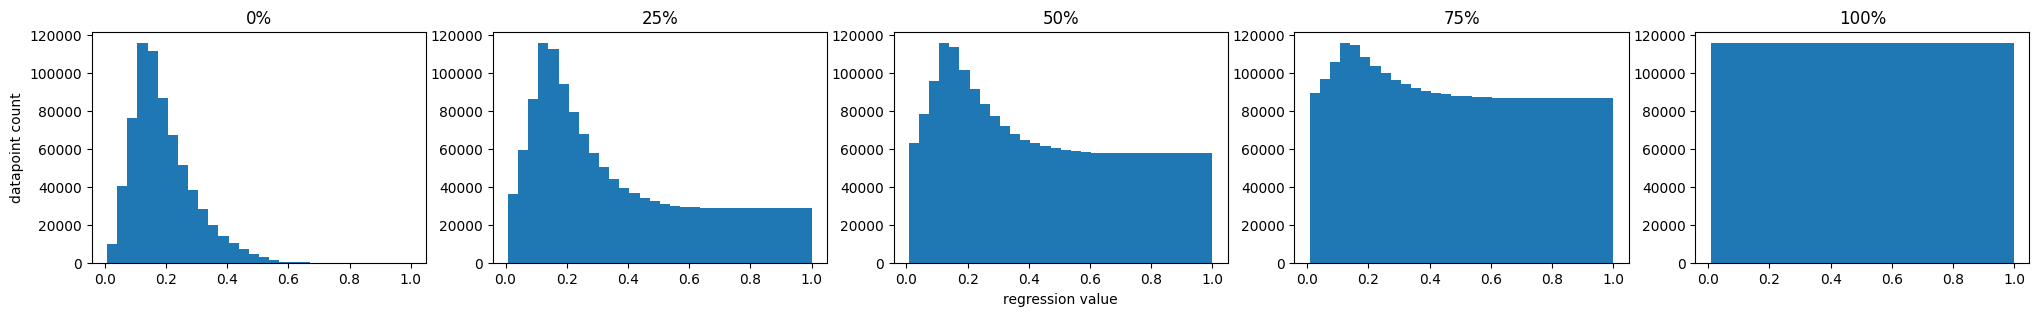
\includegraphics[width=1\textwidth]{bal_diffusionfa}
\caption{Balance: Diffusion FA}
\end{figure}

\begin{figure}[H]
\centering
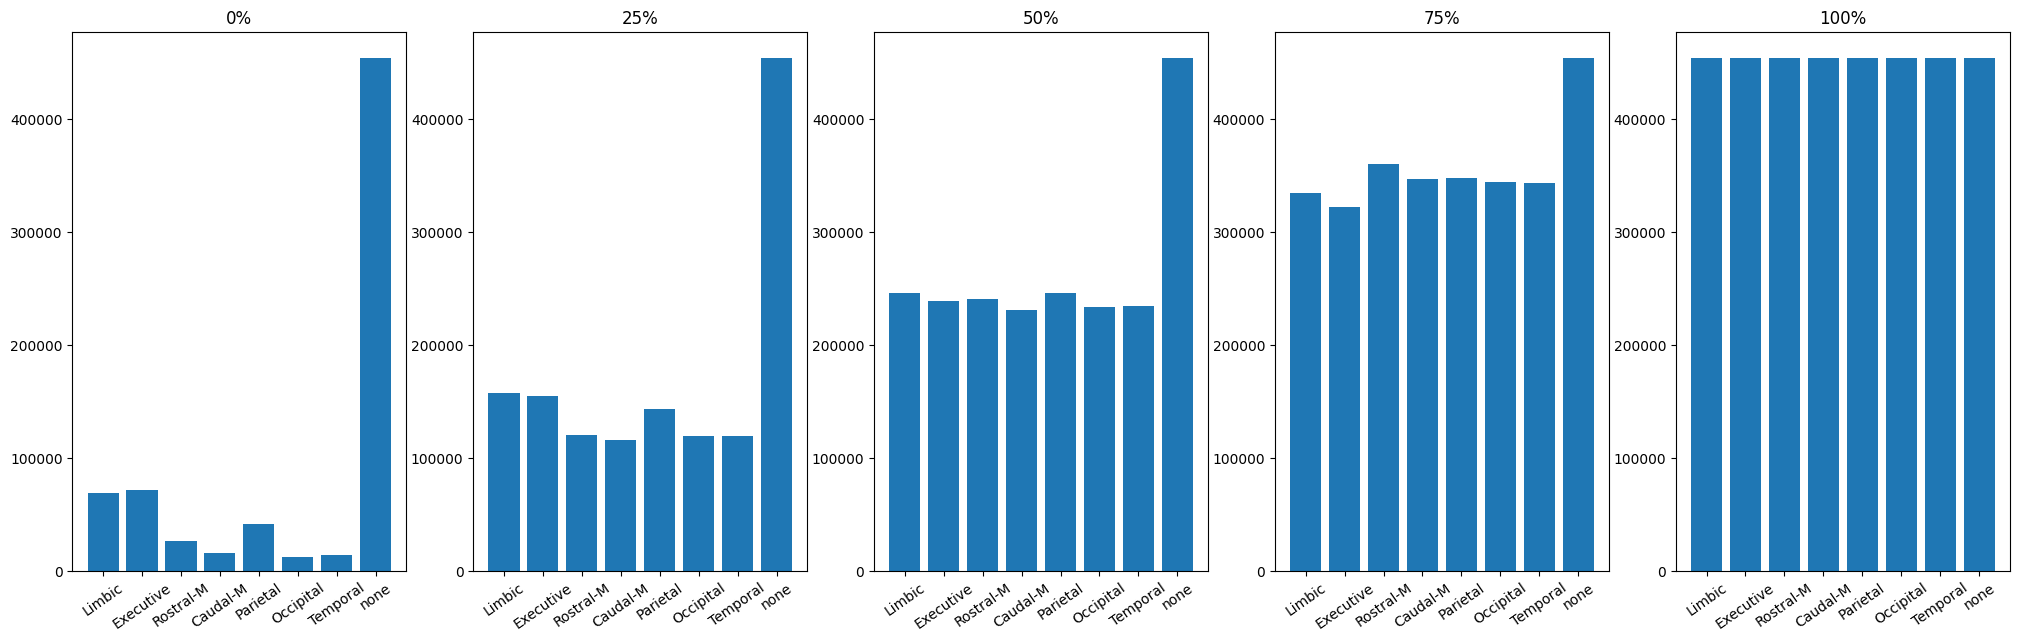
\includegraphics[width=1\textwidth]{bal_connectivity}
\caption{Balance: Relative Connectivity (thresholded at $0.6$ \& binarized)}
\end{figure}

\subsection{Clinical Data}
\label{sec:clinical}

There are additional clinical data available for the Patient records. \citelink{cap}{Disease severity can be characterized in terms of \ac{CAP} score. Providing a measure of cumulative exposure to the mutant HTT gene.} This widely accepted and used \ac{CAP} score is available for all patients.\par
Another, newer metric for characterizing disease severity is the \citelink{cUHDRS}{\ac{cUHDRS}}. This is calculated from 4 other basic metrics: Total Functional Capacity, Total Motor Score, Symbol Digit Modalities Test and Stroop Word Reading. These are available for most patients, with a handful exceptions.\par
And there are a total of 91 available clinical features, with relatively a lot of missing data on some of these features. There are 8 additional patients available in the clinical data. These can be used to aid the data imputation for the missing values, and can be omitted afterwards, as these have no corresponding \ac{MRI} records.\par
All clinical features were scaled the range of 0-1 with min-max scaling (per feature). And euclidean distance was used for the following imputation process. The imputation strategy itself consisted of 2 steps, first the few missing \ac{cUHDRS} values were imputed from the \ac{CAP} score. And then the remaining features were imputed from the combined \ac{CAP} and \ac{cUHDRS} values.

\subsection{Relative Connectivity}
\label{sec:conpre}

Relative Connectivity describes the ratio of the number of streamlines going into each cortical target. This means that the Streamline record can be converted into Relative Connectivity by simply dividing by the total number of streamlines in each voxel. With the additional inbetween step of filtering some noise, by thresholding the streamlines at 250 (5\% of the total 5000 streamlines), meaning any voxel which has less than 250 streamlines to a target region are set to zero.\par
Then the relative connectivity could be converted into a label, by picking the label of the cortical target to the highest connection per voxel. However this would yield very noisy labels, as these ratios can be quite balanced between the multiple cortical targets, for example voxels with ratios of 0.31/0.29/0.3/0.1. To mitigate this, the relative connectivity can be thresholded at a value higher than 0.5, meaning a label can only be picked for a voxel if at least half of the connections are going to a single target.\par
But this also means that there can be voxels without labels. This can be dealt with introducing an artificial 'Not Connected' label for these voxels.\par
To achieve the best results and filtering, 0.6 was chosen for the thresholding value, as it also filters potential 50-50 situations and only allows labeling strong connections.

\section{Evaluation}

\subsection{Train, Validation and Test Splits}
\label{sec:travaltes}

There are 2 important aspects when splitting the data into Train/Validation/Test groups. In order to truly validate the model's generalization capability, the split must happen on a record level and not on a datapoint level. This means that our model can only learn on certain records, and it can be validated on records that it never seen before, not even partially. This has the consequence of that the split will not follow the defined ratio on a datapoint level, as it could happen that by pure chance the train split contains records with larger volumes, resulting in having a bit more datapoints than the validation split.
\begin{figure}[H]
\centering
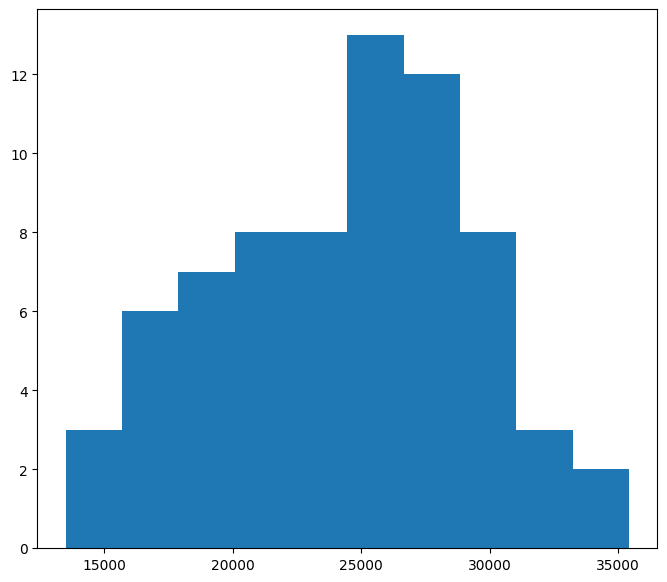
\includegraphics[width=0.5\textwidth]{split}
\caption{Distribution of Records in relation to Datapoints}
\label{fig:hist_split}
\end{figure}
In practice the lower end of datapoint count per record is around half of the higher end. \reflink{fig:hist_split}{Figure} shows the distribution of both Control and Patient records and both Left and Right datapoints. During experimentation, with $0.8$ Train split and $0.5$ Validation/Test split, the datapoint ratios stayed in the range of $0.8\pm0.02$ and $0.5\pm0.06$ for the two split ratios.\par
Furthermore to avoid introducing bias in the case of experiments with mixed Control and Patient records, the ratio of Controls/Patients must be constant across the different splits. This is required as Controls and Patients can have vast differences due to neurodegeneration. An extra caveat is having another ratio that must also be kept constant for the same reason, which is the symptomatic and asymptomatic patients, as they can also have vast differences due to different stages of neurodegeneration.

\subsection{Accuracy and Pearson Correlation}
\label{sec:eval}

There will be 3 groups of metrics for evaluating each model. First is the 'raw' (will also be referenced as 'train') metric group, which is computed on the datapoints that were extracted with the same hyperparameters as the datapoints during the training process. Meaning that this metric group best reflects how the model performs on the different splits, such as if the model was trained with a balancing of $0.5$, all splits will be balanced the same way and the metrics will be computed on a datapoint level (the same way as how it is naturally computed in the loss function).\par
The second and third groups are for comparing model performances in between models and are for practical evaluation. The difference is that the metrics in this case are computed for each record, and then averaged out inbetween records. This means that it is computed on a record level instead of a datapoint level, resulting in the elimination of potential bias coming from the deviation from the number of datapoints per records. It also means that these metric groups will inherently ignore data balancing, as it operates on a record level.\par
And the 2nd metric group is computed in native space, while the 3rd is computed in normalized space. This means that if the model operates in native space, the normalized metrics will be computed by predicting the datapoints for each record, then the spaital record is reconstucted from the datapoints and warped to normalized space, and then the datapoints are extracted from the normalized spaital prediction, and compared against the normalized labels (This process would be computationally quite expensive, so the implementation does not follows this exact logic, but numerically it is doing the same; more information on this in \reflink{app:imp-pre}{Appendix}). This way the models can have comparable metrics even if they operate in different spaces.












\chapter{Experiments}
\label{experiments}

The hyperparameters listed in \reflink{tab:hypcom}{Table} were kept constant during all of the experiments:
\begin{table}[H]
\centering
\begin{tabular}{|l|c|}
\hline
\textbf{Hyperparameter} & \textbf{Value} \\ \hline
Train Split & 0.8 \\ \hline
Validation/Test Split & 0.5 \\ \hline
Model Type & \ac{FNN} \\ \hline
Optimizer & Adam \\ \hline
\end{tabular}
\caption{Hyperparameters: Common}
\label{tab:hypcom}
\end{table}

\section{Subcortical Segmentation}

Before addressing the primary objectives of predicting \ac{FA}, \ac{MD}, and Relative Connectivity, a precursor experiment was conducted, focusing on segmenting the Basal Ganglia into its subcortical regions: Caudate, Putamen, and Accumbens. This experiment served as a sanity check to validate the feasibility of the overall project. It was intentionally crafted to be simple.\par
Given the simplicity of the problem, extensive tuning was unnecessary, as it worked very well almost from the start. The set of hyperparameters reported in \reflink{tab:subhyp}{Table} remained constant during these experiments:
\begin{table}[H]
\centering
\begin{tabular}{|l|c|}
\hline
\textbf{Hyperparameter} & \textbf{Value} \\ \hline
Control/Huntington Records & Control Only \\ \hline
Left/Right Hemisphere Datapoints & Both \\ \hline
Space & Native \\ \hline
Image & T1 \\ \hline
Scaling/Normalization & Normalized Voxel Based Features \\ \hline
Hidden Layers & 1024 \rightarrow 512 \rightarrow 256 \rightarrow 128 \\ \hline
Loss & Categorical Crossentropy \\ \hline
Activation & Sigmoid (softmax for the output layer) \\ \hline
Learning Rate & 0.001 \\ \hline
Batch Size & 10000 \\ \hline
Early Stopping Patience & 7 \\ \hline
\end{tabular}
\caption{Hyperparameters: Subcortical}
\label{tab:subhyp}
\end{table}
The reasoning behind the initial choices of these parameters is straightforward. The T1 image and native space were chosen, because those are the simplest to acquire in practice. Thus, if the model performs well with those, there is no need for more complicated inputs. Including both hemispheres would hopefully result in a model which can generalize better. Only using control datapoints should translate into less variance between the general characteristics of the datapoints, as it does not contain patients with neurodegeneration. The number and sizes of the hidden layers were choosen based on the potential size of the input layer, which should range from $92$ (single set of voxel based features) up to $\sim1000-2000$ including many different kernel sizes and non-voxel based features as well. The choice of the categorical crossentropy loss function and the output layer's softmax activation function are standard practices for a classification problem. The Sigmoid activation function should work fine without having to deal with exploding gradients and dieing relu problems. The default learning rate of the Adam optimizer in TensorFlow is chosen, while a batch size of $10,000$ seems appropriate for a train split size of $1,000,000$ datapoints. The early stopping patience of 7 epochs should also be good enough to prevent overfitting and stop the training in time, but it will be evaluated on the basis of the learning curves and the accuracy of the model.\par
The metric used for evaluating model performance on the Train/Validation/Test splits is Accuracy. The 'k' and 'b' notations stand for kernel and bin, where k5 means a kernel width of 5mm, b25 means an absolute bin size of 25, and b10r means relative binning with 10 bins. In the case of multiple kernel sizes denoted by a dash, it naturally only means odd kernel sizes. \reflink{tab:expsub}{Table} reports the results of the subcortical experiments:

\begin{longtable}[H]{|r|p{9cm}|l|l|l|r|}
\hline
 & \textbf{Experiment} & \textbf{Train} & \textbf{Val} & \textbf{Test} & \textbf{Input Layer} \\ \hline
1. & \textbf{Voxel Features k5\_b25} & $68.9$ & $69.1$ & $72.4$ & $92$  \\ \hline
2. & \emph{Voxel Features k5\_b25} \newline \textbf{Non-Voxel Features of Target Regions b25} & $73.2$ & $68.9$ & $72.5$ & $1576$ \\ \hline
3. & \emph{Voxel Features k5\_b25} \newline \textbf{Non-Voxel Features of ROI b25} & $75$ & $74.3$ & $78.5$ & $304$ \\ \hline
4. & \emph{Voxel Features k5\_b25 \newline Non-Voxel Features of ROI b25} \newline \textbf{Non-Voxel Features of Brain b25} & $74.5$ & $70.4$ & $70.3$ & $410$ \\ \hline
5. & \emph{Voxel Features k5\_b25} \newline \textbf{Non-Voxel Features of ROI b10 b25 b50 b75} & $71.2$ & $70.6$ & $74.3$ & $856$ \\ \hline
6. & \textbf{Voxel Features k5\_b25 - k21\_b25} \newline \emph{Non-Voxel Features of ROI b25} & $94.5$ & $94.1$ & $95.1$ & $1040$ \\ \hline
7. & \textbf{Voxel Features k5\_b25 - k21\_b25} & $95$ & $94.6$ & $93.7$ & $828$ \\ \hline
8. & \emph{Voxel Features k5\_b25 - k21\_b25 \newline Non-Voxel Features of ROI b25} \newline \textbf{Balance Ratio 0.5} & $94.9$ & $94.4$ & $94.9$ & $1040$ \\ \hline
9. & \emph{Voxel Features k5\_b25 - k21\_b25 \newline Non-Voxel Features of ROI b25} \newline \textbf{Balance Ratio 1} & $95.9$ & $95.5$ & $95.9$ & $1040$ \\ \hline
\caption{Hyperparameter Tuning: Subcortical}
\label{tab:expsub}
\end{longtable}

The best performing model was that of experiment 9, which achieved a near $96\%$ accuracy with practically no overfitting. The biggest improvement during the experiments was to include many different kernel sizes for the voxel based features. The additional non-voxel based features of the \ac{ROI} yielded only a small improvement, while balancing the data yielded a marginal improvement, by reducing overfitting.\par
Examples of the true/predicted records can be found in \reflink{fig:pred-tra-sub}{Figures} \reflink{fig:pred-tes-sub}{-}. And the loss training curves can be found in \reflink{fig:curve-sub}{Figure}.

\section{Methodology}

The experimentation from this point on, will be divided into 4 main groups:
\begin{itemize}
  \item Native - T1
  \item Native - T1/T2
  \item Normalized - T1
  \item Normalized - T1/T2
\end{itemize}

These groupings enable a comprehensive investigation aligned with the state-of-the-art approaches discussed in Section \ref{sec:stateoftheart}. By examining these four experimental groups, this study aims to systematically evaluate the feasibility of synthesizing \ac{DTI} related images. This approach provides a thorough basis for understanding the impact of imaging modalities and spatial normalization on the proposed methodology's performance.

\subsection{Native or Normalized Space}

The use of native and normalized spaces is essential for addressing certain variances inherent in the dataset. Working in normalized space helps reduce participant specific differences and minimizes the effects of neurodegeneration related changes, such as volumetric variations in the basal ganglia.\par
Normalization also mitigates minor misalignments between \ac{DTI} and anatomical \ac{MRI} records that might occur in native space, despite optimal affine registration. Such discrepancies can arise due to independent data acquisition processes, physiological movements, or independent preprocessing steps.\par
Nevertheless, the impact of these factors on model performance is not straightforward. The complex interplay between these sources of variance and their influence on the outcome necessitates experimentation to determine whether native or normalized space offers a performance advantage or whether the choice has no significant effect.

\subsection{T1 or T1/T2 Imaging}

The inclusion of T1 imaging is justified by its widespread historical availability and integration into many clinical protocols. On the other hand, the exploration of T1/T2 imaging stems from recent studies highlighting its correlation with myelin content. These studies suggest that the T1/T2 ratio may serve as a 'bridge' between anatomical \ac{MRI} and \ac{DTI} data, potentially enabling a more reliable extraction of structural connectivity information.

\subsection{Further Hyperparameters}

The same set of core experiments will be run for all 4 groups, and some additional experiments will be run per group, depending on how they perform. The experiments will consider the following aspects:
\begin{itemize}
  \item Single/Many Different Kernel Sizes for Voxel Based Features
  \item Additional Non-Voxel Based Features
  \begin{itemize}
    \item Single/Many Different Bin Sizes
  \end{itemize}
  \item Control/Patient/Both Records
  \item Left/Right/Both Hemisphere Datapoints
  \item Additional Clinical Features for Patient Records
  \item Additional Coordinate Map Features
  \item Scaled Voxel Based Features (not normalized)
  \item Different Bin Sizes for Voxel Based Features
  \item Different Balance Ratios
  \item Data Augmentation in Native Space
\end{itemize}

These aspects facilitate a comprehensive exploration of standard data science principles, enabling the optimization of structural connectivity image synthesis. Additionally, the approach incorporates robustness assessments by experimenting with different configurations, such as splitting or combining Control/Patient records, and Left/Right hemisphere data points. Moreover, it incorporates experimental factors such as additional clinical data for patients, which may help address the increased variance within these records.

\subsection{Missing Records}

In order to be completely fair when comparing model performances, only records which are available for all 4 groups of experiments should be used. In practice, the records reported in \reflink{tab:misrec}{Table} were missing:
\begin{table}[H]
\centering
\begin{tabular}{|l|c|}
\hline
\textbf{Record} & \textbf{Missing Amount} \\ \hline
Normalized & 1 \\ \hline
T1/T2 & 10 \\ \hline
Diffusion \ac{FA} \& \ac{MD} & 2 \\ \hline
\end{tabular}
\caption{Missing Records}
\label{tab:misrec}
\end{table}
This meant that for the Diffusion \ac{FA} \& \ac{MD} experiments there were a total of 13 records omitted, yielding 57 records in total, out of which 29 are Control and 28 are Patient records. And for the Relative Connectivity experiment, 11 records were omitted, yielding 59 records in total, out of which 30 are Control and 29 are Patient records.\par
As additional experiments for the groups with more available data (such as T1, where 10 more records could be included), these records can be appended to the train split on the best performing model, which could increase the model's generalization capability and performance.

\subsection{Architecture Tuning}

For the best performing model, the architecture will be further tuned, considering the following aspects:
\begin{itemize}
  \item Number of Layers and Layer Sizes
  \item Activation Function
  \item Batch Size
  \item Learning Rate
  \item Dropout Normalization
  \item Early Stopping Patience
\end{itemize}

\section{Diffusion Fractional Anisotropy Regression}

All the results of the \ac{FA} experiments can be found in \reflink{fig:fa-nat-t1}{Tables} \reflink{fig:fa-arch}{-}.
The baseline starting experiment tried to predict the \ac{FA} from a single set of voxel based radiomic features, with a kernel size of 5 and with the same starting hyperparameters (\reflink{tab:subhyp}{Table}) that were also used in the subcortical segmentation (with exception of the used loss function, which is Mean Squared Error instead of the Categorical Crossentropy).\par
The next few experiments were trying to determine how does each set (target regions, \ac{ROI}, and entire brain) of non-voxel based features affect the model performance. The observations were more or less consistent between the 4 different groups of experiments (Native-Normalized \& T1-T1/T2), with the final consensus being that the inclusion of the entire brain's non-voxel based features are yielding the best results, with an improvement of 5-10\% in correlation compared to the baseline. Including many different bin sized non-voxel based features worsened the model performance by 0-3\%.\par
The biggest improvement occurred with the inclusion of many different kernel sized voxel-based features, with an improvement of 10-15\%. And, surprisingly, after removing the non-voxel based features, T1 experiments performance further improved by 1-2\%, while worsening the T1/T2 experiments by 0-1\%.\par
The experiments consistently showed the model performing much better on the Control records (by 5-10\%), as compared to the Patient records, with much less overfitting and better correlation.\par
The inclusion of the clinical features behaved inconsistently between the 4 groups of experiments. For the native T1, the inclusion of the \ac{CAP} and \ac{cUHDRS} features marginally improved the model performance, and for the normalized T1/T2 it improved model performance by 4-5\%, while for the native T1/T2 and normalized T1, it worsened the model performance by 5-10\%. The overall Patient records even with the best performing clinical features, were still performing worse than the Control records.\par
As expected, mixing Control and Patient records did perform worse than Control records only, but only with 1-5\% correlation.\par
The inclusion of coordinates, did not affect the T1 models' performance, but it did marginally increase the T1/T2 models' performance.\par
The use of only min-max scaling, and not normalizing the datapoints, resulted in marginally worse performance.\par
Increasing the bin size for the voxel based radiomic features marginally decreased the model performance.\par
Balancing the data was a bit inconsistent between the groups of experiments, but the balance ratio of 1 usually resulted in a marginally worse, and a balance ratio of 0.5 resulted in a marginally better performance.\par
Adding the 10 extra T1 records to the training split for the T1 experiment only resulted in a marginal improvement for the native space, and a 2\% improvement for the normalized space.\par
After combining all of the best configurations, the best performing model was the T1 normalized model, with Control records only, and with added T1 records, without any additional non-voxel based features. It reached a final correlation of \textbf{84.4/84.6/82.8} for the train/val/test splits in native space, and \textbf{84.6/84.9/82.9} in normalized space.\par
Tuning the model architecture by searching different layer sizes and numbers, activation functions, dropout normalization, adjusting learning rate and batch size, only increased the model’s overfitting, without any actual benefits.\par
Examples of the true/predicted records can be found in \reflink{fig:pred-tra-fa}{Figures} \reflink{fig:pred-tes-fa}{-}. And the loss training curves can be found in \reflink{fig:curve-fa}{Figure}.

\begin{figure}[H]
\centering
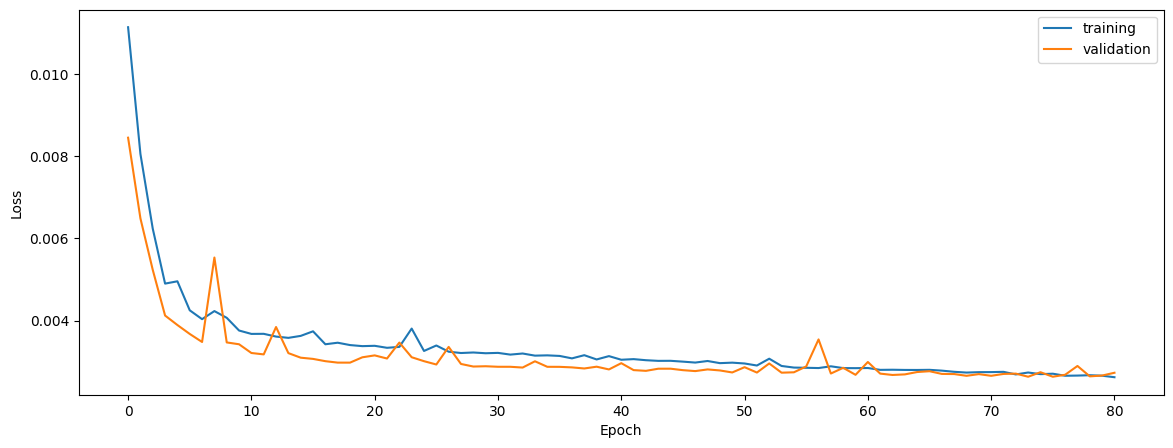
\includegraphics[width=0.7\textwidth]{fa_curve}
\caption{Training Curve: Diffusion Fractional Anisotropy}
\label{fig:curve-fa}
\end{figure}

\begin{figure}[H]
\centering
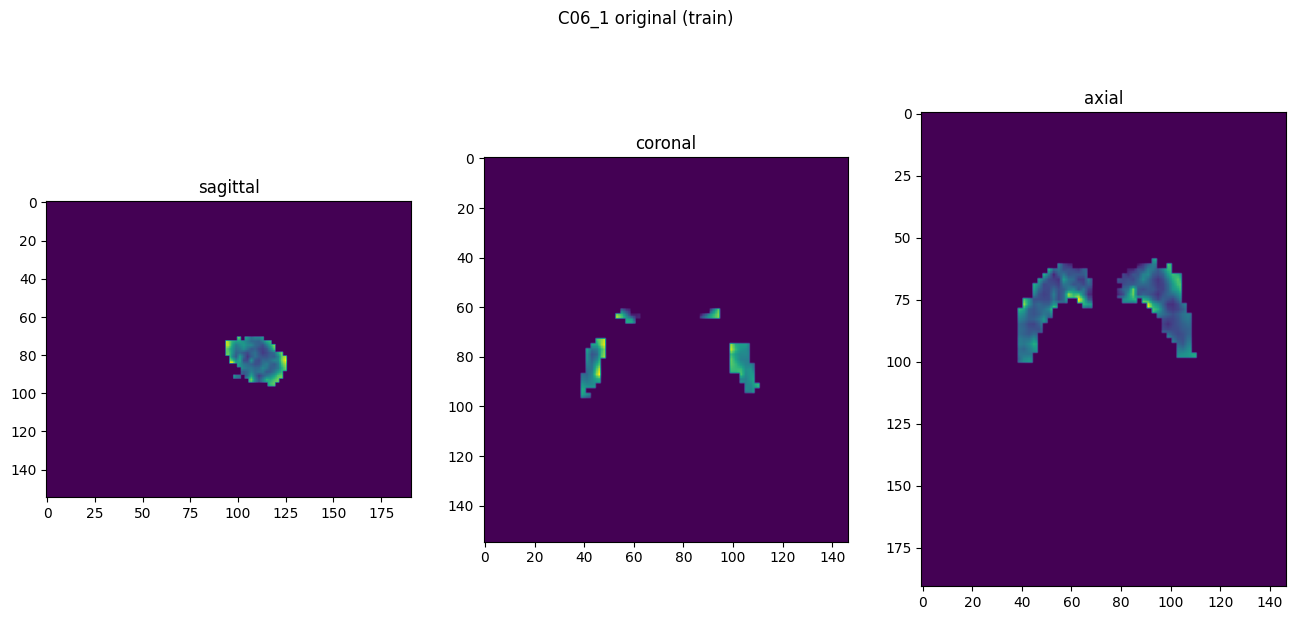
\includegraphics[width=0.65\textwidth]{fa_train_o}
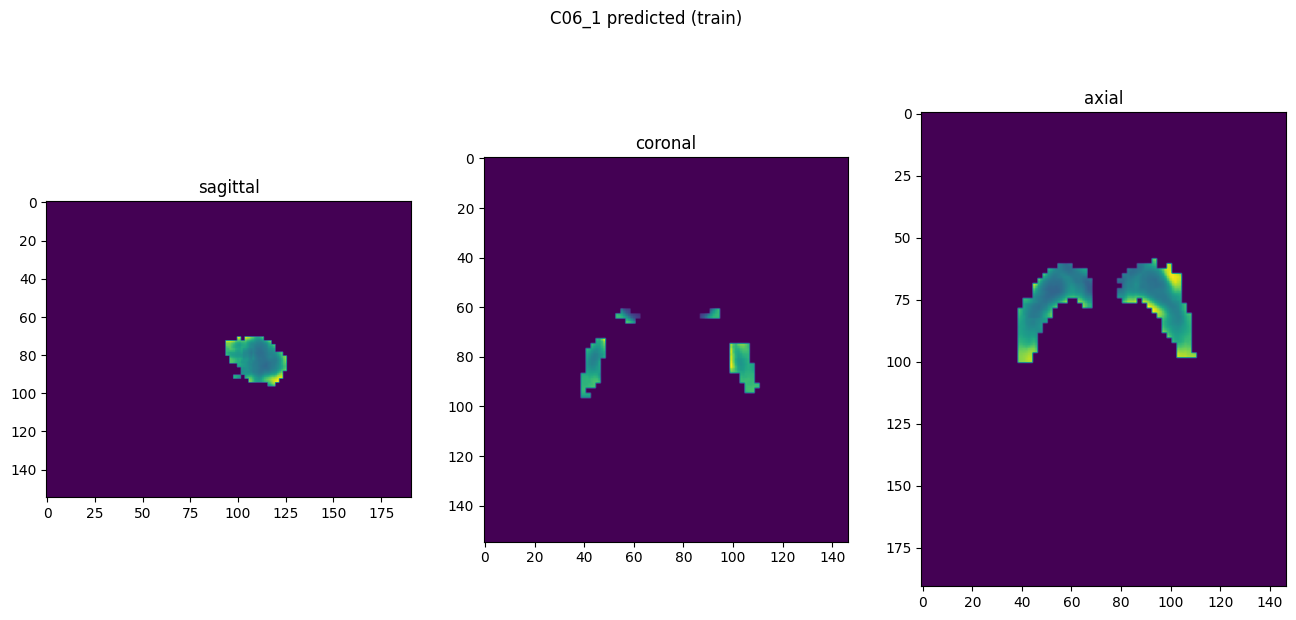
\includegraphics[width=0.65\textwidth]{fa_train_p}
\caption{Train Predictions: Diffusion Fractional Anisotropy}
\label{fig:pred-tra-fa}
\end{figure}

\begin{figure}[H]
\centering
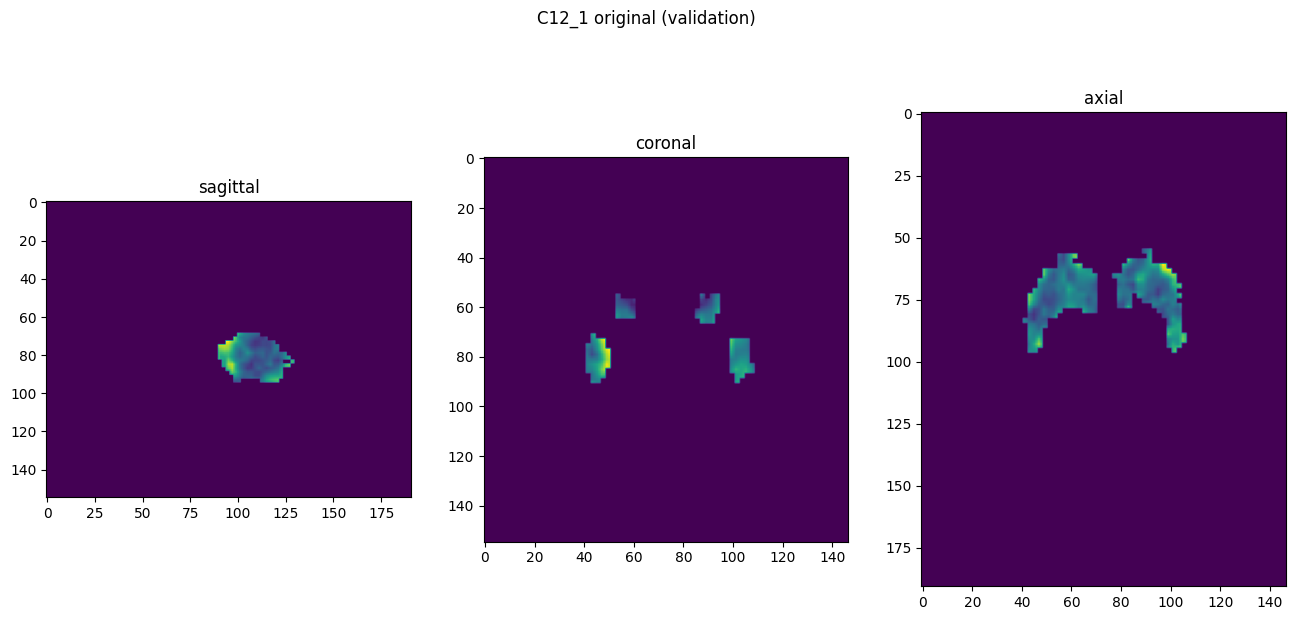
\includegraphics[width=0.65\textwidth]{fa_val_o}
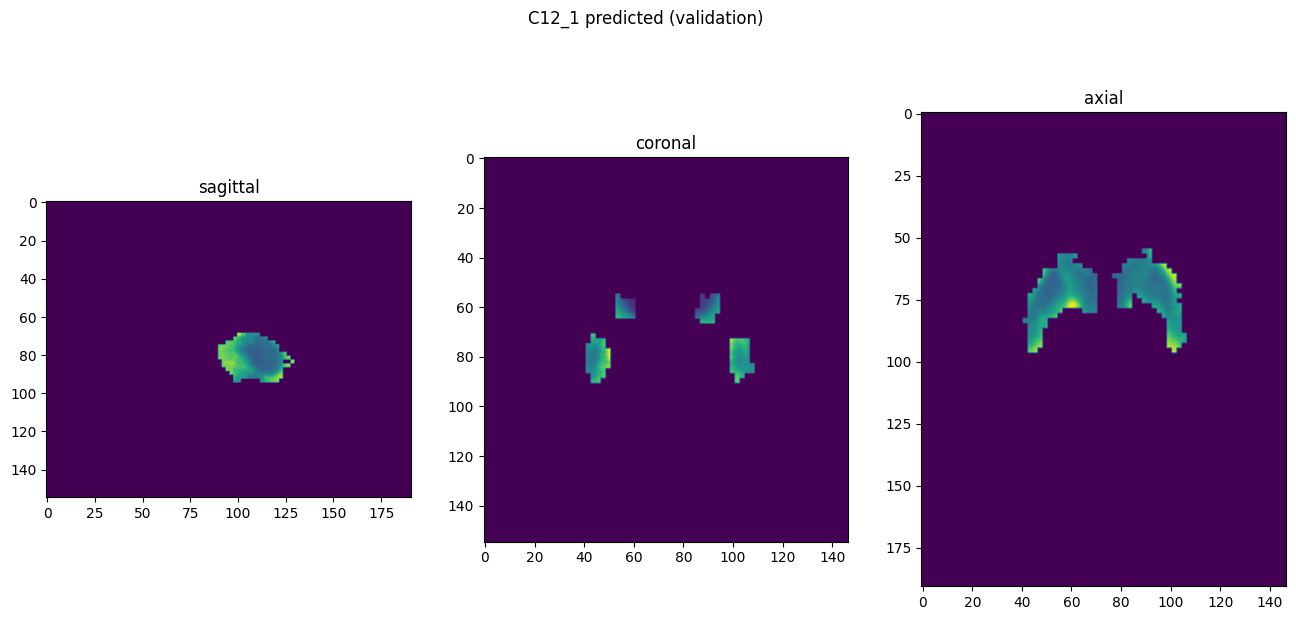
\includegraphics[width=0.65\textwidth]{fa_val_p}
\caption{Validation Predictions: Diffusion Fractional Anisotropy}
\label{fig:pred-val-fa}
\end{figure}

\begin{figure}[H]
\centering
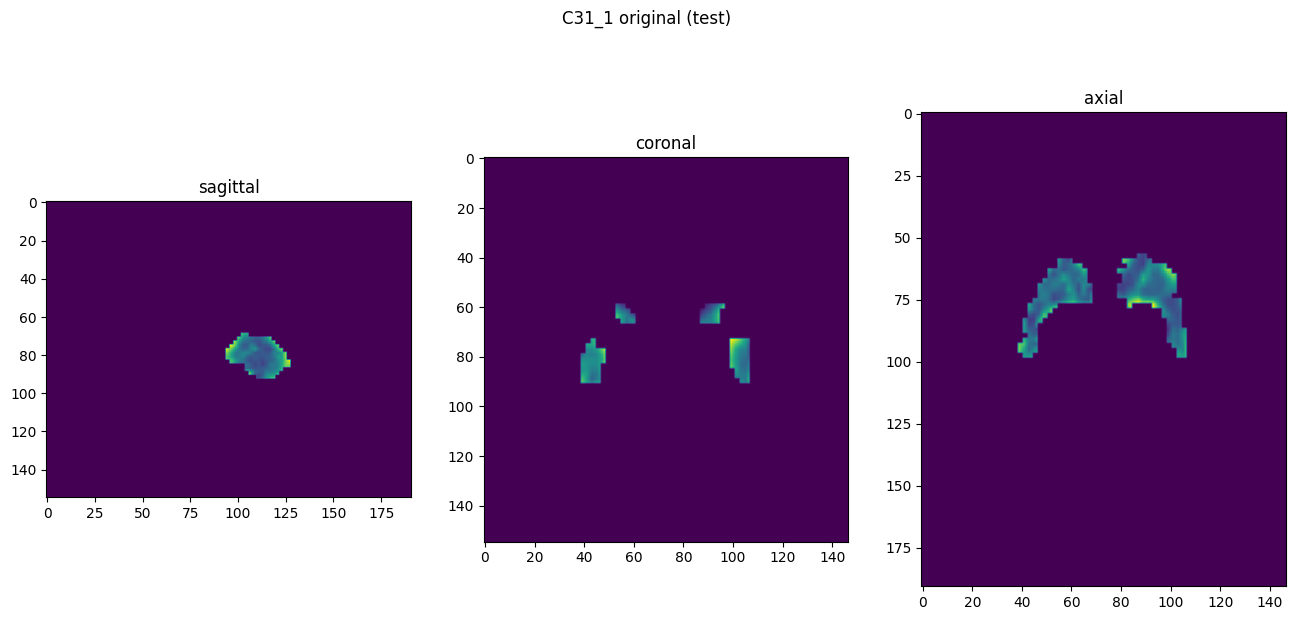
\includegraphics[width=0.65\textwidth]{fa_test_o}
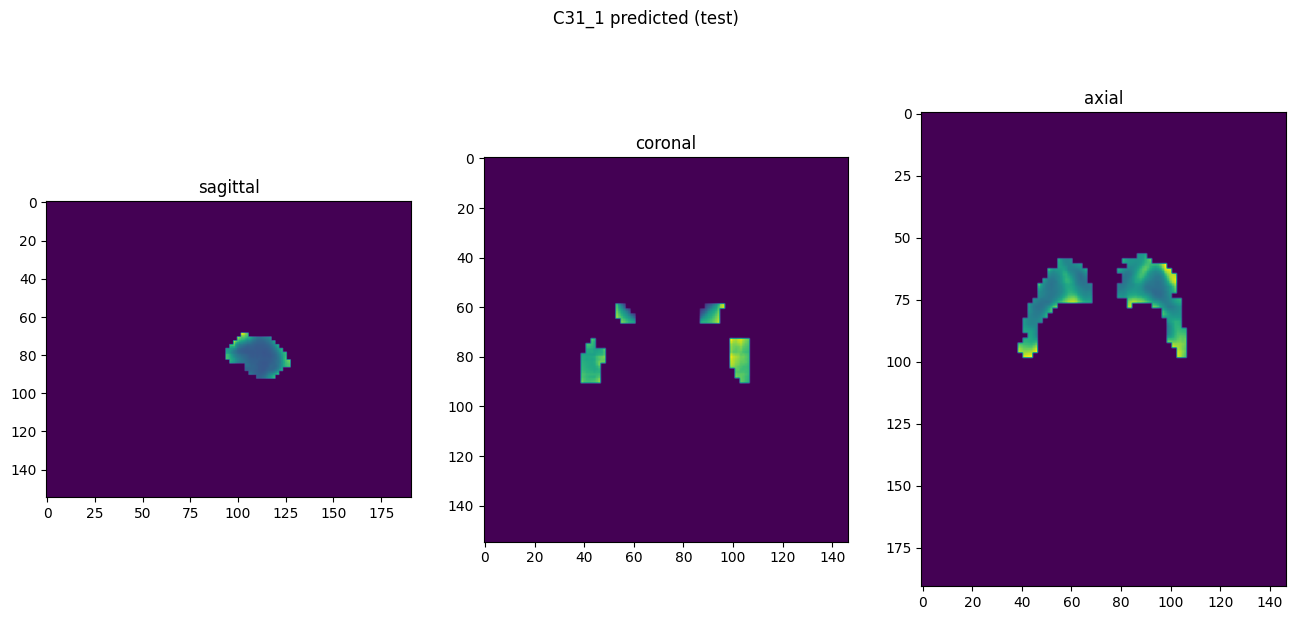
\includegraphics[width=0.65\textwidth]{fa_test_p}
\caption{Test Predictions: Diffusion Fractional Anisotropy}
\label{fig:pred-tes-fa}
\end{figure}

\section{Mean Diffusivity Regression}

A similar set of experiments were run for predicting \ac{MD}. The compilation of results is available from \reflink{fig:md-nat-t1}{Tables} \reflink{fig:md-arch}{-}. These experiments were showing strong performance from the onset: even the baseline Native T1 experiment with a single set of voxel based features resulted in a correlation of 94\% without any overfitting.\par
No significant observation can be made here, besides the Patient records performing marginally worse.\par
The best performing model was Native T1, on the Control records only, with the additional non-voxel based features of the entire brain, and many different voxel based kernel sizes. It reached a final correlation of \textbf{94.7/95.5/95.1} for the train/val/test splits in native space, and \textbf{95.4/95.7/96.3} in normalized space.\par
Tuning the model architecture, by searching different layer sizes and numbers, activation functions, dropout normalization, adjusting learning rate and batch size, did not increase the performance, not even for the train split, indicating that this is the absolute best this model can do.\par
Examples of the true/predicted records can be found in \reflink{fig:pred-tra-md}{Figures} \reflink{fig:pred-tes-md}{-}. And the loss training curves can be found in \reflink{fig:curve-md}{Figure}.

\begin{figure}[H]
\centering
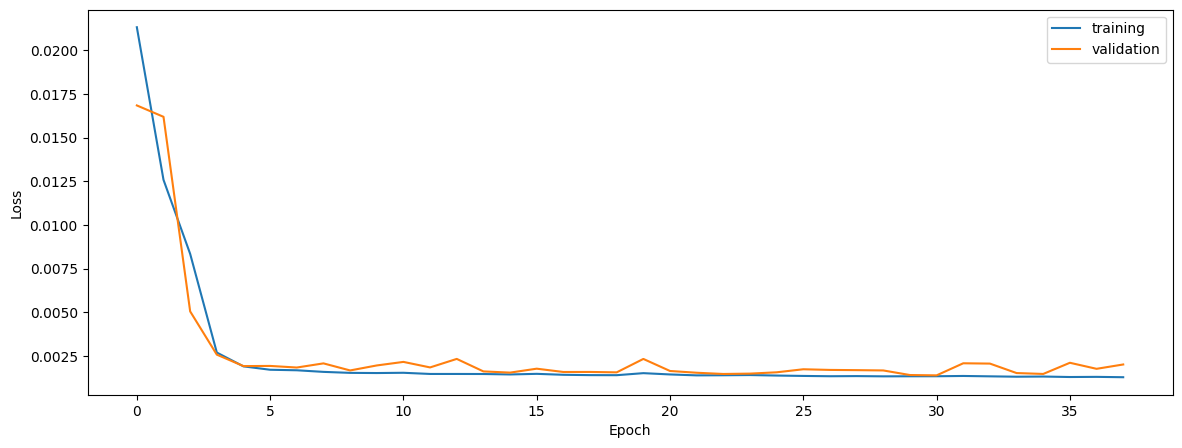
\includegraphics[width=0.7\textwidth]{md_curve}
\caption{Training Curve: Mean Diffusivity}
\label{fig:curve-md}
\end{figure}

\begin{figure}[H]
\centering
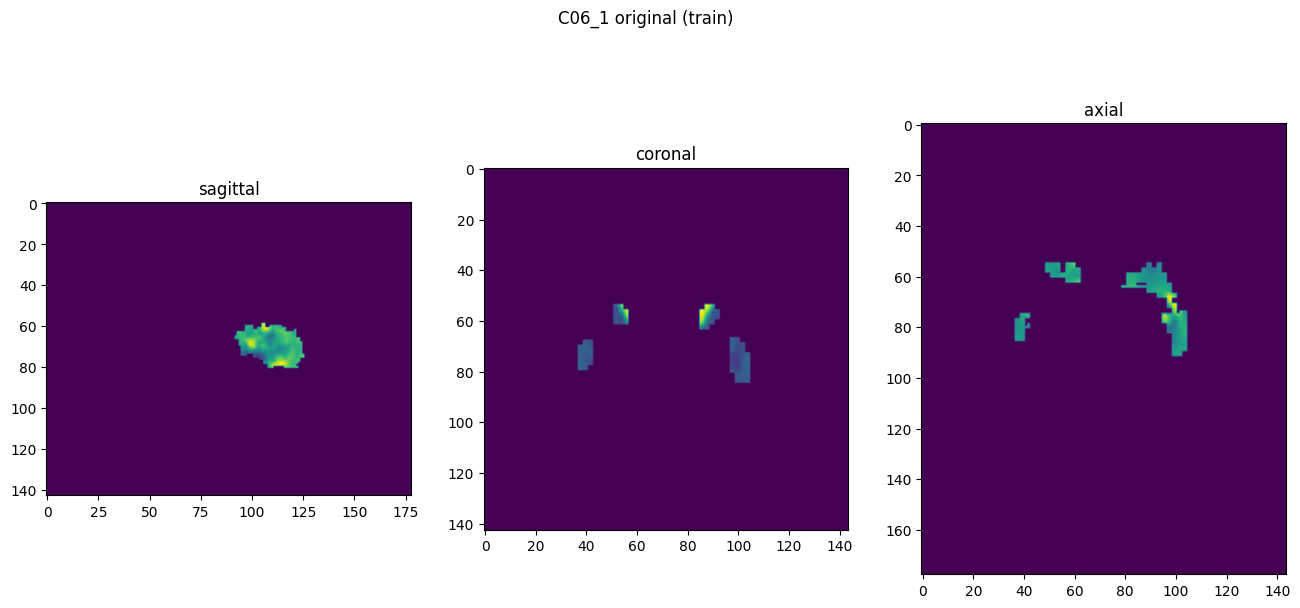
\includegraphics[width=0.65\textwidth]{md_train_o}
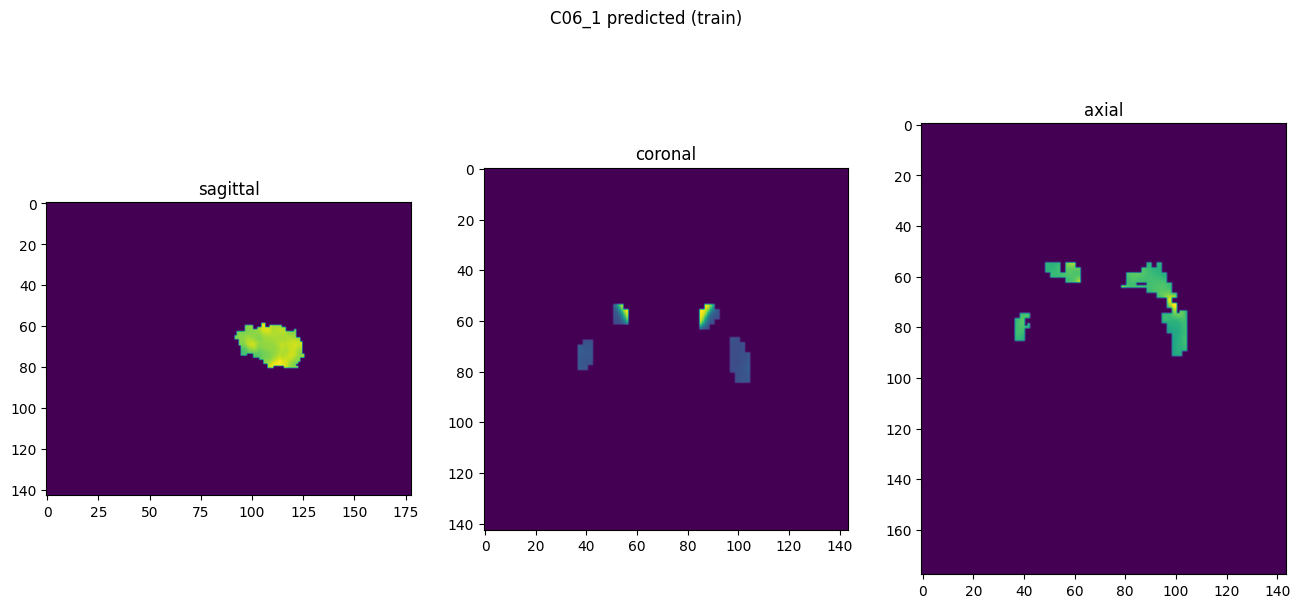
\includegraphics[width=0.65\textwidth]{md_train_p}
\caption{Train Predictions: Mean Diffusivity}
\label{fig:pred-tra-md}
\end{figure}

\begin{figure}[H]
\centering
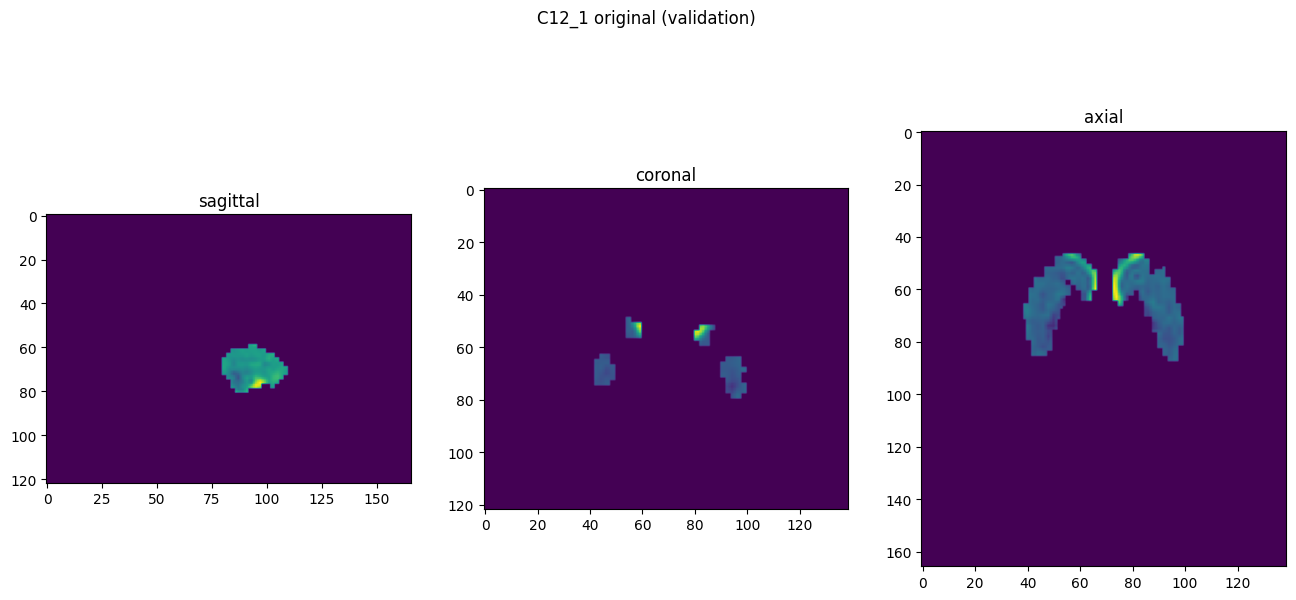
\includegraphics[width=0.65\textwidth]{md_val_o}
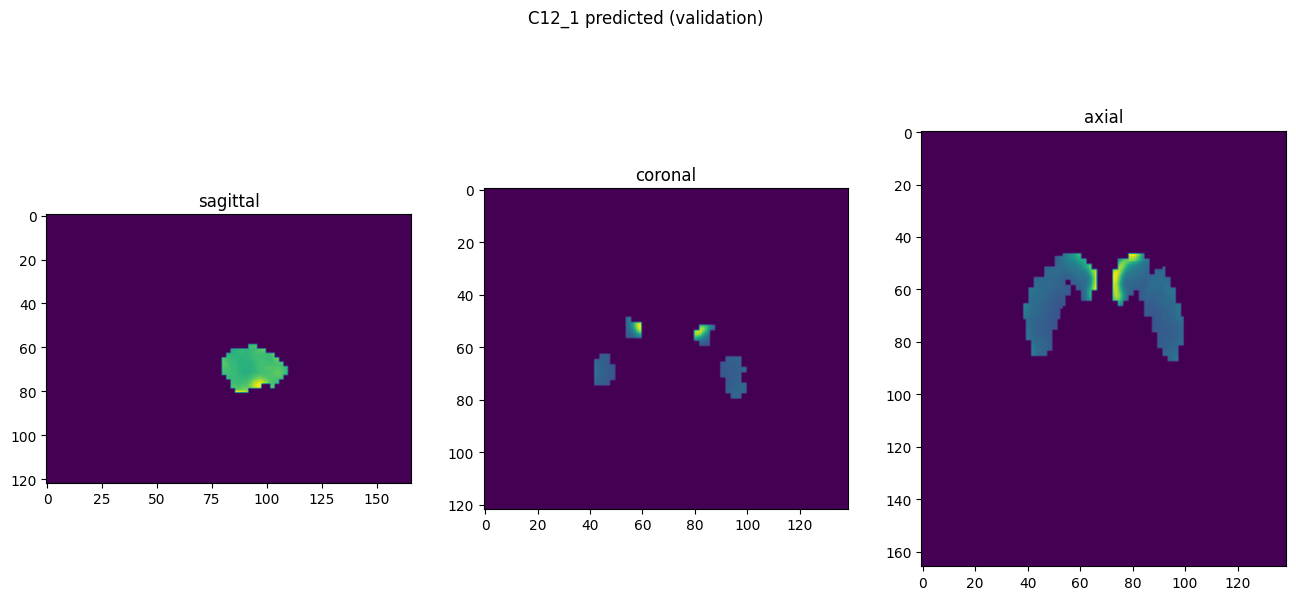
\includegraphics[width=0.65\textwidth]{md_val_p}
\caption{Validation Predictions: Mean Diffusivity}
\label{fig:pred-val-md}
\end{figure}

\begin{figure}[H]
\centering
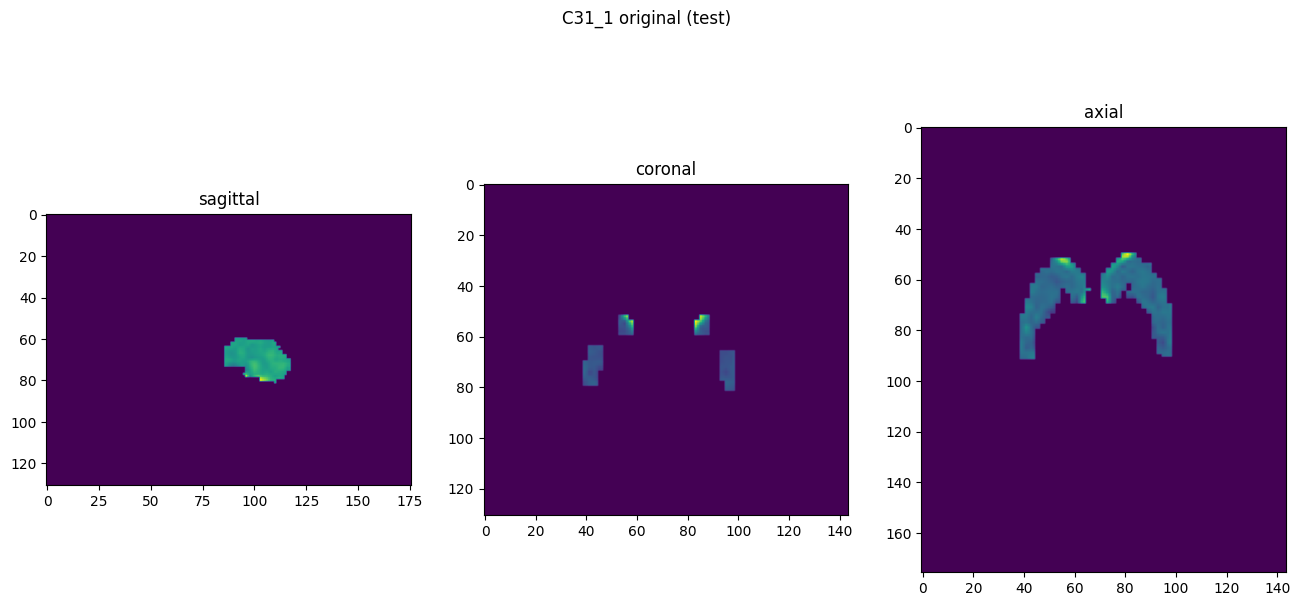
\includegraphics[width=0.65\textwidth]{md_test_o}
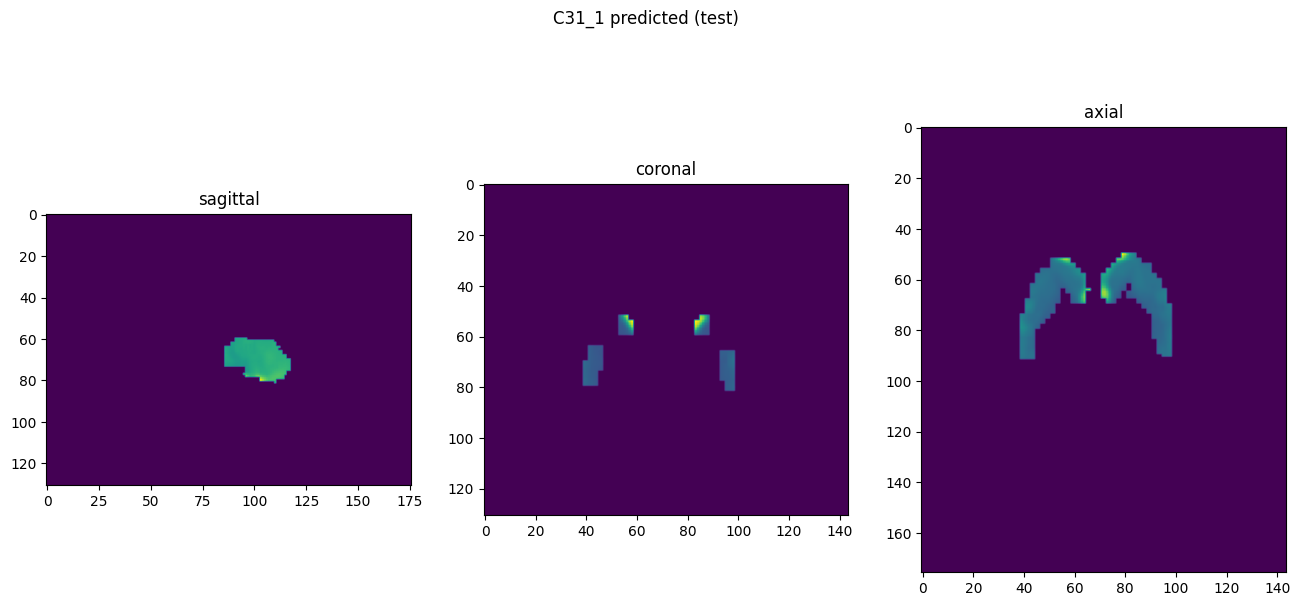
\includegraphics[width=0.65\textwidth]{md_test_p}
\caption{Test Predictions: Mean Diffusivity}
\label{fig:pred-tes-md}
\end{figure}

\section{Relative Connectivity Segmentation}

All numerical results corresponding to the Relative Connectivity Segmentation experiments can be found in \reflink{fig:con-nat-t1}{Tables} \reflink{fig:con-arch}{-}.
The baseline starting experiment is trying to predict the Relative Connectivity (preprocessed with the method described in \reflink{sec:conpre}{subsection}) from a single set of voxel based radiomic features, with a kernel size of 5, and with the same starting hyperparameters (\reflink{tab:subhyp}{Table}) that were also used in the subcortical segmentation.\par
The subsequent experiments aimed to determine how does each set (target regions, \ac{ROI}, and entire brain) of non-voxel based features affect the model performance. The results were fairly consistent between the 4 different group of experiments (Native-Normalized \& T1-T1/T2), with the final consensus being that the inclusion of non-voxel based features does not improve model performance.\par
The biggest improvement (5-10\%) was obtained with the inclusion of many different kernel sized voxel-based features.\par
The experiments consistently showed the model performing much better on the Control records, compared to the Patient records, with much less overfitting and better accuracy (by 2-5\%).\par
The inclusion of the clinical features yielded inconsistent results between the four groups of experiments. For the normalized experiments, it mostly had no effect, or made it marginally worse, while for the native T1 experiments, the inclusion of \ac{CAP} and \ac{cUHDRS} features marginally improved the model performance. Finally, for the native T1/T2, it increased train/validation performance substantially, but yielded worse test performance, due to strong overfitting.\par
Mixing Control and Patient records only performed marginally worse than using only Control records.\par
Including coordinates, consistently increased accuracy by 1-2\%.\par
Only using min-max scaling, and not normalizing the datapoints, resulted in marginally worse performance.\par
Increasing the bin size for the voxel based radiomic features marginally decreased the model performance.\par
Balancing the data consistently and substantially decreased performance (depending on the balance ratio by 5-20\%)\par
The addition of the 10 extra T1 records as part of the training split for the T1 experiments did not affect the model performance.\par
After combining all of the best configurations, the best performing model was the T1 normalized model, with Control records only, with the additional coordinate inputs, without any additional non-voxel based features. It reached a final accuracy of 72.6/72.1/73.3 for the train/val/test splits in native space, and 73.2/71.9/73 in normalized space.\par
After tuning the model architecture, by searching different layer sizes and numbers, activation functions, dropout normalization, adjusting learning rate and batch size, the only thing which marginally increased model performance was lowering the batch size to $10^3$ and lowering the learning rate to $10^{-4}$, yielding a final accuracy of \textbf{73.3/72.9/73.4} in native space, and \textbf{73.5/72.3/73.4} in normalized space.\par
As these numbers can be misleading due to the highly unbalanced data, the best way to get more insight on how the model is performing is by observing the confusion matrices in \reflink{fig:conf_prec}{Figure} and \reflink{fig:conf_rec}{Figure}. Matrices in \reflink{fig:conf_prec}{Figure} are normalized along the predicted label axis, effectively displaying the precision in the diagonals; in \reflink{fig:conf_rec}{Figure}, they are normalized along the true label axis, effectively displaying the recall in the diagonals. The first and most evident observation is that the unbalanced nature of the data is reflected on the confusion matrix, as the over-represented 'not connected' datapoints have a much better precision and recall than the rest.\par
Also, the model is more effective at minimizing false positives than it is at minimizing false negatives, since it generally has a higher precision than recall for practically all labels (except the 'not connected').\par
Examples of the true/predicted records can be found in \reflink{fig:pred-tra-con}{Figures} \reflink{fig:pred-tes-con}{-}. And the loss training curves can be found in \reflink{fig:curve-con}{Figure}.

\begin{figure}[H]
\centering
\begin{subfigure}{0.49\textwidth}
  \centering
  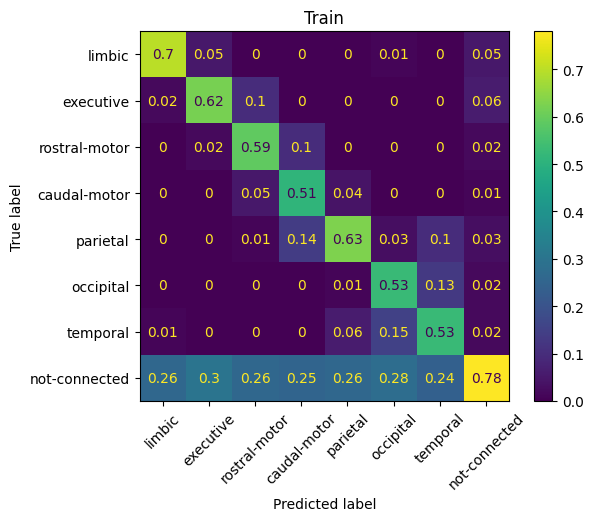
\includegraphics[width=\textwidth]{con_mat_prec_train}
\end{subfigure}
\hfill
\begin{subfigure}{0.49\textwidth}
  \centering
  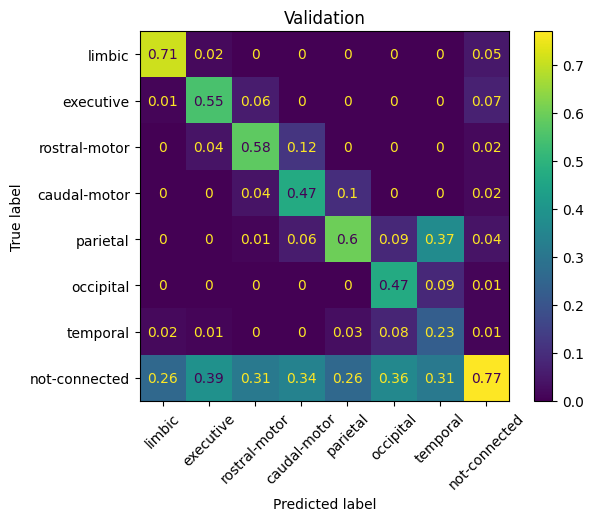
\includegraphics[width=\textwidth]{con_mat_prec_val}
\end{subfigure}
\begin{subfigure}{0.49\textwidth}
  \centering
  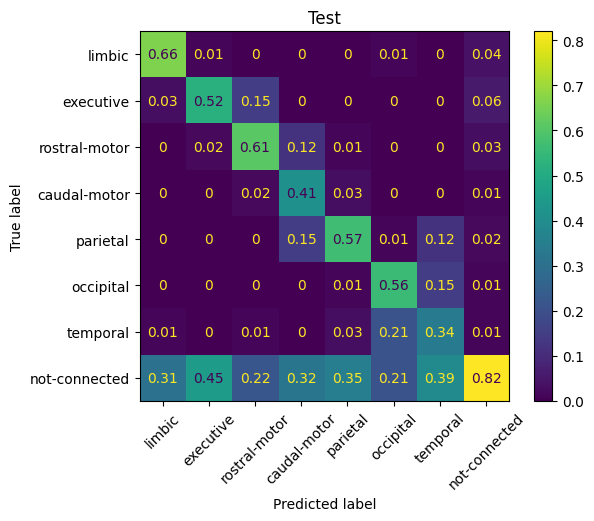
\includegraphics[width=\textwidth]{con_mat_prec_test}
\end{subfigure}
\caption{Confusion Matrices (Precision): Relative Connectivity}
\label{fig:conf_prec}
\end{figure}

These matrices also tell that not all labels are performing equally. As the model clearly struggles with the recall of 'temporal' target region datapoints.

\begin{figure}[H]
\centering
\begin{subfigure}{0.49\textwidth}
  \centering
  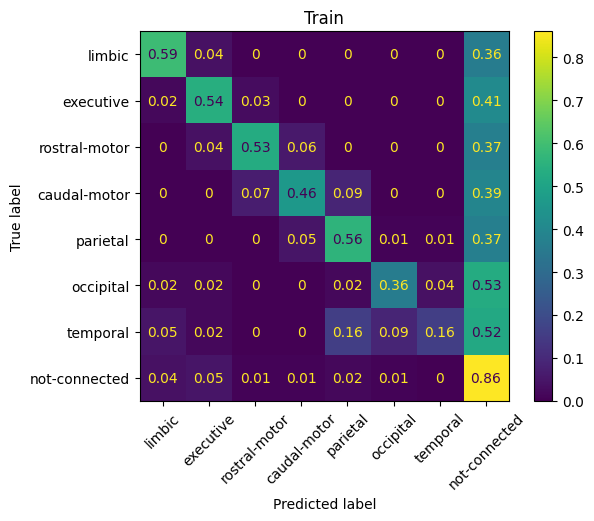
\includegraphics[width=\textwidth]{con_mat_rec_train}
\end{subfigure}
\hfill
\begin{subfigure}{0.49\textwidth}
  \centering
  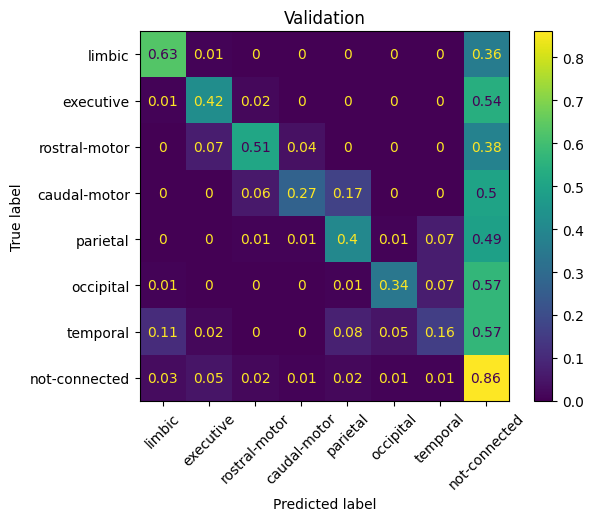
\includegraphics[width=\textwidth]{con_mat_rec_val}
\end{subfigure}
\begin{subfigure}{0.49\textwidth}
  \centering
  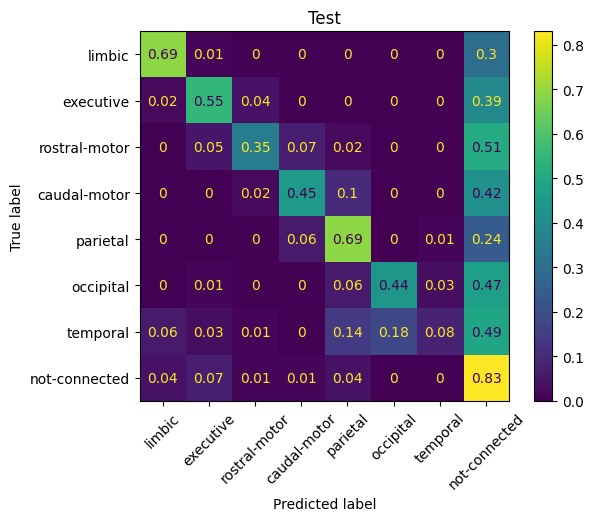
\includegraphics[width=\textwidth]{con_mat_rec_test}
\end{subfigure}
\caption{Confusion Matrices (Recall): Relative Connectivity}
\label{fig:conf_rec}
\end{figure}

\begin{figure}[H]
\centering
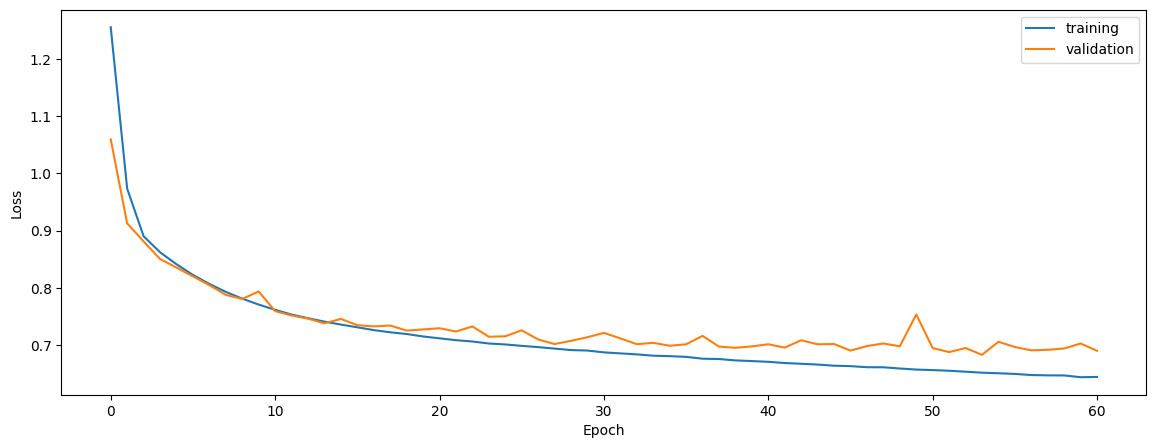
\includegraphics[width=0.7\textwidth]{con_curve}
\caption{Training Curve: Relative Connectivity}
\label{fig:curve-con}
\end{figure}

\begin{figure}[H]
\centering
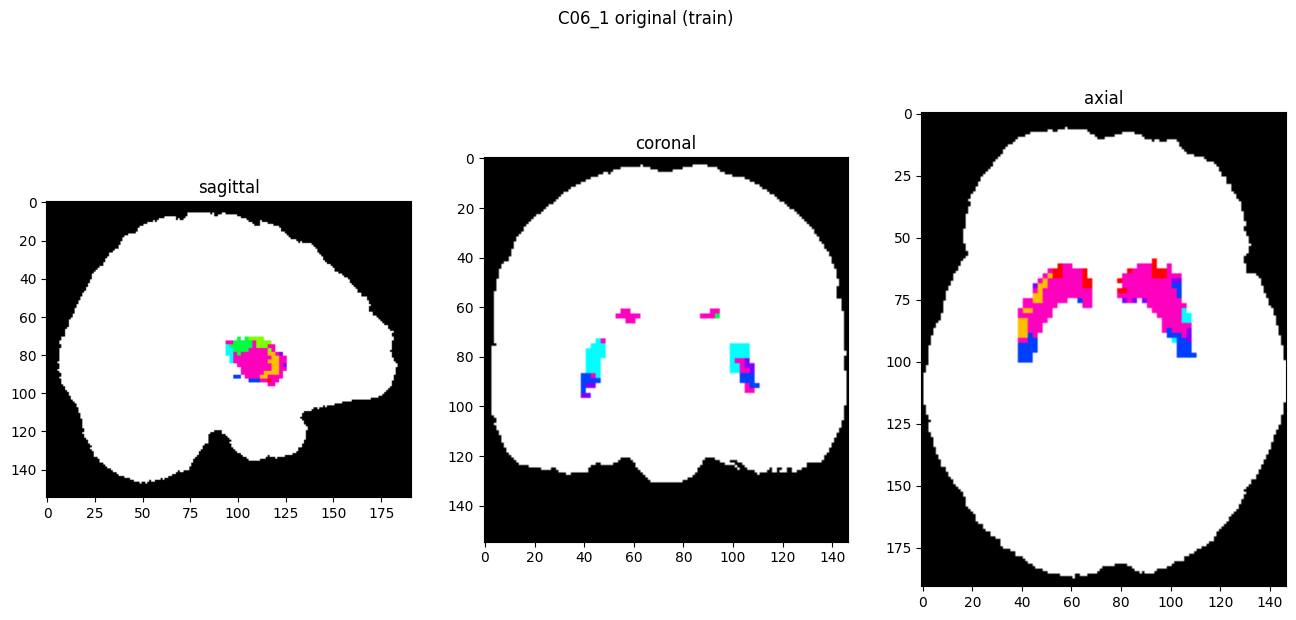
\includegraphics[width=0.65\textwidth]{con_train_o}
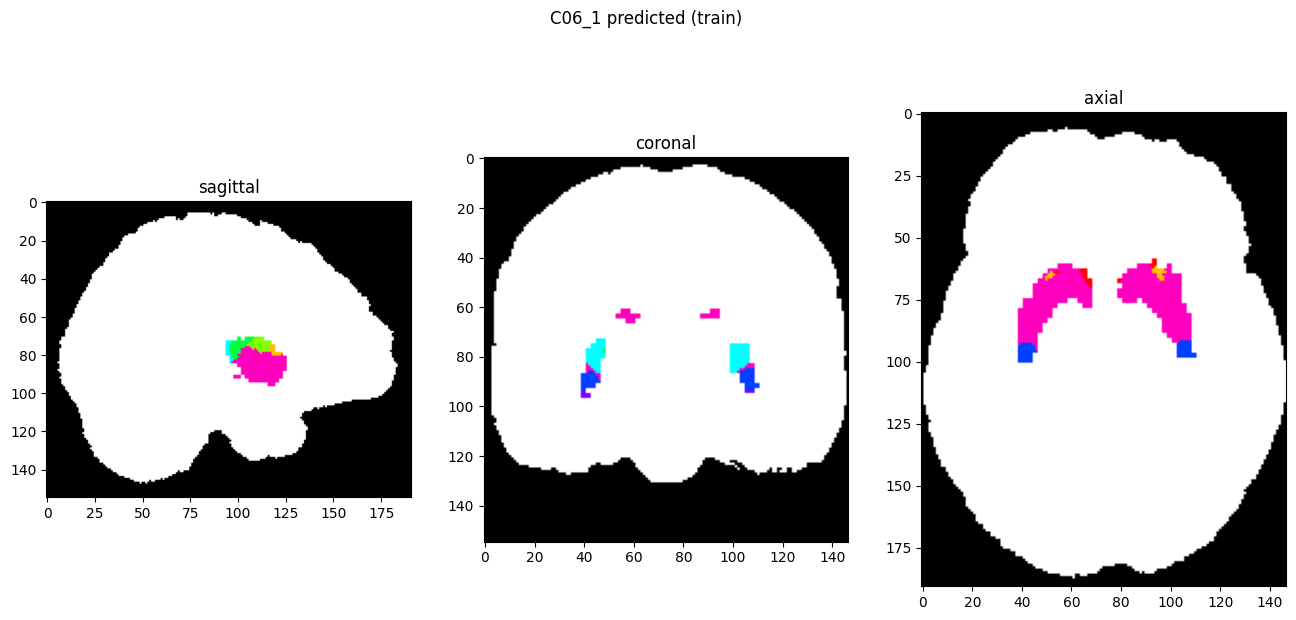
\includegraphics[width=0.65\textwidth]{con_train_p}
\caption{Train Predictions: Relative Connectivity}
\label{fig:pred-tra-con}
\end{figure}

\begin{figure}[H]
\centering
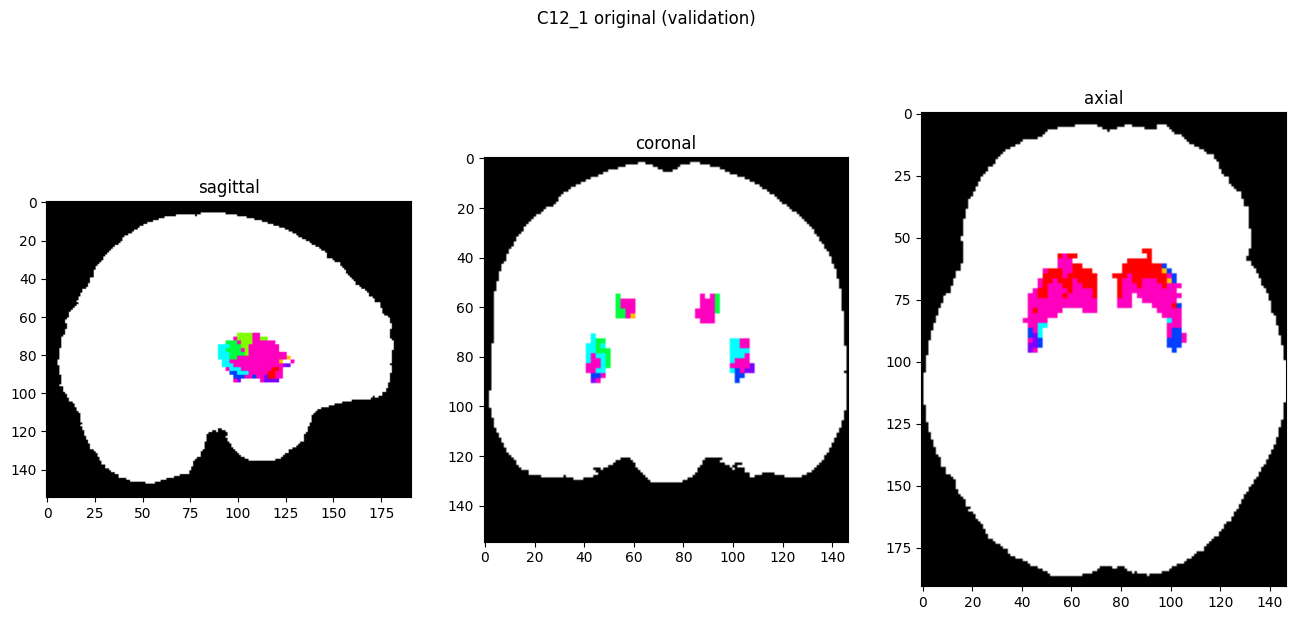
\includegraphics[width=0.65\textwidth]{con_val_o}
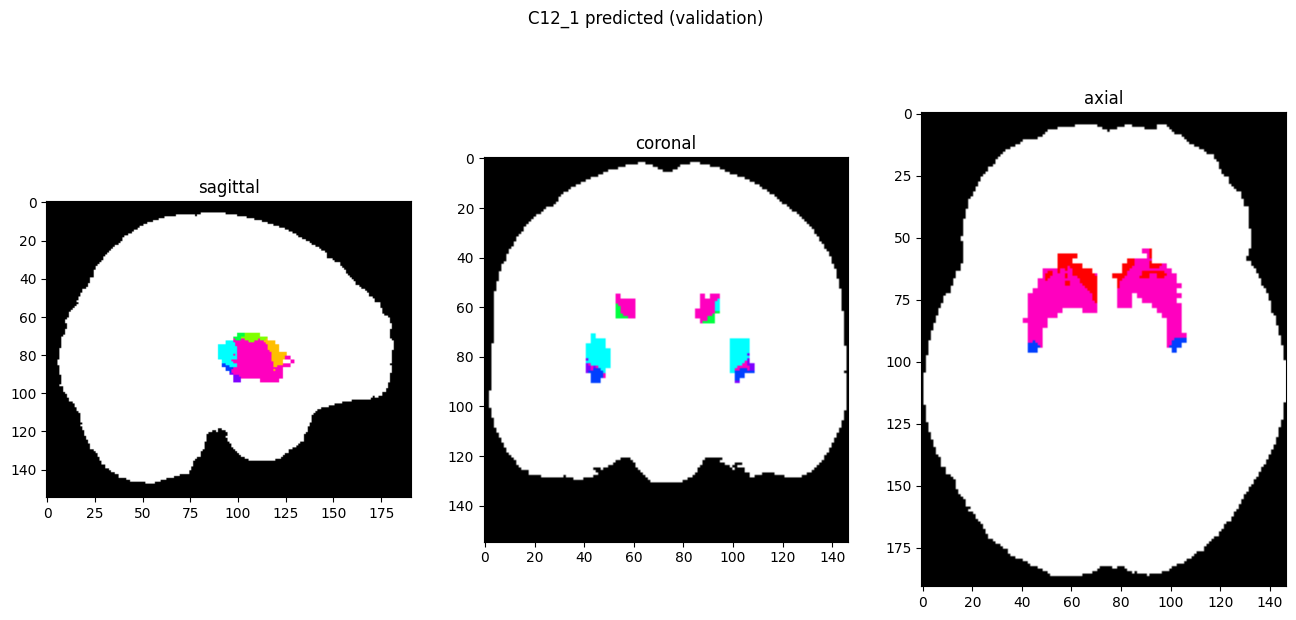
\includegraphics[width=0.65\textwidth]{con_val_p}
\caption{Validation Predictions: Relative Connectivity}
\label{fig:pred-val-con}
\end{figure}

\begin{figure}[H]
\centering
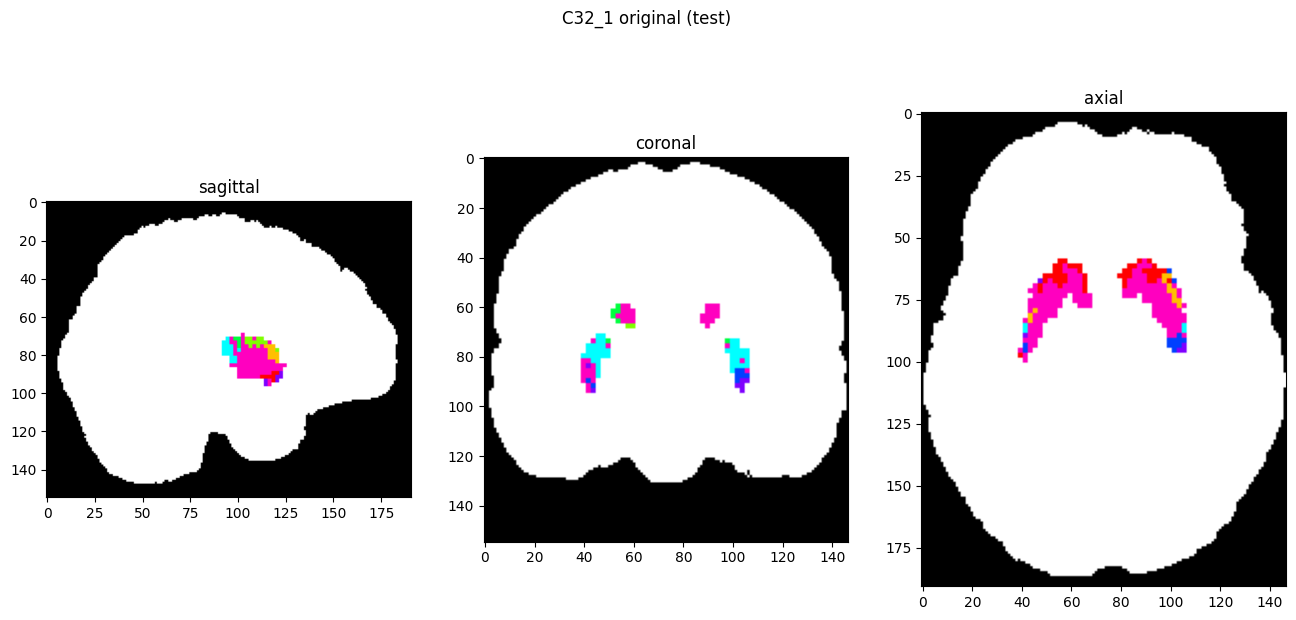
\includegraphics[width=0.65\textwidth]{con_test_o}
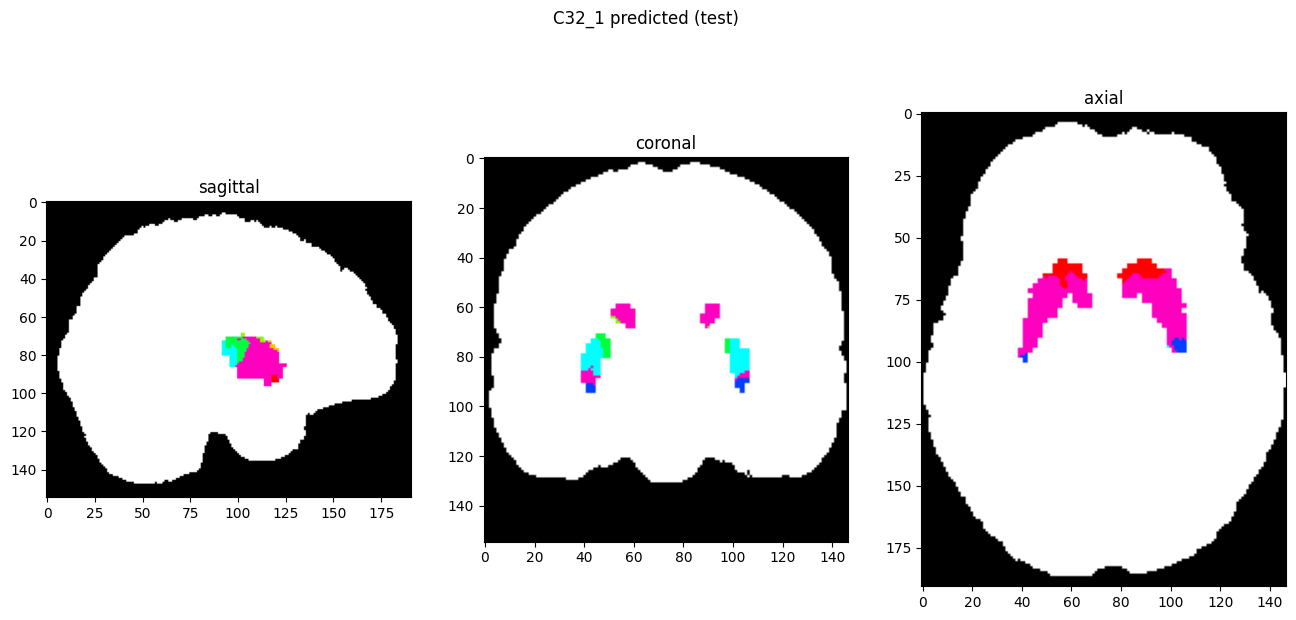
\includegraphics[width=0.65\textwidth]{con_test_p}
\caption{Test Predictions: Relative Connectivity}
\label{fig:pred-tes-con}
\end{figure}

\subsection{Exhaustive Sequential Backwards Feature Selection}
\label{sec:seqback}

Exhaustive sequential backwards feature selection concerns training the model iteratively by removing a single feature at a time, going through all features. After an iteration is completed, the best performing model is chosen, and the corresponding feature is permanently removed before the next iteration, where the model goes through the remaining $n-1$ features.\par
The stopping criterion can be varied from setup to setup, but, in this case, the evaluation metric was chosen to be the raw accuracy, using as a stopping point that where all runs in the iteration performed worse than the baseline (the model with all features included) by more than 2\%.\par
Feature selection was only ran for the Relative Connectivity Segmentation problem, due to it being time consuming and computationally intensive, given the time constraints of the thesis development. This was executed on a network cluster, where the cluster head would give out tasks (a task being a model to train with a set of features to exclude), and the workers would return the validation accuracy.\par
Two logistical oversights that were not mitigated in time were incurred. The first mistake being that the execution of the feature selection was rushed due to the longevity of the task, and the rest of the hyperparameters (besides the excluded features) were chosen before finishing the basic experimentation. And the second being an indirect consequence to it being rushed: the usage of a defective code for balancing the data, where the bug was found only after already executing the feature selection.\par
Due to these mistakes, the selected features turned out not to be very efficient with the final hyperparameters. The feature selection was not executed again due to time and resource limitations. More information detailing this mistake and oversight can be found in the \reflink{sec:improve}{Future Improvements} subsection.\par
Nevertheless, the expected result of re-running the feature selection would be something similar to the current sub-optimal result, where around one third of the features could be excluded before stopping and a maximum increase of 2\% obtained in validation accuracy. The first features to be excluded (See \reflink{tab:sbf}{Table}) were predominantly from the first order radiomics feature class, followed by the \ac{GLCM} radiomics feature class.

\begin{longtable}[H]{|l|l|l|}
\hline
\textbf{Iteration} & \textbf{Excluded Feature} & \textbf{Accuracy} \\ \hline
0. & BASELINE & 59.0 \\ \hline
1. & firstorder\_MeanAbsoluteDeviation & 59.6 \\ \hline
2. & firstorder\_Entropy & 59.9 \\ \hline
3. & firstorder\_Energy & 58.7 \\ \hline
4. & glszm\_SmallAreaLowGrayLevelEmphasis & 58.5 \\ \hline
5. & firstorder\_90Percentile & 59.3 \\ \hline
6. & glcm\_Autocorrelation & 59.5 \\ \hline
7. & firstorder\_Mean & 59.4 \\ \hline
8. & firstorder\_Maximum & 59.1 \\ \hline
9. & glszm\_LowGrayLevelZoneEmphasis & 58.9 \\ \hline
10. & glcm\_Imc1 & 60.0 \\ \hline
11. & firstorder\_Median & 60.1 \\ \hline
12. & glszm\_ZoneVariance & 59.3 \\ \hline
13. & firstorder\_TotalEnergy & 58.9 \\ \hline
14. & firstorder\_10Percentile & 60.4 \\ \hline
15. & firstorder\_Minimum & 59.1 \\ \hline
16. & glszm\_SmallAreaHighGrayLevelEmphasis & 59.9 \\ \hline
17. & firstorder\_InterquartileRange & 60.0 \\ \hline
18. & firstorder\_Kurtosis & 59.6 \\ \hline
19. & firstorder\_RobustMeanAbsoluteDeviation & 59.3 \\ \hline
20. & firstorder\_RootMeanSquared & 59.8 \\ \hline
21. & gldm\_LargeDependenceEmphasis & 58.9 \\ \hline
22. & firstorder\_Variance & 59.1 \\ \hline
23. & glcm\_DifferenceAverage & 59.4 \\ \hline
24. & firstorder\_Uniformity & 58.9 \\ \hline
25. & firstorder\_Skewness & 59.0 \\ \hline
26. & firstorder\_Range & 58.6 \\ \hline
27. & glcm\_JointAverage & 58.7 \\ \hline
28. & glcm\_ClusterProminence & 59.2 \\ \hline
29. & glcm\_ClusterTendency & 58.5 \\ \hline
30. & glcm\_ClusterShade & 60.2 \\ \hline
31. & glcm\_Correlation & 60.0 \\ \hline
32. & glcm\_DifferenceEntropy & 58.1 \\ \hline
33. & glrlm\_RunVariance & 59.3 \\ \hline
34. & glcm\_JointEnergy & 59.6 \\ \hline
35. & glcm\_Contrast & 60.5 \\ \hline
36. & glcm\_Idm & 59.3 \\ \hline
37. & glcm\_Imc2 & 58.7 \\ \hline
38. & glcm\_DifferenceVariance & 59.2 \\ \hline
39. & glcm\_Idmn & 58.0 \\ \hline
40. & glcm\_MCC & 57.9 \\ \hline
41. & glcm\_JointEntropy & 56.6 \\ \hline
\caption{Feature Selection}
\label{tab:sbf}
\end{longtable}

\subsection{Streamline Regression}

An alternative analytical approach would be to try predicting the raw streamline images, and then processing the predictions in the same way the relative connectivity labels were computed in the first place. This method could result in a more robust solution for predicting the upstream data, before preprocessing.\par
Training seven expert models for the seven streamline images (for each cortical target), with the same hyperparameters as the best performing model from the relative connectivity segmentation yielded underwhelming results, with the computed accuracies being 65.1/65.3/63.8, and very low precision/recall for all labels (except the ’not connected’), which is explained by the predicted labels mainly being ’not connected’, in any case. This approach was not explored further in depth due to limited time and resources.





\chapter{Sustainability}
\section{Environmental Aspect}

\subsection{Developement}

The biggest environmental impact of this project was the required computational power to train the models. During the entire duration of the project there approximately a total of 5000 models were trained.\par
Out of which the most demanding part was the exhaustive sequential backward feature selection, which in itself required the training of 3000 models. The return value of this computation is close to none, as it did not increase the model performance. The only marginal benefit is the model being able to reach the same performance on $2/3$rd of the original feature count. This is marginal because the omitted features belong to different feature groups, and the biggest overhead for most feature groups is calculating the voxel-based matrix volume; meaning if not all features are omitted from a feature group, it only decreases the computational requirements marginally. In conclusion, this was not worth computing.\par
The 3000 models trained for the features selection were trained on a wide variety of GPUs in a network cluster. These GPUs were H100, P40, RTX3060, RTX3090, RTX2080, multiple T4s (Google Collab's), multiple P100s (Kaggle's). Mining the cluster head's log, reveals that around half of these models were trained on the H100 and the other half on the rest. The H100 was consuming around 300 Watts of power while training with a speed of 5s/epoch and taking 30-60 epochs on average to stop. The H100 consumed between $1500 \cdot 0.3$kW $ \cdot 30 \cdot 5$s $ \div 60 \div 60 = 18.75$kWh on the lower and $2 \cdot 18.75 = 37.5$kWh on the upper end. The other half is harder to estimate due to the many different GPUs used in the cluster, but a crude estimate is $1500 \cdot 0.2$kW $ \cdot 30 \cdot 8$s $ \div 60 \div 60 = 20$kWh on the lower and $2 \cdot 20 = 40$kWh on the upper end. Rounding the sum of them up to $80$kWh and adding an extra $30\%$ overhead for running the rest of the components of the servers/PCs, results in an upper boundary of $104$kWh consumed during the feature selection.\par
The rest of the 2000 models were trained on the P40 and RTX3060, with preferring the P40 and probably training $3/4$th of them. Doing the same estimations for the P40 yields $1500 \cdot 0.2$kW $ \cdot 30 \cdot 7$s $ \div 60 \div 60 = 17.5$kWh on the lower and $2 \cdot 17.5 = 35$kWh on the upper end. And for the RTX3060 yields $500 \cdot 0.15$kW $ \cdot 30 \cdot 7$s $ \div 60 \div 60 = 4.375$kWh on the lower and $2 \cdot 4.375 = 8.75$kWh on the upper end. Rounding the sum of them up to $45$kWh and adding an extra $30\%$ overhead for running the rest of the components of the server, results in an upper boundary of $58.5$kWh consumed during the the rest of the trainings.\par
Feature extraction was running on a CPU, with the entire server consuming 200 Watts during the process. The entire duration while feature extraction was running is around 2 weeks. The total power consumption of the feature extraction was $0.2$kW $ \cdot 14$d $ \cdot 24$h $ = 67.2$kWh.\par
In summary this project had the following environmental impact, calculating with the average of \citelink{kwhprice}{$0.25$€/kWh for the price of the electricity} and \citelink{carbon}{$0.2$kgCO$_{2}$e/kWh for the emission}:
\begin{table}[H]
\centering
\begin{tabular}{|l|l|l|l|}
\hline
\textbf{Part} & \textbf{Consumption} & \textbf{Price} & \textbf{Emission} \\ \hline
feature selection & $104$kWh & $26$€ & $20.8$kgCO$_{2}$e \\ \hline
rest of the experiments & $58.5$kWh & $14.6$€ & $11.7$kgCO$_{2}$e \\ \hline
feature extraction & $67.2$kWh & $16.8$€ & $13.4$kgCO$_{2}$e \\ \hline
\textbf{Total} ($+10\%$ overhead; rounded up) & $260$kWh & $65$€ & $52$kgCO$_{2}$e \\ \hline
\end{tabular}
\caption{Sustainability}
\label{tab:sus1}
\end{table}
For reference, this number is a bit less than the \citelink{kwhavg}{average Spanish household's monthly power consumption of $324$kWh.}

\subsection{Production}
\label{sec:susprod}

This project, whether implemented in a production, clinical or research setting, has the potential to significantly enhance sustainability in its respective fields. Acquiring \ac{DTI} data typically requires up to 40 minutes, depending on the specific parameters, whereas obtaining a T1 image takes only about 8 minutes, making data acquisition a considerable time-saving step. Additionally, \ac{DTI} data demands extensive and labor-intensive preprocessing. \textbf{Accelerating clinical or research workflows by a factor of 5} not only saves time but also increases the capacity for data collection or patient processing by the same factor.\par
Synthesizing a single record of relative connectivity or diffusion \ac{FA}/\ac{MD} takes only a few seconds on a GPU and the radiomic feature extraction takes around 20 minutes beforehand. This translates into the approximate energy demand of $200$W $ \cdot (5$s $ \div 60 + 20$m$) \div 60 = 67$Wh of synthetizing a record. It can be argued that the time saved with the data acquisition is lost with the time it takes to extract the radiomic features, but neither the doctor (or MRI operator) and patinet needs to be present during the computation of the feature extraction. Assuming an MRI machine has a \citelink{kwhmri}{consumption of $25$-$70$kW} and calculating with an average of $50$kW, adds up to the power requirement of $50$kW $ \cdot 40$m $ \div 60 = 33.3$kWh per \ac{DTI} record. Adding up the total energy requirements of T1 data acquisition and record synthesis is $50$kW $ \cdot 8$m $ \div 60 + 67$Wh $ \div 1000 = 6.7$kWh per record. This means that \textbf{this method could be 5 times more sustainable than the traditional approach}. And it would return the energy consumption of the development phase in the data acquisition of $260 \div (33.3 - 6.7) = 10$ records, which is naturally a miniscule number compared to how many MRI records are being done in the world.

\section{Economic Aspect}

\subsection{Cost}

The electricity cost during the development phase amounted to $65$€. Approximately half of this cost was covered by colleagues and their networks, who contributed computational resources during the feature selection process. Additional support came from free services provided by Google and Kaggle.\par
Realistically, billing this project would consist of three components: the cost of labor, the price of the server used for development, and the electricity consumed. With the electricity cost already detailed, the server cost and labor are interconnected. The project could have been executed on a less powerful machine, though this would have required more time and more careful focus on software design. Throughout the development, the primary limiting factors were RAM and disk storage. Significant effort was invested in developing efficient data structures and optimizing the memory footprint to address these constraints.\par
In conclusion, the minimum hardware which this project could be feasibly executed on is 32GBs of RAM, Intel Core i5-12600K (or similar), Nvidia RTX3060 (or similar), and $256$GBs of storage. The current cost (new parts ordered from Amazon) of such server (with 'cheap' consumer grade hardware) would be around $300$€ for the GPU, $150$€ for the CPU, $50$€ for the RAM, $25$€ for the SSD, and $150$€ for the motherboard, adding up to $675$€. The main limiting factors in this configuration are the RAM, which was utilized up to $128$GBs during development; and disk storage, which was utilized up to $300$GBs. The extra RAM and storage would cost an additional $200$€ and $25$€ totalling at a new sum of $900$€.\par
The development of this project required approximately $500$ hours of work. Calculating with the \citelink{salary}{average hourly rate of a software engineer in Spain} of $19$€, leads to a total labor cost of $19$€ $ \cdot 500$h $ = 9500$€. Therefore, the total billing for the project would be:
\begin{table}[H]
\centering
\begin{tabular}{|l|l|l|l|}
\hline
\textbf{Part} & \textbf{Price} \\ \hline
Cumulative Salary & $9500$€ \\ \hline
Server Components & $900$€ \\ \hline
Electricity & $65$€ \\ \hline
\textbf{Total} & $10465$€ \\ \hline
\end{tabular}
\caption{Billing}
\label{tab:sus2}
\end{table}

\subsection{Return}

This project by all means is a proof of concept, checking the viability of this approach. More information on the exact conclusions are in \reflink{sec:conclusions}{chapter}, but the potential return value of this project is huge.\par
As stated in the previous \reflink{sec:susprod}{subsection}, this project has the potential to accelerate the clinical and/or research workflows by a factor of 5. The economic implications are applicable for both clinical and research workflows. In the clinical workflow, \textbf{this could increase the number of patients processed by a factor of 5}, with minimal extra cost. Especially compared to the alternative of buying 4 additional MRI machines, and hiring operators for them. In a research workflow it probably has less of an economic impact, but more of a logistical impact. As it could simplify the data acquisition, thus \textbf{allowing researchers to have up to 5 times more data acquired} with minimal extra resources invested. But even more importantly it opens the door of processing past anatomical MRI records, as they are much more common than dMRI records, virtually \textbf{increasing the available data for researchers by several magnitudes} (depending on the exact application of course).

\section{Social Aspect}

\subsection{Development and Collaborations}

The development of the project mainly required collaboration from Estela Camara Mancha (external thesis supervisor and project originator) and Alfredo Vellido Alcacena (internal thesis supervisor). Estela being the project originator, this project demanded her time the most, in the neighborhood of 40-50 hours \textcolor{red}{TODO}. Alfredo mostly helping with the formalities and miscellaneous nuances, had a demand of 10-15 hours \textcolor{red}{TODO} of his time. Additionally Estella's colleague Vasiliki Bikou also spent a good chunk of her time on catching me up to speed with the contextual information of the project. And lastly my good friends Botond Lovasz, Andris Gyori and Daniel Csepregi-Horvath donated computational power, and required a few hours of their time to set up the worker nodes on their hardware. I especially want to thank Botond for using his connections and giving me access to the H100 state of the art tensor core GPU.

\subsection{Inclusivity}
\label{sec:inclusive}

The most obvious consideration from age, gender, sex, and cultural diversity; is sex, as \citelink{sexbrain}{males and females have slightly different brain structures}. For the used control records, there are 17 male and 15 female records, which is a relatively even split; and for the patient records, there are 25 male and 13 female records, which is a bit unbalanced. This theoretically could negatively impact the under represented group if there are truly any differences between the two sexes that matter from the model's perspective. However in the case of the project due to the very limited number of records, it was not an option to discard 1/3rd of the patients, to have the sexes completely balanced. And it would also need further experimentation to determine if this truly impacts this project or not.\par
This potential difference was overlooked during most of the project's lifetime, but it should have been included as another constant ratio to be kept during the train/validation/test splitting, which was covered in \reflink{sec:travaltes}{subsection}. Due to limited time and resources, the models will not be re-trained with this new rule in mind, and this is something that will be included in the \reflink{sec:improve}{Future Improvements} subsection.\par
The rest of the considerations are less pressing and hard to take into account, like the brain structure of different ethnicities is an under researched area, plus this dataset does not contain any information regarding this aspect. The only other consideration which can be related is age, but this is partially accounted for as part of the constant symptomatic/asymptomatic ratio. Because being symptomatic is closely related to the \ac{CAP} score (covered in \reflink{sec:clinical}{subsection}), which is directly related to age. Thus symptomatic/asymptomatic is indirectly related to age.

\section{Risks}

Environmental, Economic and Social risks are not really applicable to this project, as it is a foundational proof of concept research project.









\chapter{Conclusions}
\label{sec:conclusions}

This foundational project has huge potential thanks to the possible return and applications of the used approach. Due time and resource limitations, the experiments only focused on the Basal Ganglia, so by no means any of the performance metrics prove that a generalized solution is viable. However the \ac{FA} and \ac{MD} predictions are really promising, and would be interesting to see how would it perform on the entire brain, and not just the \ac{ROI}. On the other hand the Relative Connectivity predictions are not even nearly precise enough to call them usable, but admittedly the labels themselves will inherently contains quite a bit of noise, due to the very sensitive process extracting the labels with tractography.\par
This project only delved into a tiny fraction of the endless sea of possible preprocessing approaches, and it only experimented with some very basic model architectures. Nevertheless, the viability of this approach and hypothesis is not disproven, but it definitely needs some new ideas implemented to make it work.\par

\section{Future Improvements}
\label{sec:improve}

As mentioned in \reflink{sec:seqback}{subsection}, there was a serious oversight during the execution of the exhaustive sequential backwards feature selection. At the time it was believed that the model was performing better on balanced data, due to a bug in the code. Thus, all of these models are performing much worse than the models during the experimentation. The bug was fixed, but due to limited time and resources the feature selection was not executed again.\par
Further investigating the sex imbalance issue discovered in \reflink{sec:inclusive}{subsection}, reveals that with the used seed for the experimentation is not terribly imbalanced for the most part, but there are definitely room for improvement by enforcing a constant ratio. The male/(male+female) ratio for the control record splits are $0.49$/$0.67$/$0.67$ (train/validation/test), and for the patient records are $0.62$/$0.5$/$1$.\par
Besides these known mistakes, there are some issues that are hard to quantify. For example due to the different imaging of the anatomical records and the \ac{DTI} record, even after a perfect affine registration they can have tiny misalignments. Explained by the records being taken separately, possible physiological movements, and independent preprocessing steps. This may be the reason behind the normalized experiments performing better than the native experiments in most cases, as the normalized images have less discrepancy between them.\par
Additionally, one aspect was not investigated thoroughly during this project and that being the kernel size, binning parameters, and feature class relationships, during the voxel based feature extraction. For the sake of simplicity, only a unified binning method was used for all kernel sizes and all feature classes. But logically the binning parameters could be optimized for each kernel size and feature class. For example logically the \ac{GLRLM} feature class could yield fundamentally different features even just by adjusting the bin size a tiny bit at large kernel sizes.\par
Selecting the most efficient kernel size combinations were not investigated thoroughly either. Due to limited resources, the maximum kernel size used was 21, but there were no reason to stop here (besides to be able to finish this project in time).\par
Ultimately, even with the 'few' simple aspects that were taken into consideration during this project, the hyperparameter space is gigantic and some compromises were had to be made. After investing over 500 hours into this project, the educated guesses for these potential improvements are:
\begin{itemize}
  \item The feature selection should have a marginal improvement on the model performance.
  \item The gender imbalance should not have a measurable impact on the model performance on this scale (with less than 70 available records in total).
  \item The binning parameter optimization for the kernel sizes and feature classes would probably have a big impact on the model performance.
\end{itemize}
And lastly, all experiments should be repeated at least a few times, with different splits and seeds. And the experiments should be evaluated with the means and medians of the model performance indicators, across different runs.

\section{Project Future}

Ultimately there are two paths to continue this project. First, the \ac{FA} and \ac{MD} experiments could be expanded to the entire brain and a generalized model should be developed. And the other being the refinement of the Relative Connectivity experiments, as it definitely need improvements and new ideas.




%TC:ignore
\printbibliography[heading=bibintoc,title={Sources of Information}]
\appendix

\chapter{Software Design}
The software design was mainly guided by the provided format of the raw data, which came from different sources, as different researchers were working with different data at the Hospital, and they did not have a unified collection. Thus, the following documentation of the software design will be structured going from the raw data, to the preprocessed data, and then the model itself.

\section{Raw Data}

The raw data (an example of their contents is found in \reflink{fig:digfilraw}{Figure}) was originally scattered amongst many files, registered in different spaces, and do not have masks applied (this, along with other challenges detailed in \reflink{sec:preproc}{Section}).

\begin{figure}[H]
\centering
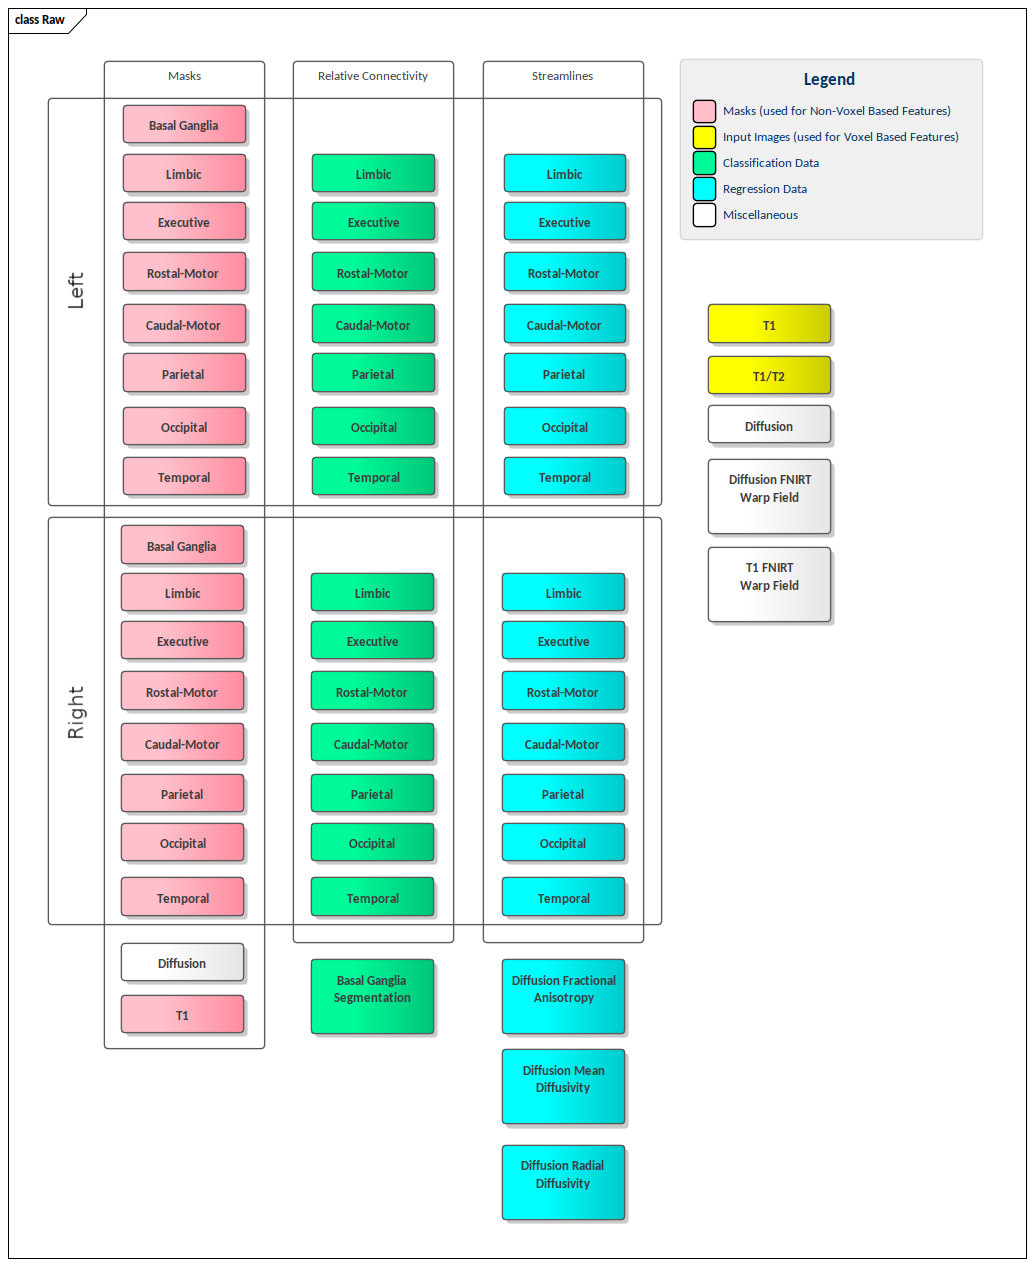
\includegraphics[width=0.692\textwidth]{DataRaw}
\caption{Files: Raw}
\label{fig:digfilraw}
\end{figure}

The class diagram documentations are detailed abstractions of the actual source code, as \ac{UML} is not completely Python-compliant. Before moving on, the simple data types and primitives seen in \reflink{fig:digclstyp}{Figure} are used in the \ac{UML} diagrams:

\begin{figure}[H]
\centering
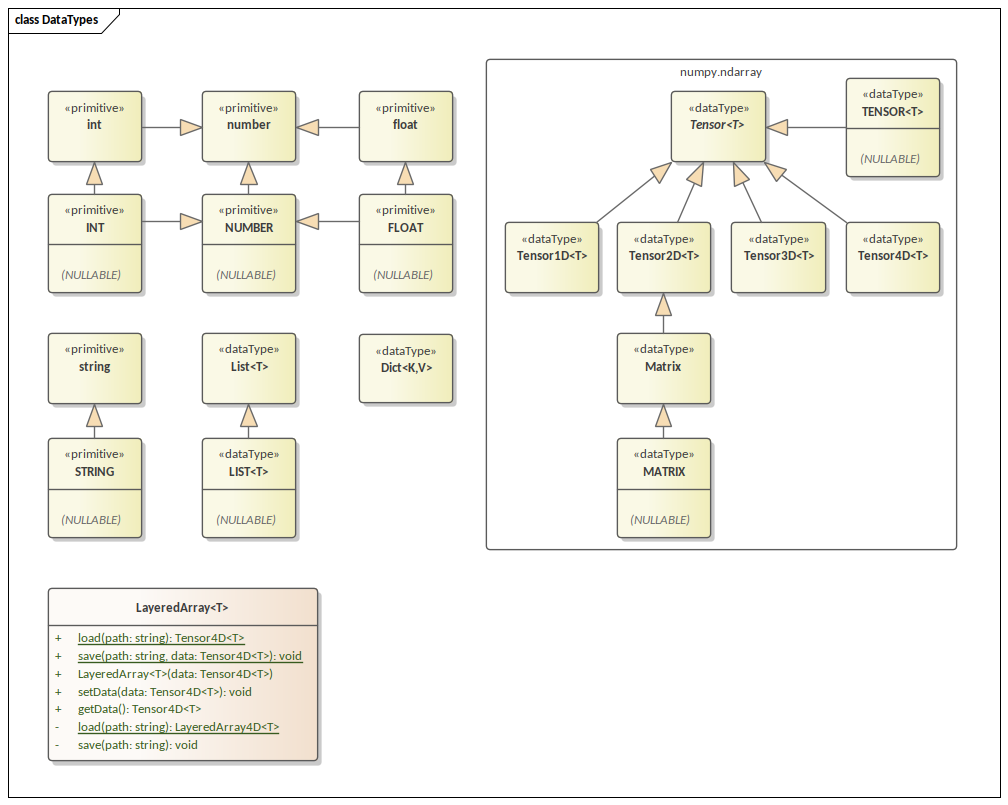
\includegraphics[width=0.8\textwidth]{ClassDataTypes}
\caption{Class Diagram: Data Types}
\label{fig:digclstyp}
\end{figure}

The odd one out in this diagram is the LayeredArray, which is more than a simple data type or primitive. This class is a simple space efficient data structure of a 4D tensor.\par
Storing the raw tensor of some of the data provided can be highly inefficient. Ultimately, the design aims to collect the scattered data from multiple files into clean logical groups: for example, all the cortical target masks into a single 4D tensor, where the 4th dimension is reserved for the multiple targets. This is a greatly inefficient way of storing the data, though, as each target region only takes up a small portion of the entire space. The idea behind the LayeredArray class is that it stores the 4D tensor as a list of 3D tensors, each cropped down to their effective space where there are non-zero voxels. This also requires an additional list of 3D vectors to store each layer's origin, and where to paste it in the original space.\par
This solution offers a very efficient way of storing data for this use case, as the raw storage solution for the cortical target masks involved around 50MBs, and this solution cuts it down to 3MBs. This is even more drastic for the relative connectivity, which is more than a simple boolean mask and proportionally takes up even less space of the entire brain; in which's case it was cut down from 110MBs to 0.5MBs, reducing the disk requirement by several magnitudes.\par
The original \ac{NIfTI} format also does a very good job at storing data efficiently, but this solution provides control over the way of storing the data on a much lower level. This is beneficial as the data are stored in numpy format, making it easier to ignore certain data type safety checks, data type conversions, and leaving behind the \ac{NIfTI} format's additional complexity of the orientation, transformation, and many more nuances that are part of the \ac{NIfTI} header.\par
This has the undoubted drawback of not being able to use \ac{FSL} tools natively on our datatypes, such as fsleyes for simply viewing a record. But thanks to the opensource nature of the \ac{FSL} suite, with a few additional lines of code, support can be added for our datatypes (included in \reflink{apx:source}{Appendix}).

\begin{figure}[H]
\centering
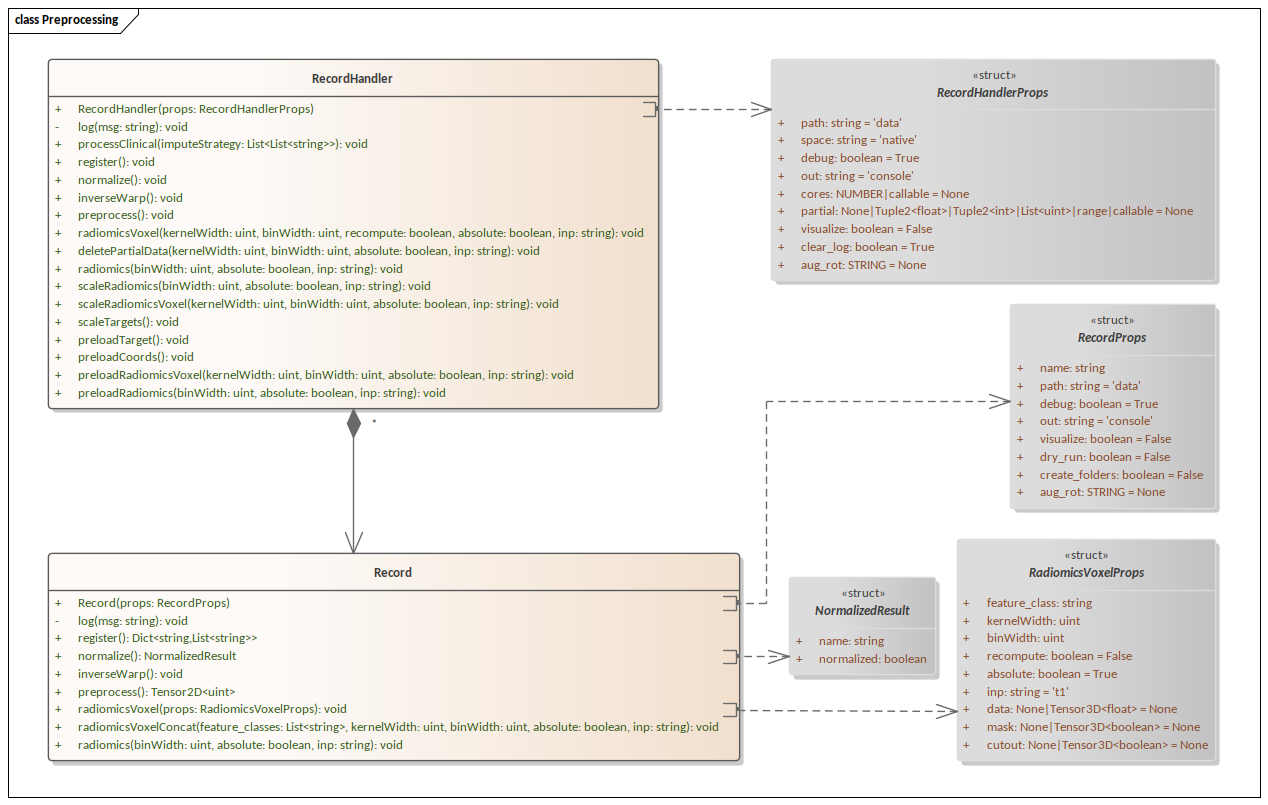
\includegraphics[width=0.95\textwidth]{ClassPreprocessing}
\caption{Class Diagram: Preprocessing}
\label{fig:digclspre}
\end{figure}

The class diagram shown in \reflink{fig:digclspre}{Figure} contains the two classes responsible for the preprocessing of the data. The RecordHandler being the controller itself that handles the high level operations on a collection of records, and the records handling the low level computations on the data itself.

\section{Common Functions}

There is a set of static common functions providing the low level backbone of the entire thesis project. They are grouped into two categories, namely util and visual (as seen in \reflink{fig:digclscom}{Figure}), where the former contains everything from simple data type castings, external \ac{FSL} library system calls, to computing radiomics, and more, and the latter one is a collection of functions for visualizing data.

\begin{figure}[H]
\centering
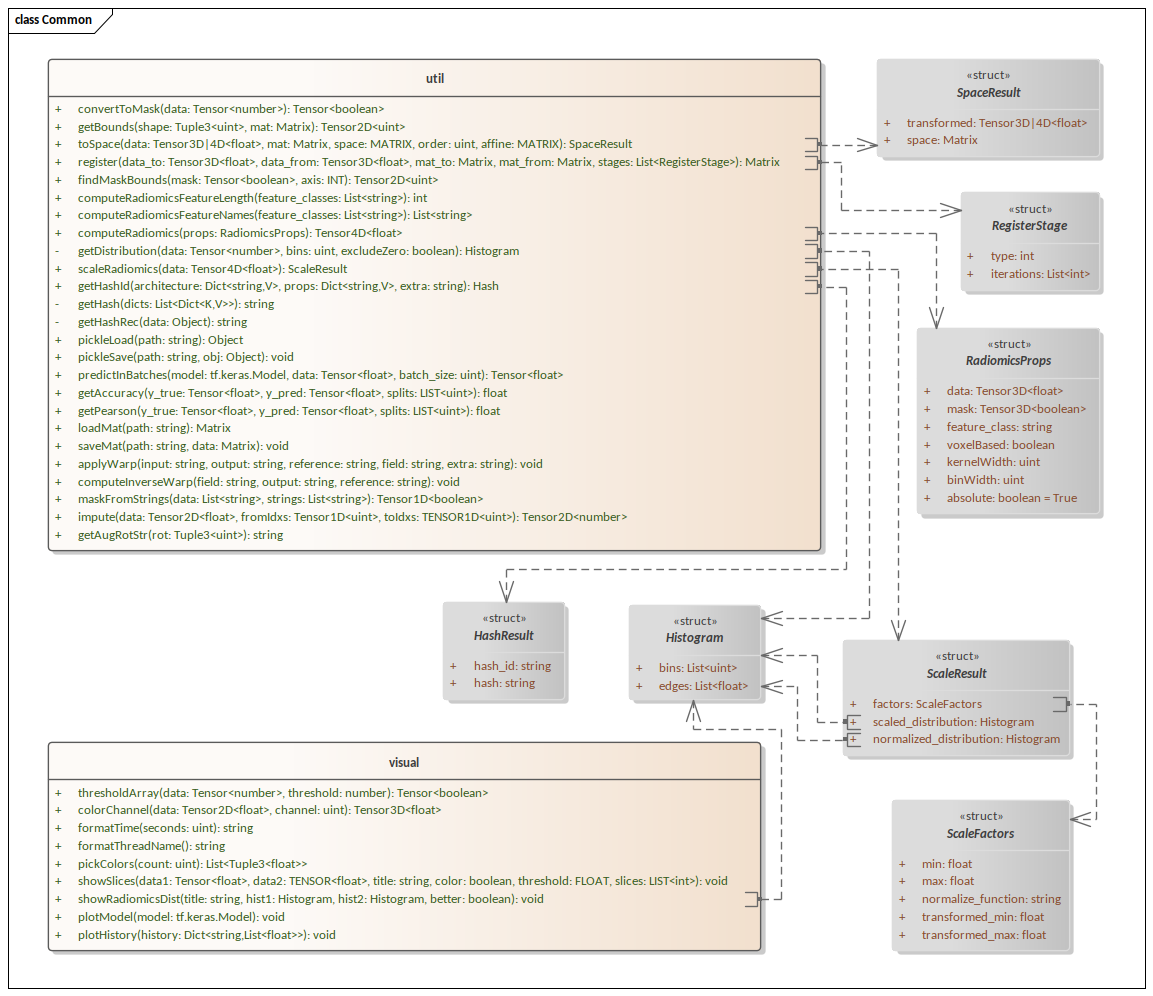
\includegraphics[width=0.95\textwidth]{ClassCommon}
\caption{Class Diagram: Common}
\label{fig:digclscom}
\end{figure}

\section{Preprocessed Data}

Preprocessing the data are composed from the next few high level operations done by the RecordHandler:
\begin{enumerate}
  \item Register some records (not needed for most of them)
  \item Compute all normalized records
  \item Compute the inverse \ac{FNIRT} warp field
  \item Convert native records into our numpy format (apply the affine transformations, merge different sources, etc.)
  \item Compute scaling factors across all native records
  \item Preload native records
  \item Convert normalized records into our numpy format
  \item Compute scaling factors across all normalized records
  \item Preload normalized records
  \item Construct normalized coordinate maps
  \item Warp normalized coordinate maps into native space
  \item Scale and preload coordinate maps
  \item Impute clinical data
\end{enumerate}

After preprocessing, the set of logical groupings and files seen in \reflink{fig:files}{Figure} are left, split into native and normalized records:

\begin{figure}[H]
\centering
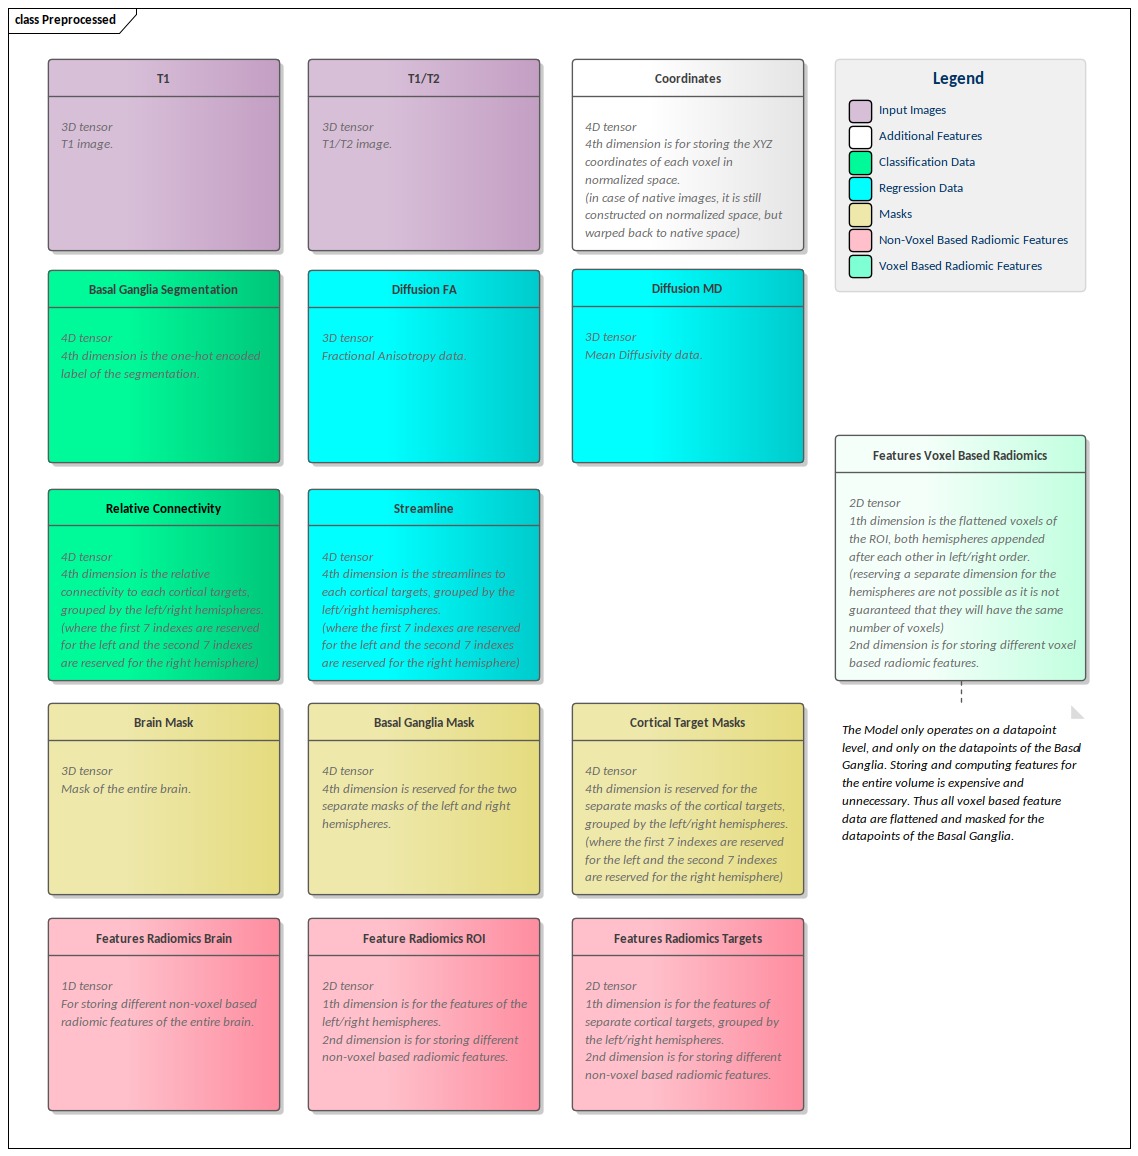
\includegraphics[width=0.85\textwidth]{DataPreprocessed}
\caption{Files: Preprocessed}
\label{fig:files}
\end{figure}

\section{Data Generator}

As this thesis project focuses only on the voxels inside the Basal Ganglia, this means that the model is never going to operate outside of that volume at a datapoint level.

\begin{figure}[H]
\centering
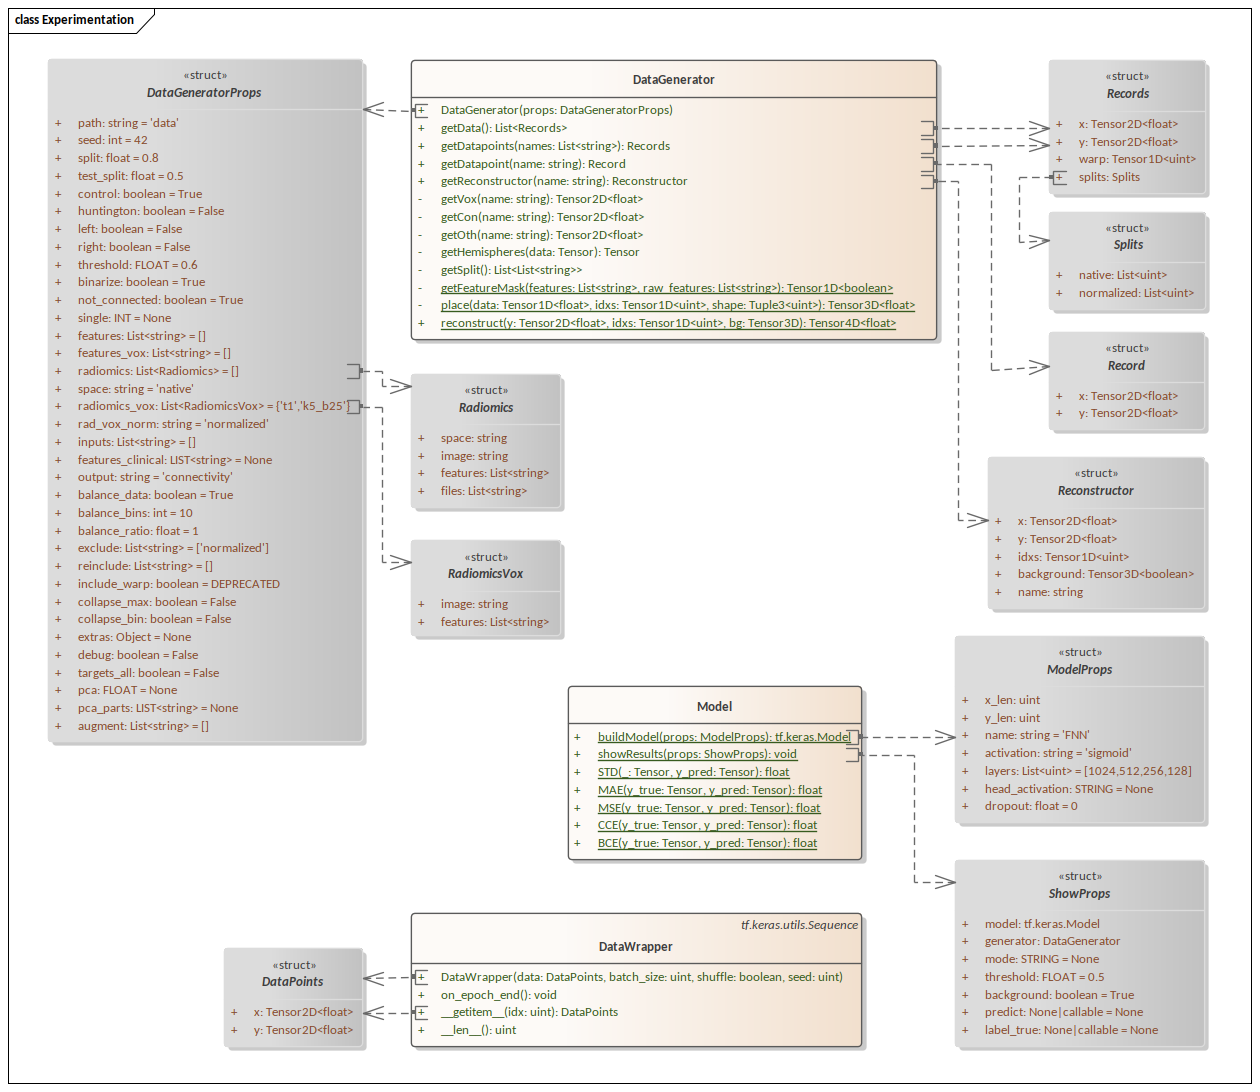
\includegraphics[width=0.95\textwidth]{ClassExperimentation}
\caption{Class Diagram: Experimentation}
\label{fig:digclsexp}
\end{figure}

The DataGenerator class is responsible for feeding the Model with data, according to the specifications of the experiments (a schematic representation of them are found in \reflink{fig:digclsexp}{Figure}). In order to make this more efficient and fast, loading the entire volume of records from disk can be avoided by 'preloading' the \ac{ROI} from each record. This simply put means that all logical grouping and files specified in \reflink{fig:files}{Figure} are preloaded into 1D and 2D tensors, where the first dimension is the flattened voxels of the \ac{ROI} and the second is whatever layers were stored originally in the last dimension of the spatial data (for example the streamlines of the different traget regions).\par
Computing and persisting the preloaded data vastly speeds up the DataGenerator. Although this has the added consequence that the preloaded data yields a pair of tensors instead of a single volume, as there is differentiation between the left and right hemispere datapoints. And the voxel count in the two hemispheres are not symmetrical, thus the hemisphere differentiation can not be stored as an extra dimension. A design decision was made to store the left and right hemisphere data in separate files.\par
The properties of the DataGenerator provided in its constructor, as listed in \reflink{tab:datagenprops}{Table}, define the type and format of the generated data.

\begin{longtable}[H]{|L{3cm}|L{3cm}|L{10cm}|}
\hline
\textbf{Value} & \textbf{Type} & \textbf{Description} \\ \hline
path & string & path of the data \\ \hline
seed & int & random seed for the train/val/test splits \\ \hline
split & float & train/all ratio \\ \hline
test\_split & float & test/(test+validation) ratio \\ \hline
control & boolean & include control records \\ \hline
huntington & boolean & include huntington records \\ \hline
left & boolean & include left hemisphere datapoints \\ \hline
right & boolean & include right hemisphere datapoints \\ \hline
threshold & FLOAT & if not None it thresholds the labels by setting the values under the provided threshold to zero; if 0 it re-one-hot encodes the labels (sets the maximum label to 1 and the rest to 0) \\ \hline
binarize & boolean & if thresholded and True, it also sets the labels above the threshold to 1 (and the rest to 0) \\ \hline
not\_connected & boolean & if thresholded and True, it appends an additional 'not connected' label, which complements the sum of the labels per voxel to 1 \\ \hline
single & INT & if not None it only returns the label with the provided index \\ \hline
features & List$<$string$>$ & used non-voxel based radiomics features (emptylist means all) \\ \hline
features\_vox & List$<$string$>$ & used voxel based radiomics features (emptylist means all) \\ \hline
radiomics: List$<$Radiomics$>$ & space: string & space of non-voxel based radiomic features \newline (native/normalized) \\ \cline{2-3}
 & image: string & input image of non-voxel based radiomic features \newline (t1/t1t2) \\ \cline{2-3}
 & features: List$<$string$>$ & list of binning settings of the features \newline (b25, b50, b10r... etc.) \\ \cline{2-3}
 & files: List$<$string$>$ & list of region mask settings of the features \newline (targets/roi/brain) \\ \hline
space & string & space of voxel based radiomic features \newline (native/normalized) \\ \hline
radiomics\_vox: List$<$ & image: string & input image of voxel based radiomic features \newline (t1/t1t2) \\ \cline{2-3}
{   }RadiomicsVox \newline$>$ & features: List$<$string$>$ & list of binning and kernel settings of the features \newline (k5\_b25, k9\_b50, k7\_b10r... etc.) \\ \hline
rad\_vox\_norm & string & use normalization, or only min-max scaling on the voxel based radiomic features (norm/scale) \\ \hline
inps & List$<$string$>$ & additional voxel inputs (t1/t1t2/diffusion/diffusion\_fa/ diffusion\_md/diffusion\_rd) \\ \hline
features\_clin & List$<$string$>$ & additional clinical data inputs (empty array means all) \\ \hline
outp & string & output (connectivity/streamline/basal\_seg/ diffusion\_fa/diffusion\_md/diffusion\_rd) \\ \hline
balance\_data & boolean & enables data balancing \\ \hline
balance\_bins & int & number of bins used for continuous data when balancing \\ \hline
balance\_ratio & float & ratio of the resampling of the difference between each bin and the max bin when balancing (where 0 is unbalanced and 1 is perfectly balanced) \\ \hline
exclude & List$<$string$>$ & can manually add missing groups of records to exclude (t1t2/normalized/basal\_seg/diffusion\_fa) \\ \hline
reinclude & List$<$string$>$ & can manually re-include (append) missing groups of records to the train split (t1t2/normalized/basal\_seg/diffusion\_fa) \\ \hline
debug & boolean & only returns 1/1/1 records for train/val/test when True \\ \hline
augment & List$<$string$>$ & list of record suffixes, used to include augmented records in the training split; for example the suffix '\_5\_0\_0' is used for the rotation augmentation of 5, 0 and 0 degrees on the X, Y and Z axis (naturally these records needs to be computed before using here) \\ \hline
\caption{Data Generator Properties}
\label{tab:datagenprops}
\end{longtable}








\chapter{Software Implementation}
\label{app:impl}

Detailing the entire implementation of the project is beyond the scope of this report. But some solutions contain non self explanatory ideas and are worthy of detailed explanations. For more details please refer to the source code.

\section{Interpolation}

One crucial detail concerning the application of transformations to the records is the type of interpolation used. For some images like T1, the standard trilinear interpolation makes sense, as the values in-between voxels should be continuous. However, for some other images like binary masks, the interpolation should be the nearest neighbour, as the edge of the mask cannot be interpreted as a fraction. And most importantly, the relative connectivity and streamline images should also be interpolated with the nearest neighbour. In theory, these images could be computed with trilinear interpolation, but this would degrade the images due to their unbalanced nature of having a few voxels with high intensity values relative to the entire voxel space, effectively eroding the boundaries of the high intensity volumes.\par
In practice this meant using 0th and 1st order spline interpolations, which are numerically the same as nearest neighbour and trilinear interpolations.

\section{Multithreading}

As most of the preprocessing could not be easily offloaded to the GPU (without re-implementing major libraries such as 'pyradiomics' with GPU support), it was crucial to implement multithreading to save time.\par
The most straightforward way of doing so was to split the load at a record level, and process multiple records in parallel. Testing revealed an interesting property of the feature extraction, which is the RAM IO operation bottleneck of the process. Extracting voxel-based features happens in a 'voxel batch', which seemed to only increase the RAM usage of the process beyond a certain point, but not the speed. After days of tweaking and running tests, it was concluded that computing the \ac{GLCM} feature class is RAM IO operation-heavy, meaning that increasing voxel batch size or the number of threads (computing different records in parallel) would not increase the performance past a certain point, as the threads are waiting on RAM IO operations regardless. \par
The optimal settings with the used Intel Core i5-12600K CPU and 128GBs of 3200MT/s RAM, consisted in using 7 threads, out of which 5 were dedicated to computing the GLCM feature class and the remaining two were for computing other feature classes, with a voxel batch size of $1,000$.\par
Trying to increase performance at this point by increasing the voxel batch size, or the number of threads, only resulted in the same or worse overall performance, due to the computational overhead of splitting and merging the work between more threads, and using a lot more RAM.

\section{Warp Pre-Computing}
\label{app:imp-pre}

As mentioned in \reflink{sec:eval}{subsection}, computing the evaluation metrics both in native and normalized space can be done by reconstucting the spatial records from the predicted datapoints and warping them to native/normalized space, and then re-extracting the datapoints from the warped records. However this would be computationally very expensive to do every time the evaluation metrics are calculated.\par
The solution is to pre-compute index arrays, by assigning unique indexes to the voxels of the records, warping the records, and mapping the \ac{ROI}'s flattened voxels' unique indexes between the (warped and non-warped) record pairs (as illustrated in \reflink{fig:warppre}{Figure}) into an index array which can be used to quickly and efficiently to convert the voxels of the \ac{ROI} between the native and normalized spaces.

\begin{figure}[H]
\centering
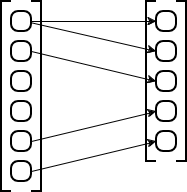
\includegraphics[width=0.3\textwidth]{warp_precompute}
\caption{Index Array Mapping}
\label{fig:warppre}
\end{figure}

\section{Data Normalization}
\label{app:imp-norm}

As noted in \reflink{sec:norm}{subsection}, determining which voxel-based radiomic features require log scaling for distribution normalization is handled programmatically. This process involves loading each feature across all records and analyzing their distribution both before and after log scaling.\par
Initially, the feature is min-max scaled, and the distribution of non-zero voxels is calculated using $100$ bins (bin size $0.01$). Excluding zero values masks the background, which would distort the distribution. However, this exclusion should have been done with the provided brain masks, which would have been more appropriate since zeros could naturally occur in the features. This oversight, while suboptimal, does not significantly affect the results, as non-background zero counts are negligible. And the only consequence is a potential false negative artifacts (failing to apply normalization where needed), which does not degrade the raw data by inappropriately normalizing features.\par
Next, the logarithm is applied to the feature prior to min-max scaling, and the distribution is recalculated using the same $100$ bin approach. The criteria for selecting normalized features are based on observing an increased standard deviation and a reduced count of voxels in the largest bin after normalization. This ensures that features with 'flattened' and 'stretched' distributions are selected for normalization.








\titlespacing*{\chapter}{0pt}{-70pt}{30pt}
\chapter{Additional Figures}
\begin{figure}[H]
\centering
\includegraphics[width=0.9\textwidth]{rad_gldm_small_scale_16}
\includegraphics[width=0.9\textwidth]{rad_gldm_small_scale_32}
\includegraphics[width=0.9\textwidth]{rad_gldm_small_norm_16}
\caption{Slice: GLDM Small Dependence High Gray Level Emphasis}
\label{fig:gls}
\end{figure}

\begin{figure}[H]
\centering
\includegraphics[width=0.9\textwidth]{rad_ngtdm_busyness_scale_16}
\includegraphics[width=0.9\textwidth]{rad_ngtdm_busyness_scale_32}
\includegraphics[width=0.9\textwidth]{rad_ngtdm_busyness_norm_16}
\caption{Slice: NGTDM Busyness}
\label{fig:ngb}
\end{figure}

\begin{figure}[H]
\centering
\includegraphics[width=0.7\textwidth]{subcortical_curve}
\caption{Training Curve: Subcortical}
\label{fig:curve-sub}
\end{figure}

\begin{figure}[H]
\centering
\includegraphics[width=0.9\textwidth]{subcortical_train_o}
\includegraphics[width=0.9\textwidth]{subcortical_train_p}
\caption{Train Predictions: Subcortical}
\label{fig:pred-tra-sub}
\end{figure}

\begin{figure}[H]
\centering
\includegraphics[width=0.9\textwidth]{subcortical_val_o}
\includegraphics[width=0.9\textwidth]{subcortical_val_p}
\caption{Validation Predictions: Subcortical}
\label{fig:pred-val-sub}
\end{figure}

\begin{figure}[H]
\centering
\includegraphics[width=0.9\textwidth]{subcortical_test_o}
\includegraphics[width=0.9\textwidth]{subcortical_test_p}
\caption{Test Predictions: Subcortical}
\label{fig:pred-tes-sub}
\end{figure}





\titlespacing*{\chapter}{0pt}{-10pt}{30pt}
\chapter{Additional Tables}
\bgroup
\setlength\LTleft{-1cm}
\setlength\LTright{-1cm}
\begin{longtable}[H]{|l|l|l|}
\nobreakhline
\textbf{First Order} & \textbf{\ac{GLCM}} & \textbf{\ac{GLSZM}} \\ \nobreakhline
Energy & Autocorrelation & SmallAreaEmphasis \\ \nobreakhline
TotalEnergy & JointAverage & LargeAreaEmphasis \\ \nobreakhline
Entropy & ClusterProminence & GrayLevelNonUniformity \\ \nobreakhline
Minimum & ClusterShade & GrayLevelNonUniformityNormalized \\ \nobreakhline
10Percentile & ClusterTendency & SizeZoneNonUniformity \\ \nobreakhline
90Percentile & Contrast & SizeZoneNonUniformityNormalized \\ \nobreakhline
Maximum & Correlation & ZonePercentage \\ \nobreakhline
Mean & DifferenceAverage & GrayLevelVariance \\ \nobreakhline
Median & DifferenceEntropy & ZoneVariance \\ \nobreakhline
InterquartileRange & DifferenceVariance & ZoneEntropy \\ \nobreakhline
Range & JointEnergy & LowGrayLevelZoneEmphasis \\ \nobreakhline
MeanAbsoluteDeviation & JointEntropy & HighGrayLevelZoneEmphasis \\ \nobreakhline
RobustMeanAbsoluteDeviation & Imc1 & SmallAreaLowGrayLevelEmphasis \\ \nobreakhline
RootMeanSquared & Imc2 & SmallAreaHighGrayLevelEmphasis \\ \hline
Skewness & Idm & LargeAreaLowGrayLevelEmphasis \\ \nobreakhline
Kurtosis & MCC & LargeAreaHighGrayLevelEmphasis \\ \nobreakhline
Variance & Idmn &  \\ \nobreakhline
Uniformity & Id &  \\ \nobreakhline
 & Idn &  \\ \nobreakhline
 & InverseVariance &  \\ \nobreakhline
 & MaximumProbability &  \\ \nobreakhline
 & SumEntropy &  \\ \nobreakhline
 & SumSquares &  \\ \hline \hline
\textbf{\ac{GLRLM}} & \textbf{\ac{NGTDM}} & \textbf{\ac{GLDM}} \\ \nobreakhline
ShortRunEmphasis & Coarseness & SmallDependenceEmphasis \\ \nobreakhline
LongRunEmphasis & Contrast & LargeDependenceEmphasis \\ \nobreakhline
GrayLevelNonUniformity & Busyness & GrayLevelNonUniformity \\ \nobreakhline
GrayLevelNonUniformityNormalized & Complexity & DependenceNonUniformity \\ \nobreakhline
RunLengthNonUniformity & Strength & DependenceNonUniformityNormalized \\ \nobreakhline
RunLengthNonUniformityNormalized &  & GrayLevelVariance \\ \nobreakhline
RunPercentage &  & DependenceVariance \\ \nobreakhline
GrayLevelVariance &  & DependenceEntropy \\ \nobreakhline
RunVariance &  & LowGrayLevelEmphasis \\ \nobreakhline
RunEntropy &  & HighGrayLevelEmphasis \\ \nobreakhline
LowGrayLevelRunEmphasis &  & SmallDependenceLowGrayLevelEmphasis \\ \nobreakhline
HighGrayLevelRunEmphasis &  & SmallDependenceHighGrayLevelEmphasis \\ \nobreakhline
ShortRunLowGrayLevelEmphasis &  & LargeDependenceLowGrayLevelEmphasis \\ \nobreakhline
ShortRunHighGrayLevelEmphasis &  & LargeDependenceHighGrayLevelEmphasis \\ \nobreakhline
LongRunLowGrayLevelEmphasis &  &  \\ \nobreakhline
LongRunHighGrayLevelEmphasis &  &  \\ \nobreakhline
\caption{Voxel Based Radiomic Features}
\label{tab:radf1}
\end{longtable}
\egroup

\begin{table}[H]
\centering
\begin{tabular}{|l|}
\hline
\textbf{3D Shape} \\ \hline
MeshVolume \\ \hline
VoxelVolume \\ \hline
SurfaceArea \\ \hline
SurfaceVolumeRatio \\ \hline
Sphericity \\ \hline
Maximum3DDiameter \\ \hline
Maximum2DDiameterSlice \\ \hline
Maximum2DDiameterColumn \\ \hline
Maximum2DDiameterRow \\ \hline
MajorAxisLength \\ \hline
MinorAxisLength \\ \hline
LeastAxisLength \\ \hline
Elongation \\ \hline
Flatness \\ \hline
\end{tabular}
\caption{Shape Based Radiomic Features}
\label{tab:radf2}
\end{table}

\pagebreak
\afterpage{
  \KOMAoptions{paper=landscape,pagesize}
  \thispagestyle{empty}
  \vspace*{-2.1cm}
  \bgroup
  \setlength\LTleft{-0.5cm}
  \setlength\LTright{-0.5cm}
  \begin{longtable}[H]{|p{0.6cm}|p{10.3cm}|p{1.1cm}|p{1.1cm}|p{1.1cm}|p{1.1cm}|p{1.1cm}|p{1.1cm}|p{1.1cm}|p{1.1cm}|p{1.1cm}|r|}
  \hline
  \textbf{ID} & \textbf{Experiment} & \multicolumn{3}{c|}{\textbf{Raw}} & \multicolumn{3}{c|}{\textbf{Native}} & \multicolumn{3}{c|}{\textbf{Normalized}} & \textbf{Input} \\ \cline{3-11}
   &  & \textbf{Train} & \textbf{Val} & \textbf{Test} & \textbf{Train} & \textbf{Val} & \textbf{Test} & \textbf{Train} & \textbf{Val} & \textbf{Test} & \textbf{Layer} \\ \hline
1. & \textbf{single\_vox} & $58.3$ & $64.9$ & $59.7$ & $60.0$ & $64.3$ & $61.1$ & $60.9$ & $65.0$ & $62.5$ & $92$ \\ \hline
2. & \textbf{single\_vox-single\_targets} & $66.1$ & $67.1$ & $61.4$ & $65.2$ & $69.0$ & $64.6$ & $65.7$ & $69.1$ & $66.1$ & $1576$ \\ \hline
3. & \textbf{single\_vox-single\_roi} & $62.1$ & $65.4$ & $58.2$ & $62.5$ & $67.2$ & $61.5$ & $63.0$ & $67.3$ & $63.5$ & $304$ \\ \hline
4. & \textbf{single\_vox-single\_brain} & $66.1$ & $66.9$ & $66.3$ & $65.9$ & $69.4$ & $66.5$ & $66.4$ & $69.3$ & $67.7$ & $198$ \\ \hline
5. & \textbf{single\_vox-many\_brain} & $64.8$ & $66.7$ & $63.7$ & $64.4$ & $68.4$ & $64.1$ & $64.8$ & $68.4$ & $65.7$ & $474$ \\ \hline
6. & \textbf{many\_vox-single\_brain} & $78.6$ & $77.7$ & $77.4$ & $78.5$ & $79.4$ & $77.5$ & $78.7$ & $79.0$ & $78.4$ & $934$ \\ \hline
7. & \textbf{many\_vox-CLR} & $80.0$ & $79.3$ & $79.6$ & \textbf{80.1} & \textbf{81.1} & \textbf{79.5} & \textbf{80.4} & \textbf{80.9} & \textbf{80.0} & $828$ \\ \hline
8. & \textbf{many\_vox-CL} & $79.6$ & $79.4$ & $76.6$ & $79.6$ & $80.8$ & $76.9$ & $80.7$ & $81.1$ & $78.6$ & $828$ \\ \hline
9. & \textbf{many\_vox-CR} & $81.9$ & $82.2$ & $79.8$ & $82.3$ & $83.5$ & $79.9$ & $81.9$ & $83.2$ & $79.3$ & $828$ \\ \hline
10. & \textbf{many\_vox-HLR} & $78.2$ & $79.0$ & $74.6$ & $77.9$ & $78.6$ & $77.1$ & $78.2$ & $78.7$ & $78.6$ & $828$ \\ \hline
11. & \textbf{many\_vox-HL} & $76.7$ & $73.9$ & $73.2$ & $76.1$ & $75.9$ & $74.7$ & $78.2$ & $78.2$ & $78.7$ & $828$ \\ \hline
12. & \textbf{many\_vox-HR} & $79.3$ & $80.9$ & $73.7$ & $79.4$ & $80.3$ & $76.6$ & $78.2$ & $78.9$ & $76.6$ & $828$ \\ \hline
13. & \textbf{many\_vox-HLR-clinical\_CAP} & $80.7$ & $76.4$ & $81.0$ & $80.3$ & $77.1$ & $81.1$ & $80.7$ & $78.3$ & $79.4$ & $829$ \\ \hline
14. & \textbf{many\_vox-HLR-clinical\_UHDRS} & $76.8$ & $73.3$ & $76.6$ & $76.5$ & $74.3$ & $77.5$ & $76.9$ & $75.6$ & $75.7$ & $832$ \\ \hline
15. & \textbf{many\_vox-HLR-clinical\_all} & $75.0$ & $66.7$ & $72.9$ & $74.1$ & $72.1$ & $75.3$ & $74.5$ & $73.4$ & $73.4$ & $919$ \\ \hline
16. & \textbf{many\_vox-CHLR} & $79.3$ & $80.5$ & $78.5$ & $79.3$ & $81.2$ & $80.0$ & $79.5$ & $81.2$ & $81.0$ & $828$ \\ \hline
17. & \textbf{many\_vox-CHL} & $77.5$ & $77.4$ & $74.3$ & $77.5$ & $79.1$ & $76.6$ & $79.0$ & $80.4$ & $79.3$ & $828$ \\ \hline
18. & \textbf{many\_vox-CHR} & $81.2$ & $82.7$ & $79.9$ & $81.3$ & $83.3$ & $81.1$ & $80.6$ & $82.6$ & $80.7$ & $828$ \\ \hline
19. & \textbf{many\_vox-CLR\_coords} & $79.5$ & $79.3$ & $79.0$ & $79.7$ & $81.0$ & $79.0$ & $80.0$ & $80.8$ & $79.6$ & $831$ \\ \hline
20. & \textbf{many\_vox-CLR\_scale} & $79.6$ & $79.0$ & $78.9$ & $79.8$ & $80.6$ & $78.8$ & $80.0$ & $80.3$ & $79.3$ & $828$ \\ \hline
21. & \textbf{many\_vox-CLR\_b50} & $80.1$ & $79.5$ & $77.8$ & $80.2$ & $80.2$ & $77.9$ & $80.5$ & $80.1$ & $78.4$ & $828$ \\ \hline
22. & \textbf{many\_vox-CLR-balance\_025} & $51.6$ & $68.5$ & $73.9$ & $80.3$ & $81.0$ & $79.1$ & $80.5$ & $80.7$ & $79.6$ & $828$ \\ \hline
23. & \textbf{many\_vox-CLR-balance\_050} & $45.8$ & $66.6$ & $72.7$ & $79.7$ & $80.9$ & $79.1$ & $79.9$ & $80.7$ & $79.6$ & $828$ \\ \hline
24. & \textbf{many\_vox-CLR-balance\_075} & $41.8$ & $63.5$ & $70.6$ & $80.6$ & $81.0$ & $79.0$ & $80.8$ & $80.8$ & $79.6$ & $828$ \\ \hline
25. & \textbf{many\_vox-CLR-balance\_100} & $41.1$ & $63.1$ & $67.9$ & $79.1$ & $80.1$ & $78.0$ & $79.3$ & $79.8$ & $78.8$ & $828$ \\ \hline
27. & \textbf{many\_vox-CLR-reinclude} & $80.5$ & $79.1$ & $79.3$ & $80.7$ & $81.1$ & $79.3$ & $81.1$ & $80.9$ & $79.7$ & $828$ \\ \hline
  \caption{Hyperparameter Tuning: Diffusion Fractional Anisotropy - Native T1}
  \label{fig:fa-nat-t1}
  \end{longtable}
  \egroup
  \clearpage
  \KOMAoptions{paper=portrait,pagesize}
}
\pagebreak
\afterpage{
  \KOMAoptions{paper=landscape,pagesize}
  \thispagestyle{empty}
  \vspace*{-2.1cm}
  \bgroup
  \setlength\LTleft{-0.5cm}
  \setlength\LTright{-0.5cm}
  \begin{longtable}[H]{|p{0.6cm}|p{10.3cm}|p{1.1cm}|p{1.1cm}|p{1.1cm}|p{1.1cm}|p{1.1cm}|p{1.1cm}|p{1.1cm}|p{1.1cm}|p{1.1cm}|r|}
  \hline
  \textbf{ID} & \textbf{Experiment} & \multicolumn{3}{c|}{\textbf{Raw}} & \multicolumn{3}{c|}{\textbf{Native}} & \multicolumn{3}{c|}{\textbf{Normalized}} & \textbf{Input} \\ \cline{3-11}
   &  & \textbf{Train} & \textbf{Val} & \textbf{Test} & \textbf{Train} & \textbf{Val} & \textbf{Test} & \textbf{Train} & \textbf{Val} & \textbf{Test} & \textbf{Layer} \\ \hline
1. & \textbf{single\_vox} & $63.1$ & $70.1$ & $62.2$ & $66.2$ & $69.8$ & $68.2$ & $66.6$ & $69.9$ & $69.2$ & $92$ \\ \hline
2. & \textbf{single\_vox-single\_targets} & $70.6$ & $71.2$ & $64.3$ & $69.4$ & $71.3$ & $66.5$ & $69.5$ & $71.1$ & $67.6$ & $1576$ \\ \hline
3. & \textbf{single\_vox-single\_roi} & $67.1$ & $69.0$ & $65.5$ & $66.2$ & $69.8$ & $66.7$ & $66.5$ & $69.8$ & $67.6$ & $304$ \\ \hline
4. & \textbf{single\_vox-single\_brain} & $67.1$ & $70.6$ & $64.6$ & $67.0$ & $70.8$ & $67.0$ & $67.3$ & $70.7$ & $68.0$ & $198$ \\ \hline
5. & \textbf{single\_vox-many\_brain} & $67.6$ & $70.3$ & $66.5$ & $67.3$ & $70.8$ & $67.5$ & $67.5$ & $70.8$ & $68.4$ & $474$ \\ \hline
6. & \textbf{many\_vox-single\_brain} & $81.0$ & $80.7$ & $78.8$ & $80.9$ & $80.5$ & $79.4$ & $81.1$ & $80.5$ & $79.9$ & $934$ \\ \hline
7. & \textbf{many\_vox-CLR} & $80.1$ & $79.7$ & $76.3$ & $80.5$ & $79.8$ & $77.8$ & $80.8$ & $79.9$ & $78.7$ & $828$ \\ \hline
8. & \textbf{many\_vox-CL} & $77.2$ & $78.1$ & $72.5$ & $77.9$ & $78.5$ & $77.2$ & $79.1$ & $79.5$ & $79.7$ & $828$ \\ \hline
9. & \textbf{many\_vox-CR} & $79.9$ & $80.0$ & $77.2$ & $80.6$ & $79.3$ & $78.3$ & $80.1$ & $79.0$ & $78.3$ & $828$ \\ \hline
10. & \textbf{many\_vox-HLR} & $79.9$ & $74.3$ & $78.6$ & $79.5$ & $76.2$ & $78.5$ & $79.7$ & $76.1$ & $80.5$ & $828$ \\ \hline
11. & \textbf{many\_vox-HL} & $72.1$ & $58.9$ & $71.4$ & $72.6$ & $69.4$ & $71.5$ & $75.3$ & $72.2$ & $76.3$ & $828$ \\ \hline
12. & \textbf{many\_vox-HR} & $75.6$ & $75.7$ & $74.9$ & $75.7$ & $76.2$ & $75.0$ & $74.2$ & $74.7$ & $75.0$ & $828$ \\ \hline
13. & \textbf{many\_vox-HLR-clinical\_CAP} & $75.1$ & $75.2$ & $72.5$ & $75.4$ & $76.0$ & $73.4$ & $75.8$ & $76.8$ & $72.6$ & $829$ \\ \hline
14. & \textbf{many\_vox-HLR-clinical\_UHDRS} & $80.2$ & $77.4$ & $78.2$ & $79.8$ & $77.7$ & $78.2$ & $80.2$ & $78.5$ & $77.2$ & $832$ \\ \hline
15. & \textbf{many\_vox-HLR-clinical\_all} & $76.2$ & $70.5$ & $71.5$ & $75.3$ & $73.5$ & $72.9$ & $75.7$ & $74.7$ & $71.8$ & $919$ \\ \hline
16. & \textbf{many\_vox-CHLR} & $75.8$ & $74.4$ & $72.6$ & $76.4$ & $75.8$ & $76.4$ & $76.6$ & $75.8$ & $77.7$ & $828$ \\ \hline
17. & \textbf{many\_vox-CHL} & $77.4$ & $72.1$ & $72.6$ & $77.6$ & $74.2$ & $77.3$ & $79.2$ & $75.8$ & $80.3$ & $828$ \\ \hline
18. & \textbf{many\_vox-CHR} & $75.5$ & $75.6$ & $73.1$ & $76.2$ & $76.0$ & $75.3$ & $75.1$ & $74.8$ & $75.4$ & $828$ \\ \hline
19. & \textbf{many\_vox-CLR\_coords} & $80.2$ & $80.2$ & $77.4$ & $80.6$ & $80.2$ & $78.4$ & $80.9$ & $80.4$ & $79.3$ & $831$ \\ \hline
20. & \textbf{many\_vox-CLR\_scale} & $80.8$ & $80.3$ & $75.9$ & $81.2$ & $80.1$ & $77.5$ & $81.5$ & $80.2$ & $78.4$ & $828$ \\ \hline
21. & \textbf{many\_vox-CLR\_b50} & $79.8$ & $80.6$ & $74.9$ & $80.3$ & $80.2$ & $77.2$ & $80.6$ & $80.1$ & $78.3$ & $828$ \\ \hline
22. & \textbf{many\_vox-CLR-balance\_025} & $57.0$ & $68.0$ & $74.6$ & $80.8$ & $80.0$ & $78.2$ & $81.1$ & $80.2$ & $79.2$ & $828$ \\ \hline
23. & \textbf{many\_vox-CLR-balance\_050} & $51.8$ & $64.9$ & $72.6$ & $81.0$ & $80.2$ & $78.3$ & $81.2$ & $80.3$ & $79.2$ & $828$ \\ \hline
24. & \textbf{many\_vox-CLR-balance\_075} & $47.3$ & $62.6$ & $71.0$ & $80.9$ & $79.8$ & $77.4$ & $81.2$ & $80.0$ & $78.4$ & $828$ \\ \hline
25. & \textbf{many\_vox-CLR-balance\_100} & $43.8$ & $62.5$ & $70.4$ & $79.6$ & $79.3$ & $77.8$ & $79.9$ & $79.5$ & $78.8$ & $828$ \\ \hline
28. & \textbf{many\_vox-single\_brain-coords} & $81.4$ & $81.0$ & $79.0$ & \textbf{81.3} & \textbf{80.8} & \textbf{79.7} & \textbf{81.6} & \textbf{80.8} & \textbf{80.3} & $937$ \\ \hline
  \caption{Hyperparameter Tuning: Diffusion Fractional Anisotropy - Native T1/T2}
  \label{fig:fa-nat-t1t2}
  \end{longtable}
  \egroup
  \clearpage
  \KOMAoptions{paper=portrait,pagesize}
}
\pagebreak
\afterpage{
  \KOMAoptions{paper=landscape,pagesize}
  \thispagestyle{empty}
  \vspace*{-2.1cm}
  \bgroup
  \setlength\LTleft{-0.5cm}
  \setlength\LTright{-0.5cm}
  \begin{longtable}[H]{|p{0.6cm}|p{10.3cm}|p{1.1cm}|p{1.1cm}|p{1.1cm}|p{1.1cm}|p{1.1cm}|p{1.1cm}|p{1.1cm}|p{1.1cm}|p{1.1cm}|r|}
  \hline
  \textbf{ID} & \textbf{Experiment} & \multicolumn{3}{c|}{\textbf{Raw}} & \multicolumn{3}{c|}{\textbf{Native}} & \multicolumn{3}{c|}{\textbf{Normalized}} & \textbf{Input} \\ \cline{3-11}
   &  & \textbf{Train} & \textbf{Val} & \textbf{Test} & \textbf{Train} & \textbf{Val} & \textbf{Test} & \textbf{Train} & \textbf{Val} & \textbf{Test} & \textbf{Layer} \\ \hline
1. & \textbf{single\_vox} & $52.5$ & $58.9$ & $53.4$ & $54.2$ & $60.3$ & $54.9$ & $54.4$ & $59.3$ & $54.2$ & $92$ \\ \hline
2. & \textbf{single\_vox-single\_targets} & $60.1$ & $56.7$ & $58.8$ & $60.3$ & $64.0$ & $61.4$ & $60.5$ & $63.8$ & $60.8$ & $1380$ \\ \hline
3. & \textbf{single\_vox-single\_roi} & $65.2$ & $67.1$ & $63.3$ & $64.0$ & $68.9$ & $65.6$ & $64.3$ & $68.6$ & $65.2$ & $276$ \\ \hline
4. & \textbf{single\_vox-single\_brain} & $65.3$ & $66.1$ & $65.8$ & $64.5$ & $68.9$ & $66.0$ & $64.8$ & $68.6$ & $65.9$ & $184$ \\ \hline
5. & \textbf{single\_vox-many\_brain} & $60.6$ & $62.7$ & $61.8$ & $61.5$ & $66.1$ & $62.5$ & $61.8$ & $65.8$ & $62.0$ & $460$ \\ \hline
6. & \textbf{many\_vox-single\_brain} & $81.9$ & $82.3$ & $80.8$ & $81.4$ & $83.2$ & $81.0$ & $81.6$ & $83.4$ & $81.5$ & $920$ \\ \hline
7. & \textbf{many\_vox-CLR} & $82.3$ & $82.1$ & $80.8$ & $82.0$ & $83.4$ & $81.3$ & $82.3$ & $83.7$ & $81.7$ & $828$ \\ \hline
8. & \textbf{many\_vox-CL} & $81.8$ & $81.3$ & $79.8$ & $82.5$ & $83.9$ & $82.9$ & $81.8$ & $83.5$ & $81.6$ & $828$ \\ \hline
9. & \textbf{many\_vox-CR} & $83.6$ & $83.2$ & $82.8$ & $82.8$ & $83.5$ & $81.5$ & $83.9$ & $84.2$ & $82.9$ & $828$ \\ \hline
10. & \textbf{many\_vox-HLR} & $76.4$ & $72.9$ & $64.0$ & $76.4$ & $75.8$ & $70.0$ & $75.4$ & $74.3$ & $68.5$ & $828$ \\ \hline
11. & \textbf{many\_vox-HL} & $77.0$ & $71.8$ & $66.3$ & $79.2$ & $77.9$ & $73.2$ & $76.7$ & $74.4$ & $69.3$ & $828$ \\ \hline
12. & \textbf{many\_vox-HR} & $75.0$ & $73.5$ & $60.9$ & $73.0$ & $73.5$ & $66.6$ & $74.1$ & $74.5$ & $67.9$ & $828$ \\ \hline
13. & \textbf{many\_vox-HLR-clinical\_CAP} & $77.2$ & $77.5$ & $66.1$ & $77.6$ & $78.0$ & $64.1$ & $76.5$ & $76.3$ & $64.0$ & $829$ \\ \hline
14. & \textbf{many\_vox-HLR-clinical\_UHDRS} & $75.7$ & $75.6$ & $64.6$ & $76.2$ & $76.6$ & $62.8$ & $75.1$ & $74.8$ & $62.6$ & $832$ \\ \hline
15. & \textbf{many\_vox-HLR-clinical\_all} & $71.8$ & $69.7$ & $65.3$ & $72.4$ & $72.3$ & $65.7$ & $71.0$ & $70.7$ & $64.8$ & $919$ \\ \hline
16. & \textbf{many\_vox-CHLR} & $80.8$ & $80.1$ & $75.7$ & $80.6$ & $81.5$ & $79.1$ & $80.3$ & $81.1$ & $78.7$ & $828$ \\ \hline
17. & \textbf{many\_vox-CHL} & $79.9$ & $77.7$ & $73.9$ & $81.2$ & $81.9$ & $79.6$ & $79.6$ & $80.0$ & $77.5$ & $828$ \\ \hline
18. & \textbf{many\_vox-CHR} & $81.5$ & $82.0$ & $77.5$ & $80.5$ & $81.5$ & $79.0$ & $81.3$ & $82.2$ & $79.9$ & $828$ \\ \hline
19. & \textbf{many\_vox-CLR\_coords} & $81.7$ & $81.6$ & $81.0$ & $81.5$ & $83.3$ & $81.4$ & $81.7$ & $83.5$ & $81.7$ & $831$ \\ \hline
20. & \textbf{many\_vox-CLR\_scale} & $84.4$ & $82.9$ & $82.0$ & $84.1$ & $84.4$ & $82.4$ & $84.3$ & $84.8$ & $82.6$ & $828$ \\ \hline
22. & \textbf{many\_vox-CLR-balance\_025} & $58.2$ & $80.7$ & $85.6$ & $82.7$ & $83.5$ & $81.7$ & $82.9$ & $83.8$ & $82.0$ & $828$ \\ \hline
23. & \textbf{many\_vox-CLR-balance\_050} & $55.3$ & $79.8$ & $86.5$ & $84.0$ & $84.2$ & $82.4$ & $84.3$ & $84.6$ & $82.7$ & $828$ \\ \hline
24. & \textbf{many\_vox-CLR-balance\_075} & $51.2$ & $79.2$ & $86.0$ & $83.4$ & $84.0$ & $81.9$ & $83.7$ & $84.4$ & $82.1$ & $828$ \\ \hline
25. & \textbf{many\_vox-CLR-balance\_100} & $46.2$ & $78.2$ & $84.8$ & $81.9$ & $83.1$ & $81.2$ & $82.1$ & $83.4$ & $81.5$ & $828$ \\ \hline
27. & \textbf{many\_vox-CLR-reinclude} & $84.6$ & $83.3$ & $82.3$ & \textbf{84.4} & \textbf{84.6} & \textbf{82.8} & \textbf{84.6} & \textbf{84.9} & \textbf{82.9} & $828$ \\ \hline
28. & \textbf{many\_vox-scale-bal50-reinclude} & $96.3$ & $83.8$ & $81.7$ & $76.8$ & $77.1$ & $77.3$ & $76.8$ & $76.6$ & $76.9$ & $828$ \\ \hline
29. & \textbf{many\_vox-bal50-reinclude} & $96.2$ & $83.1$ & $83.9$ & $76.9$ & $77.1$ & $77.7$ & $76.9$ & $76.6$ & $77.3$ & $828$ \\ \hline
  \caption{Hyperparameter Tuning: Diffusion Fractional Anisotropy - Normalized T1}
  \label{fig:fa-norm-t1}
  \end{longtable}
  \egroup
  \clearpage
  \KOMAoptions{paper=portrait,pagesize}
}
\pagebreak
\afterpage{
  \KOMAoptions{paper=landscape,pagesize}
  \thispagestyle{empty}
  \vspace*{-2.1cm}
  \bgroup
  \setlength\LTleft{-0.5cm}
  \setlength\LTright{-0.5cm}
  \begin{longtable}[H]{|p{0.6cm}|p{10.3cm}|p{1.1cm}|p{1.1cm}|p{1.1cm}|p{1.1cm}|p{1.1cm}|p{1.1cm}|p{1.1cm}|p{1.1cm}|p{1.1cm}|r|}
  \hline
  \textbf{ID} & \textbf{Experiment} & \multicolumn{3}{c|}{\textbf{Raw}} & \multicolumn{3}{c|}{\textbf{Native}} & \multicolumn{3}{c|}{\textbf{Normalized}} & \textbf{Input} \\ \cline{3-11}
   &  & \textbf{Train} & \textbf{Val} & \textbf{Test} & \textbf{Train} & \textbf{Val} & \textbf{Test} & \textbf{Train} & \textbf{Val} & \textbf{Test} & \textbf{Layer} \\ \hline
1. & \textbf{single\_vox} & $58.7$ & $66.4$ & $59.8$ & $61.4$ & $66.7$ & $65.0$ & $61.8$ & $66.2$ & $65.1$ & $92$ \\ \hline
2. & \textbf{single\_vox-single\_targets} & $59.8$ & $58.0$ & $58.8$ & $58.8$ & $63.9$ & $61.5$ & $59.0$ & $63.8$ & $61.4$ & $1380$ \\ \hline
3. & \textbf{single\_vox-single\_roi} & $64.3$ & $63.0$ & $66.7$ & $63.0$ & $65.8$ & $66.1$ & $63.3$ & $66.0$ & $66.2$ & $276$ \\ \hline
4. & \textbf{single\_vox-single\_brain} & $66.6$ & $68.8$ & $67.1$ & $65.8$ & $69.1$ & $67.4$ & $66.1$ & $68.9$ & $67.8$ & $184$ \\ \hline
5. & \textbf{single\_vox-many\_brain} & $67.3$ & $68.8$ & $66.9$ & $66.3$ & $69.0$ & $67.2$ & $66.5$ & $68.9$ & $67.6$ & $460$ \\ \hline
6. & \textbf{many\_vox-single\_brain} & $83.4$ & $82.3$ & $82.2$ & \textbf{83.1} & \textbf{82.3} & \textbf{82.7} & \textbf{83.2} & \textbf{82.8} & \textbf{82.7} & $920$ \\ \hline
7. & \textbf{many\_vox-CLR} & $80.7$ & $80.9$ & $79.2$ & $80.9$ & $80.3$ & $81.1$ & $80.9$ & $80.7$ & $81.0$ & $828$ \\ \hline
8. & \textbf{many\_vox-CL} & $79.1$ & $79.8$ & $73.8$ & $80.4$ & $80.3$ & $81.0$ & $79.5$ & $79.5$ & $79.1$ & $828$ \\ \hline
9. & \textbf{many\_vox-CR} & $81.9$ & $81.8$ & $81.9$ & $81.4$ & $80.6$ & $80.8$ & $82.0$ & $81.3$ & $81.8$ & $828$ \\ \hline
10. & \textbf{many\_vox-HLR} & $73.9$ & $62.3$ & $66.0$ & $74.5$ & $69.4$ & $68.5$ & $73.6$ & $66.6$ & $67.2$ & $828$ \\ \hline
11. & \textbf{many\_vox-HL} & $78.1$ & $58.6$ & $66.3$ & $79.9$ & $70.1$ & $72.1$ & $77.7$ & $65.1$ & $67.3$ & $828$ \\ \hline
12. & \textbf{many\_vox-HR} & $74.0$ & $66.5$ & $68.0$ & $72.5$ & $69.0$ & $66.0$ & $73.7$ & $68.2$ & $68.9$ & $828$ \\ \hline
13. & \textbf{many\_vox-HLR-clinical\_CAP} & $78.0$ & $72.9$ & $69.8$ & $78.6$ & $74.2$ & $70.2$ & $77.7$ & $73.8$ & $68.5$ & $829$ \\ \hline
14. & \textbf{many\_vox-HLR-clinical\_UHDRS} & $80.3$ & $77.2$ & $71.2$ & $80.6$ & $77.6$ & $71.8$ & $79.7$ & $77.1$ & $70.0$ & $832$ \\ \hline
15. & \textbf{many\_vox-HLR-clinical\_all} & $69.6$ & $69.0$ & $61.2$ & $70.1$ & $71.2$ & $62.2$ & $68.7$ & $70.0$ & $59.9$ & $919$ \\ \hline
16. & \textbf{many\_vox-CHLR} & $79.9$ & $73.1$ & $75.5$ & $79.9$ & $75.7$ & $78.0$ & $79.5$ & $74.6$ & $77.3$ & $828$ \\ \hline
17. & \textbf{many\_vox-CHL} & $78.9$ & $70.7$ & $69.7$ & $80.4$ & $75.9$ & $78.1$ & $78.9$ & $73.0$ & $75.2$ & $828$ \\ \hline
18. & \textbf{many\_vox-CHR} & $72.1$ & $73.1$ & $69.5$ & $71.4$ & $72.8$ & $69.5$ & $72.7$ & $73.4$ & $72.0$ & $828$ \\ \hline
19. & \textbf{many\_vox-CLR\_coords} & $83.2$ & $82.6$ & $80.8$ & $83.3$ & $81.6$ & $82.1$ & $83.3$ & $82.2$ & $82.0$ & $831$ \\ \hline
20. & \textbf{many\_vox-CLR\_scale} & $79.9$ & $80.3$ & $79.1$ & $79.9$ & $79.6$ & $80.8$ & $80.0$ & $80.0$ & $80.8$ & $828$ \\ \hline
22. & \textbf{many\_vox-CLR-balance\_025} & $68.0$ & $80.2$ & $87.3$ & $81.2$ & $80.3$ & $81.3$ & $81.2$ & $80.9$ & $81.3$ & $828$ \\ \hline
23. & \textbf{many\_vox-CLR-balance\_050} & $61.6$ & $78.2$ & $87.4$ & $82.0$ & $80.8$ & $81.7$ & $82.1$ & $81.3$ & $81.6$ & $828$ \\ \hline
24. & \textbf{many\_vox-CLR-balance\_075} & $63.0$ & $78.0$ & $86.5$ & $79.7$ & $79.5$ & $80.5$ & $79.8$ & $79.9$ & $80.6$ & $828$ \\ \hline
25. & \textbf{many\_vox-CLR-balance\_100} & $59.3$ & $77.4$ & $88.9$ & $83.4$ & $81.4$ & $82.0$ & $83.4$ & $82.0$ & $81.8$ & $828$ \\ \hline
28. & \textbf{many\_vox-brain-coords-bal50} & $96.5$ & $82.4$ & $83.6$ & $77.6$ & $79.9$ & $77.1$ & $77.3$ & $80.1$ & $76.7$ & $923$ \\ \hline
29. & \textbf{many\_vox-brain-coords} & $83.0$ & $82.5$ & $81.8$ & $82.7$ & $82.4$ & $82.4$ & $82.7$ & $82.9$ & $82.3$ & $923$ \\ \hline
  \caption{Hyperparameter Tuning: Diffusion Fractional Anisotropy - Normalized T1/T2}
  \label{fig:fa-norm-t1t2}
  \end{longtable}
  \egroup
  \clearpage
  \KOMAoptions{paper=portrait,pagesize}
}
\pagebreak
\afterpage{
  \KOMAoptions{paper=landscape,pagesize}
  \thispagestyle{empty}
  \vspace*{-2.1cm}
  \bgroup
  \setlength\LTleft{-0.5cm}
  \setlength\LTright{-0.5cm}
  \begin{longtable}[H]{|p{0.6cm}|p{10.3cm}|p{1.1cm}|p{1.1cm}|p{1.1cm}|p{1.1cm}|p{1.1cm}|p{1.1cm}|p{1.1cm}|p{1.1cm}|p{1.1cm}|r|}
  \hline
  \textbf{ID} & \textbf{Experiment} & \multicolumn{3}{c|}{\textbf{Raw}} & \multicolumn{3}{c|}{\textbf{Native}} & \multicolumn{3}{c|}{\textbf{Normalized}} & \textbf{Input} \\ \cline{3-11}
   &  & \textbf{Train} & \textbf{Val} & \textbf{Test} & \textbf{Train} & \textbf{Val} & \textbf{Test} & \textbf{Train} & \textbf{Val} & \textbf{Test} & \textbf{Layer} \\ \hline
27. & \textbf{normalized-t1-many\_vox-CLR-reinclude} & $84.6$ & $83.3$ & $82.3$ & $84.4$ & $84.6$ & $82.8$ & $84.6$ & $84.9$ & $82.9$ & $828$ \\ \hline
1. & \textbf{layers\_2048} & $82.0$ & $82.2$ & $81.1$ & $81.9$ & $83.1$ & $81.3$ & $82.1$ & $83.4$ & $81.7$ & $828$ \\ \hline
2. & \textbf{layers\_1024} & $84.1$ & $83.1$ & $82.1$ & $84.0$ & $84.4$ & $82.5$ & $84.1$ & $84.7$ & $82.8$ & $828$ \\ \hline
3. & \textbf{layers\_512} & $83.2$ & $83.1$ & $81.5$ & $83.1$ & $84.3$ & $82.2$ & $83.2$ & $84.6$ & $82.5$ & $828$ \\ \hline
4. & \textbf{activation\_sigmoid} & $83.4$ & $82.9$ & $81.9$ & $83.3$ & $84.2$ & $82.3$ & $83.5$ & $84.5$ & $82.6$ & $828$ \\ \hline
5. & \textbf{activation\_relu} & $85.7$ & $83.1$ & $82.3$ & $85.5$ & $84.0$ & $82.3$ & $85.7$ & $84.3$ & $82.8$ & $828$ \\ \hline
6. & \textbf{activation\_silu} & $84.7$ & $83.1$ & $82.7$ & $84.6$ & $84.3$ & $82.4$ & $84.7$ & $84.6$ & $83.0$ & $828$ \\ \hline
7. & \textbf{activation\_elu} & $7.2$ & $4.9$ & $7.4$ & $14.3$ & $14.8$ & $14.9$ & $12.5$ & $11.1$ & $13.8$ & $828$ \\ \hline
8. & \textbf{batch\_10e5} & $80.2$ & $81.2$ & $80.1$ & $80.3$ & $82.3$ & $80.2$ & $80.4$ & $82.6$ & $80.7$ & $828$ \\ \hline
9. & \textbf{batch\_10e4} & $83.1$ & $82.7$ & $81.7$ & $83.0$ & $83.8$ & $82.1$ & $83.2$ & $84.2$ & $82.4$ & $828$ \\ \hline
10. & \textbf{batch\_10e3} & $85.5$ & $83.8$ & $82.5$ & \textbf{85.3} & \textbf{84.9} & \textbf{82.8} & \textbf{85.5} & \textbf{85.2} & \textbf{83.1} & $828$ \\ \hline
11. & \textbf{batch\_10e2} & $89.3$ & $83.4$ & $83.6$ & $89.1$ & $84.2$ & $84.2$ & $89.3$ & $84.4$ & $84.3$ & $828$ \\ \hline
12. & \textbf{dropout\_000} & $89.0$ & $84.8$ & $83.0$ & $88.9$ & $86.0$ & $83.6$ & $88.9$ & $86.0$ & $84.0$ & $828$ \\ \hline
13. & \textbf{dropout\_025} & $89.4$ & $84.2$ & $83.9$ & $89.2$ & $85.0$ & $84.0$ & $89.3$ & $85.4$ & $84.4$ & $828$ \\ \hline
14. & \textbf{dropout\_050} & $84.6$ & $83.5$ & $82.2$ & $84.4$ & $84.5$ & $82.6$ & $84.6$ & $84.9$ & $82.9$ & $828$ \\ \hline
15. & \textbf{dropout\_075} & $89.5$ & $84.2$ & $83.0$ & $89.3$ & $85.7$ & $83.3$ & $89.3$ & $85.9$ & $83.7$ & $828$ \\ \hline
16. & \textbf{dropout\_090} & $84.5$ & $83.8$ & $82.4$ & $84.3$ & $84.8$ & $82.7$ & $84.5$ & $85.1$ & $82.9$ & $828$ \\ \hline
17. & \textbf{patience\_4} & $85.3$ & $83.4$ & $82.6$ & $85.2$ & $84.9$ & $82.7$ & $85.3$ & $85.1$ & $83.1$ & $828$ \\ \hline
18. & \textbf{patience\_7} & $86.3$ & $83.1$ & $82.8$ & $86.2$ & $84.9$ & $83.0$ & $86.3$ & $85.1$ & $83.4$ & $828$ \\ \hline
19. & \textbf{patience\_10} & $87.1$ & $84.4$ & $83.3$ & $87.1$ & $85.1$ & $83.8$ & $87.2$ & $85.3$ & $84.2$ & $828$ \\ \hline
20. & \textbf{rate\_10e-4} & $82.9$ & $82.7$ & $80.8$ & $82.8$ & $84.0$ & $81.6$ & $82.9$ & $84.3$ & $81.9$ & $828$ \\ \hline
21. & \textbf{rate\_10e-3} & $85.2$ & $83.9$ & $82.1$ & $85.1$ & $85.0$ & $82.7$ & $85.3$ & $85.2$ & $83.0$ & $828$ \\ \hline
22. & \textbf{rate\_10e-2} & $nan$ & $nan$ & $nan$ & $nan$ & $nan$ & $nan$ & $nan$ & $nan$ & $nan$ & $828$ \\ \hline
  \caption{Architecture Tuning: Diffusion Fractional Anisotropy}
  \label{fig:fa-arch}
  \end{longtable}
  \egroup
  \clearpage
  \KOMAoptions{paper=portrait,pagesize}
}
\pagebreak
\afterpage{
  \KOMAoptions{paper=landscape,pagesize}
  \thispagestyle{empty}
  \vspace*{-2.1cm}
  \bgroup
  \setlength\LTleft{-0.5cm}
  \setlength\LTright{-0.5cm}
  \begin{longtable}[H]{|p{0.6cm}|p{10.3cm}|p{1.1cm}|p{1.1cm}|p{1.1cm}|p{1.1cm}|p{1.1cm}|p{1.1cm}|p{1.1cm}|p{1.1cm}|p{1.1cm}|r|}
  \hline
  \textbf{ID} & \textbf{Experiment} & \multicolumn{3}{c|}{\textbf{Raw}} & \multicolumn{3}{c|}{\textbf{Native}} & \multicolumn{3}{c|}{\textbf{Normalized}} & \textbf{Input} \\ \cline{3-11}
   &  & \textbf{Train} & \textbf{Val} & \textbf{Test} & \textbf{Train} & \textbf{Val} & \textbf{Test} & \textbf{Train} & \textbf{Val} & \textbf{Test} & \textbf{Layer} \\ \hline
1. & \textbf{single\_vox} & $92.6$ & $94.3$ & $94.2$ & $93.1$ & $94.6$ & $94.2$ & $93.9$ & $94.9$ & $95.6$ & $92$ \\ \hline
2. & \textbf{single\_vox-single\_targets} & $93.9$ & $93.6$ & $93.7$ & $93.6$ & $94.4$ & $94.5$ & $94.3$ & $94.6$ & $95.7$ & $1576$ \\ \hline
3. & \textbf{single\_vox-single\_roi} & $93.7$ & $94.9$ & $92.8$ & $93.6$ & $94.6$ & $94.6$ & $94.3$ & $94.8$ & $95.8$ & $304$ \\ \hline
4. & \textbf{single\_vox-single\_brain} & $93.4$ & $94.9$ & $94.9$ & $93.6$ & $94.9$ & $94.8$ & $94.3$ & $95.1$ & $96.0$ & $198$ \\ \hline
5. & \textbf{single\_vox-many\_brain} & $93.2$ & $94.6$ & $94.5$ & $93.4$ & $94.5$ & $94.6$ & $94.1$ & $94.8$ & $95.8$ & $474$ \\ \hline
6. & \textbf{many\_vox-single\_brain} & $94.7$ & $95.8$ & $94.8$ & \textbf{94.7} & \textbf{95.5} & \textbf{95.1} & \textbf{95.4} & \textbf{95.7} & \textbf{96.3} & $934$ \\ \hline
7. & \textbf{many\_vox-CLR} & $94.0$ & $95.3$ & $94.9$ & $94.2$ & $95.2$ & $94.9$ & $94.9$ & $95.4$ & $96.1$ & $828$ \\ \hline
8. & \textbf{many\_vox-CL} & $93.8$ & $94.4$ & $94.6$ & $94.2$ & $94.6$ & $94.7$ & $95.7$ & $95.7$ & $96.6$ & $828$ \\ \hline
9. & \textbf{many\_vox-CR} & $95.0$ & $96.4$ & $94.7$ & $95.2$ & $96.1$ & $94.9$ & $95.0$ & $95.6$ & $95.0$ & $828$ \\ \hline
10. & \textbf{many\_vox-HLR} & $92.4$ & $94.1$ & $93.8$ & $92.4$ & $94.2$ & $93.8$ & $93.3$ & $94.6$ & $94.9$ & $828$ \\ \hline
11. & \textbf{many\_vox-HL} & $91.7$ & $94.2$ & $95.8$ & $91.9$ & $94.7$ & $95.5$ & $94.1$ & $96.1$ & $97.3$ & $828$ \\ \hline
12. & \textbf{many\_vox-HR} & $91.8$ & $93.7$ & $92.2$ & $91.6$ & $95.1$ & $93.4$ & $91.2$ & $94.3$ & $93.6$ & $828$ \\ \hline
13. & \textbf{many\_vox-HLR-clinical\_CAP} & $93.3$ & $89.4$ & $95.2$ & $93.2$ & $90.9$ & $95.1$ & $93.9$ & $92.3$ & $95.3$ & $829$ \\ \hline
14. & \textbf{many\_vox-HLR-clinical\_UHDRS} & $93.6$ & $89.8$ & $94.7$ & $93.4$ & $90.8$ & $94.9$ & $94.1$ & $92.3$ & $95.1$ & $832$ \\ \hline
15. & \textbf{many\_vox-HLR-clinical\_all} & $93.2$ & $88.6$ & $94.3$ & $92.5$ & $90.4$ & $94.6$ & $93.3$ & $92.0$ & $94.9$ & $919$ \\ \hline
16. & \textbf{many\_vox-CHLR} & $93.6$ & $95.1$ & $94.8$ & $93.7$ & $95.4$ & $95.0$ & $94.4$ & $95.7$ & $96.1$ & $828$ \\ \hline
17. & \textbf{many\_vox-CHL} & $93.6$ & $94.3$ & $94.4$ & $94.0$ & $95.3$ & $95.4$ & $95.6$ & $96.4$ & $97.0$ & $828$ \\ \hline
18. & \textbf{many\_vox-CHR} & $93.7$ & $95.5$ & $93.4$ & $93.9$ & $95.9$ & $94.5$ & $93.5$ & $95.3$ & $94.8$ & $828$ \\ \hline
19. & \textbf{many\_vox-CLR\_coords} & $94.5$ & $95.7$ & $95.0$ & $94.6$ & $95.5$ & $95.1$ & $95.3$ & $95.7$ & $96.2$ & $831$ \\ \hline
20. & \textbf{many\_vox-CLR\_scale} & $94.1$ & $95.3$ & $94.9$ & $94.2$ & $95.2$ & $95.0$ & $94.9$ & $95.4$ & $96.1$ & $828$ \\ \hline
21. & \textbf{many\_vox-CLR\_b50} & $93.8$ & $95.1$ & $94.2$ & $93.9$ & $94.8$ & $94.5$ & $94.8$ & $95.1$ & $95.8$ & $828$ \\ \hline
22. & \textbf{many\_vox-CLR-balance\_025} & $95.5$ & $95.9$ & $95.8$ & $94.3$ & $95.3$ & $95.0$ & $95.0$ & $95.5$ & $96.1$ & $828$ \\ \hline
23. & \textbf{many\_vox-CLR-balance\_050} & $95.3$ & $95.8$ & $95.8$ & $94.3$ & $95.2$ & $95.1$ & $95.0$ & $95.4$ & $96.3$ & $828$ \\ \hline
24. & \textbf{many\_vox-CLR-balance\_075} & $95.2$ & $95.3$ & $95.8$ & $94.0$ & $95.0$ & $94.9$ & $94.8$ & $95.2$ & $96.1$ & $828$ \\ \hline
25. & \textbf{many\_vox-CLR-balance\_100} & $95.4$ & $95.7$ & $95.8$ & $94.3$ & $95.2$ & $95.0$ & $95.0$ & $95.4$ & $96.2$ & $828$ \\ \hline
27. & \textbf{many\_vox-CLR-reinclude} & $94.2$ & $95.2$ & $94.9$ & $94.3$ & $95.0$ & $94.9$ & $95.1$ & $95.3$ & $96.2$ & $828$ \\ \hline
28. & \textbf{many\_vox-bal25-coords-brain} & $97.4$ & $96.7$ & $96.7$ & $93.2$ & $94.0$ & $93.6$ & $94.1$ & $94.4$ & $95.1$ & $937$ \\ \hline
29. & \textbf{many\_vox-single\_brain-coords} & $94.0$ & $95.3$ & $94.9$ & $94.2$ & $95.1$ & $95.0$ & $94.9$ & $95.4$ & $96.2$ & $937$ \\ \hline
  \caption{Hyperparameter Tuning: Mean Diffusivity - Native T1}
  \label{fig:md-nat-t1}
  \end{longtable}
  \egroup
  \clearpage
  \KOMAoptions{paper=portrait,pagesize}
}
\pagebreak
\afterpage{
  \KOMAoptions{paper=landscape,pagesize}
  \thispagestyle{empty}
  \vspace*{-2.1cm}
  \bgroup
  \setlength\LTleft{-0.5cm}
  \setlength\LTright{-0.5cm}
  \begin{longtable}[H]{|p{0.6cm}|p{10.3cm}|p{1.1cm}|p{1.1cm}|p{1.1cm}|p{1.1cm}|p{1.1cm}|p{1.1cm}|p{1.1cm}|p{1.1cm}|p{1.1cm}|r|}
  \hline
  \textbf{ID} & \textbf{Experiment} & \multicolumn{3}{c|}{\textbf{Raw}} & \multicolumn{3}{c|}{\textbf{Native}} & \multicolumn{3}{c|}{\textbf{Normalized}} & \textbf{Input} \\ \cline{3-11}
   &  & \textbf{Train} & \textbf{Val} & \textbf{Test} & \textbf{Train} & \textbf{Val} & \textbf{Test} & \textbf{Train} & \textbf{Val} & \textbf{Test} & \textbf{Layer} \\ \hline
1. & \textbf{single\_vox} & $93.0$ & $93.8$ & $94.1$ & $93.6$ & $94.7$ & $94.3$ & $94.3$ & $95.0$ & $95.6$ & $92$ \\ \hline
2. & \textbf{single\_vox-single\_targets} & $94.4$ & $93.9$ & $91.7$ & $93.9$ & $94.7$ & $93.8$ & $94.4$ & $94.9$ & $95.0$ & $1576$ \\ \hline
3. & \textbf{single\_vox-single\_roi} & $94.2$ & $95.2$ & $94.3$ & $93.8$ & $94.8$ & $94.6$ & $94.5$ & $95.1$ & $95.7$ & $304$ \\ \hline
4. & \textbf{single\_vox-single\_brain} & $93.9$ & $95.5$ & $92.2$ & $93.8$ & $94.9$ & $94.0$ & $94.4$ & $95.1$ & $95.2$ & $198$ \\ \hline
5. & \textbf{single\_vox-many\_brain} & $94.0$ & $95.4$ & $91.7$ & $93.7$ & $94.8$ & $93.8$ & $94.3$ & $95.0$ & $95.1$ & $474$ \\ \hline
6. & \textbf{many\_vox-single\_brain} & $94.1$ & $95.2$ & $93.8$ & $94.1$ & $95.0$ & $94.5$ & $94.7$ & $95.3$ & $95.7$ & $934$ \\ \hline
7. & \textbf{many\_vox-CLR} & $94.9$ & $95.1$ & $94.4$ & \textbf{95.1} & \textbf{95.8} & \textbf{94.8} & \textbf{95.6} & \textbf{96.1} & \textbf{95.6} & $828$ \\ \hline
8. & \textbf{many\_vox-CL} & $94.1$ & $93.2$ & $95.5$ & $94.6$ & $95.3$ & $95.4$ & $95.9$ & $96.4$ & $96.9$ & $828$ \\ \hline
9. & \textbf{many\_vox-CR} & $95.0$ & $96.3$ & $91.4$ & $95.3$ & $96.6$ & $92.8$ & $94.9$ & $96.1$ & $92.0$ & $828$ \\ \hline
10. & \textbf{many\_vox-HLR} & $92.2$ & $94.6$ & $95.5$ & $92.6$ & $94.7$ & $95.3$ & $93.3$ & $94.9$ & $96.4$ & $828$ \\ \hline
11. & \textbf{many\_vox-HL} & $92.9$ & $94.0$ & $96.1$ & $93.5$ & $94.5$ & $95.9$ & $95.3$ & $96.0$ & $97.6$ & $828$ \\ \hline
12. & \textbf{many\_vox-HR} & $92.7$ & $94.9$ & $94.6$ & $93.3$ & $95.1$ & $95.5$ & $92.8$ & $94.2$ & $95.4$ & $828$ \\ \hline
13. & \textbf{many\_vox-HLR-clinical\_CAP} & $92.7$ & $90.5$ & $93.3$ & $92.9$ & $91.9$ & $94.2$ & $93.6$ & $93.0$ & $94.3$ & $829$ \\ \hline
14. & \textbf{many\_vox-HLR-clinical\_UHDRS} & $93.0$ & $90.6$ & $93.5$ & $92.8$ & $91.8$ & $94.1$ & $93.5$ & $93.0$ & $94.2$ & $832$ \\ \hline
15. & \textbf{many\_vox-HLR-clinical\_all} & $92.8$ & $88.9$ & $93.9$ & $92.2$ & $90.9$ & $94.3$ & $93.1$ & $92.1$ & $94.5$ & $919$ \\ \hline
16. & \textbf{many\_vox-CHLR} & $93.3$ & $94.7$ & $94.9$ & $93.7$ & $95.3$ & $95.0$ & $94.4$ & $95.6$ & $96.1$ & $828$ \\ \hline
17. & \textbf{many\_vox-CHL} & $93.0$ & $92.8$ & $95.6$ & $93.7$ & $95.0$ & $95.6$ & $95.3$ & $96.3$ & $97.1$ & $828$ \\ \hline
18. & \textbf{many\_vox-CHR} & $93.9$ & $96.2$ & $94.5$ & $94.5$ & $96.4$ & $94.9$ & $94.1$ & $95.8$ & $94.7$ & $828$ \\ \hline
19. & \textbf{many\_vox-CLR\_coords} & $94.8$ & $95.2$ & $94.3$ & $95.0$ & $95.9$ & $94.6$ & $95.5$ & $96.2$ & $95.6$ & $831$ \\ \hline
20. & \textbf{many\_vox-CLR\_scale} & $94.4$ & $94.9$ & $94.3$ & $94.7$ & $95.8$ & $94.5$ & $95.3$ & $96.1$ & $95.4$ & $828$ \\ \hline
21. & \textbf{many\_vox-CLR\_b50} & $94.7$ & $95.1$ & $94.5$ & $94.9$ & $95.8$ & $94.6$ & $95.4$ & $96.1$ & $95.6$ & $828$ \\ \hline
22. & \textbf{many\_vox-CLR-balance\_025} & $96.4$ & $95.4$ & $95.7$ & $94.7$ & $95.8$ & $94.6$ & $95.2$ & $96.1$ & $95.6$ & $828$ \\ \hline
23. & \textbf{many\_vox-CLR-balance\_050} & $96.6$ & $95.5$ & $95.1$ & $94.9$ & $95.8$ & $94.7$ & $95.5$ & $96.1$ & $95.6$ & $828$ \\ \hline
24. & \textbf{many\_vox-CLR-balance\_075} & $96.3$ & $95.2$ & $95.4$ & $94.6$ & $95.7$ & $94.6$ & $95.2$ & $96.0$ & $95.6$ & $828$ \\ \hline
25. & \textbf{many\_vox-CLR-balance\_100} & $96.3$ & $95.3$ & $95.2$ & $94.7$ & $95.7$ & $94.9$ & $95.3$ & $96.0$ & $95.9$ & $828$ \\ \hline
  \caption{Hyperparameter Tuning: Mean Diffusivity - Native T1/T2}
  \label{fig:md-nat-t1t2}
  \end{longtable}
  \egroup
  \clearpage
  \KOMAoptions{paper=portrait,pagesize}
}
\pagebreak
\afterpage{
  \KOMAoptions{paper=landscape,pagesize}
  \thispagestyle{empty}
  \vspace*{-2.1cm}
  \bgroup
  \setlength\LTleft{-0.5cm}
  \setlength\LTright{-0.5cm}
  \begin{longtable}[H]{|p{0.6cm}|p{10.3cm}|p{1.1cm}|p{1.1cm}|p{1.1cm}|p{1.1cm}|p{1.1cm}|p{1.1cm}|p{1.1cm}|p{1.1cm}|p{1.1cm}|r|}
  \hline
  \textbf{ID} & \textbf{Experiment} & \multicolumn{3}{c|}{\textbf{Raw}} & \multicolumn{3}{c|}{\textbf{Native}} & \multicolumn{3}{c|}{\textbf{Normalized}} & \textbf{Input} \\ \cline{3-11}
   &  & \textbf{Train} & \textbf{Val} & \textbf{Test} & \textbf{Train} & \textbf{Val} & \textbf{Test} & \textbf{Train} & \textbf{Val} & \textbf{Test} & \textbf{Layer} \\ \hline
1. & \textbf{single\_vox} & $87.6$ & $88.6$ & $88.7$ & $88.7$ & $91.7$ & $91.5$ & $87.8$ & $90.8$ & $90.0$ & $92$ \\ \hline
2. & \textbf{single\_vox-single\_targets} & $90.1$ & $89.7$ & $91.2$ & $90.1$ & $92.3$ & $92.9$ & $89.3$ & $91.5$ & $91.5$ & $1380$ \\ \hline
3. & \textbf{single\_vox-single\_roi} & $90.5$ & $91.3$ & $88.7$ & $90.6$ & $92.6$ & $93.0$ & $89.7$ & $91.7$ & $91.5$ & $276$ \\ \hline
4. & \textbf{single\_vox-single\_brain} & $89.8$ & $90.2$ & $89.9$ & $90.3$ & $92.5$ & $93.1$ & $89.5$ & $91.6$ & $91.7$ & $184$ \\ \hline
5. & \textbf{single\_vox-many\_roi} & $90.4$ & $90.8$ & $89.4$ & $90.4$ & $92.5$ & $92.9$ & $89.5$ & $91.7$ & $91.4$ & $828$ \\ \hline
6. & \textbf{many\_vox-single\_roi} & $94.3$ & $93.7$ & $92.0$ & $94.2$ & $95.0$ & $94.8$ & $93.8$ & $94.8$ & $93.9$ & $1012$ \\ \hline
7. & \textbf{many\_vox-CLR} & $93.9$ & $93.6$ & $92.5$ & $94.1$ & $95.0$ & $95.1$ & $93.8$ & $94.7$ & $94.3$ & $828$ \\ \hline
8. & \textbf{many\_vox-CL} & $94.3$ & $92.3$ & $93.1$ & $95.4$ & $95.2$ & $96.2$ & $94.4$ & $94.1$ & $95.2$ & $828$ \\ \hline
9. & \textbf{many\_vox-CR} & $92.2$ & $94.1$ & $91.4$ & $90.4$ & $93.9$ & $91.6$ & $92.2$ & $94.8$ & $92.5$ & $828$ \\ \hline
10. & \textbf{many\_vox-HLR} & $92.0$ & $89.2$ & $86.9$ & $92.9$ & $90.9$ & $90.8$ & $91.6$ & $89.7$ & $88.1$ & $828$ \\ \hline
11. & \textbf{many\_vox-HL} & $92.1$ & $90.0$ & $88.2$ & $93.8$ & $91.7$ & $92.3$ & $91.9$ & $89.7$ & $89.0$ & $828$ \\ \hline
12. & \textbf{many\_vox-HR} & $87.7$ & $85.3$ & $81.0$ & $85.4$ & $84.8$ & $84.4$ & $87.0$ & $86.3$ & $85.9$ & $828$ \\ \hline
13. & \textbf{many\_vox-HLR-clinical\_CAP} & $90.0$ & $90.2$ & $78.1$ & $91.1$ & $92.0$ & $85.1$ & $89.5$ & $90.8$ & $82.3$ & $829$ \\ \hline
14. & \textbf{many\_vox-HLR-clinical\_UHDRS} & $82.9$ & $87.5$ & $77.7$ & $86.1$ & $88.2$ & $85.7$ & $83.6$ & $86.7$ & $83.1$ & $832$ \\ \hline
15. & \textbf{many\_vox-HLR-clinical\_all} & $84.8$ & $83.3$ & $80.7$ & $86.5$ & $88.0$ & $86.3$ & $84.1$ & $86.5$ & $83.8$ & $919$ \\ \hline
16. & \textbf{many\_vox-CHLR} & $91.8$ & $91.9$ & $90.3$ & $92.7$ & $92.6$ & $93.2$ & $91.7$ & $91.9$ & $91.6$ & $828$ \\ \hline
17. & \textbf{many\_vox-CHL} & $93.1$ & $92.2$ & $91.6$ & $94.7$ & $93.9$ & $94.8$ & $93.3$ & $92.5$ & $92.9$ & $828$ \\ \hline
18. & \textbf{many\_vox-CHR} & $91.1$ & $92.1$ & $89.5$ & $89.4$ & $90.8$ & $89.6$ & $91.0$ & $91.9$ & $90.4$ & $828$ \\ \hline
19. & \textbf{many\_vox-CLR\_coords} & $94.0$ & $93.8$ & $93.2$ & $94.2$ & $95.1$ & $95.3$ & $93.9$ & $94.9$ & $94.5$ & $831$ \\ \hline
20. & \textbf{many\_vox-CLR\_scale} & $93.7$ & $93.5$ & $92.4$ & $94.0$ & $94.9$ & $94.9$ & $93.6$ & $94.6$ & $94.0$ & $828$ \\ \hline
22. & \textbf{many\_vox-CLR-balance\_025} & $95.2$ & $95.0$ & $94.6$ & $94.1$ & $95.0$ & $95.1$ & $93.7$ & $94.7$ & $94.3$ & $828$ \\ \hline
23. & \textbf{many\_vox-CLR-balance\_050} & $95.0$ & $94.5$ & $94.2$ & $94.1$ & $95.0$ & $95.2$ & $93.7$ & $94.7$ & $94.4$ & $828$ \\ \hline
24. & \textbf{many\_vox-CLR-balance\_075} & $95.0$ & $94.3$ & $94.6$ & $94.2$ & $95.0$ & $95.2$ & $93.8$ & $94.7$ & $94.4$ & $828$ \\ \hline
25. & \textbf{many\_vox-CLR-balance\_100} & $95.4$ & $94.3$ & $94.5$ & $94.3$ & $95.0$ & $95.1$ & $93.9$ & $94.7$ & $94.3$ & $828$ \\ \hline
27. & \textbf{many\_vox-CLR-reinclude} & $93.5$ & $93.3$ & $93.6$ & $93.9$ & $94.8$ & $95.2$ & $93.4$ & $94.6$ & $94.5$ & $828$ \\ \hline
28. & \textbf{many\_vox-single\_roi-coords} & $94.8$ & $93.8$ & $92.6$ & \textbf{94.6} & \textbf{95.2} & \textbf{95.1} & \textbf{94.2} & \textbf{94.9} & \textbf{94.3} & $1015$ \\ \hline
  \caption{Hyperparameter Tuning: Mean Diffusivity - Normalized T1}
  \label{fig:md-norm-t1}
  \end{longtable}
  \egroup
  \clearpage
  \KOMAoptions{paper=portrait,pagesize}
}
\pagebreak
\afterpage{
  \KOMAoptions{paper=landscape,pagesize}
  \thispagestyle{empty}
  \vspace*{-2.1cm}
  \bgroup
  \setlength\LTleft{-0.5cm}
  \setlength\LTright{-0.5cm}
  \begin{longtable}[H]{|p{0.6cm}|p{10.3cm}|p{1.1cm}|p{1.1cm}|p{1.1cm}|p{1.1cm}|p{1.1cm}|p{1.1cm}|p{1.1cm}|p{1.1cm}|p{1.1cm}|r|}
  \hline
  \textbf{ID} & \textbf{Experiment} & \multicolumn{3}{c|}{\textbf{Raw}} & \multicolumn{3}{c|}{\textbf{Native}} & \multicolumn{3}{c|}{\textbf{Normalized}} & \textbf{Input} \\ \cline{3-11}
   &  & \textbf{Train} & \textbf{Val} & \textbf{Test} & \textbf{Train} & \textbf{Val} & \textbf{Test} & \textbf{Train} & \textbf{Val} & \textbf{Test} & \textbf{Layer} \\ \hline
1. & \textbf{single\_vox} & $86.5$ & $89.4$ & $90.2$ & $88.9$ & $90.8$ & $92.6$ & $88.2$ & $90.7$ & $91.7$ & $92$ \\ \hline
2. & \textbf{single\_vox-single\_targets} & $90.5$ & $91.1$ & $91.9$ & $90.1$ & $91.8$ & $93.3$ & $89.5$ & $91.7$ & $92.3$ & $1380$ \\ \hline
3. & \textbf{single\_vox-single\_roi} & $90.5$ & $91.3$ & $90.5$ & $90.4$ & $91.8$ & $93.5$ & $89.8$ & $91.7$ & $92.5$ & $276$ \\ \hline
4. & \textbf{single\_vox-single\_brain} & $91.1$ & $91.3$ & $92.0$ & $90.9$ & $92.0$ & $93.6$ & $90.3$ & $92.0$ & $92.6$ & $184$ \\ \hline
5. & \textbf{single\_vox-many\_brain} & $90.7$ & $91.4$ & $92.6$ & $90.5$ & $91.9$ & $93.7$ & $89.9$ & $91.8$ & $92.7$ & $460$ \\ \hline
6. & \textbf{many\_vox-single\_brain} & $93.5$ & $93.6$ & $94.1$ & $93.7$ & $94.7$ & $94.8$ & $93.3$ & $94.7$ & $94.1$ & $920$ \\ \hline
7. & \textbf{many\_vox-CLR} & $92.4$ & $91.2$ & $93.5$ & $93.0$ & $93.8$ & $94.4$ & $92.6$ & $93.9$ & $93.8$ & $828$ \\ \hline
8. & \textbf{many\_vox-CL} & $90.1$ & $90.2$ & $92.1$ & $92.4$ & $93.2$ & $94.4$ & $91.0$ & $92.2$ & $93.3$ & $828$ \\ \hline
9. & \textbf{many\_vox-CR} & $91.3$ & $91.9$ & $92.5$ & $90.0$ & $93.2$ & $90.6$ & $91.9$ & $94.4$ & $92.1$ & $828$ \\ \hline
10. & \textbf{many\_vox-HLR} & $90.0$ & $84.2$ & $89.0$ & $91.4$ & $86.1$ & $91.4$ & $90.1$ & $84.6$ & $89.7$ & $828$ \\ \hline
11. & \textbf{many\_vox-HL} & $90.2$ & $84.0$ & $90.5$ & $92.8$ & $88.1$ & $93.2$ & $91.2$ & $85.3$ & $90.9$ & $828$ \\ \hline
12. & \textbf{many\_vox-HR} & $86.3$ & $81.8$ & $86.3$ & $85.0$ & $79.6$ & $86.7$ & $86.5$ & $81.8$ & $88.3$ & $828$ \\ \hline
13. & \textbf{many\_vox-HLR-clinical\_CAP} & $87.1$ & $91.1$ & $84.9$ & $89.7$ & $91.6$ & $88.3$ & $88.0$ & $90.7$ & $86.6$ & $829$ \\ \hline
14. & \textbf{many\_vox-HLR-clinical\_UHDRS} & $83.0$ & $88.7$ & $76.7$ & $87.3$ & $89.6$ & $85.1$ & $85.3$ & $88.5$ & $82.6$ & $832$ \\ \hline
15. & \textbf{many\_vox-HLR-clinical\_all} & $88.2$ & $89.2$ & $81.3$ & $89.1$ & $91.5$ & $87.6$ & $87.5$ & $90.6$ & $86.0$ & $919$ \\ \hline
16. & \textbf{many\_vox-CHLR} & $91.7$ & $88.8$ & $90.7$ & $92.8$ & $90.6$ & $93.1$ & $92.0$ & $89.7$ & $92.0$ & $828$ \\ \hline
17. & \textbf{many\_vox-CHL} & $91.7$ & $88.7$ & $91.6$ & $93.7$ & $91.6$ & $94.5$ & $92.4$ & $89.8$ & $92.8$ & $828$ \\ \hline
18. & \textbf{many\_vox-CHR} & $90.6$ & $88.7$ & $89.7$ & $89.1$ & $87.2$ & $89.0$ & $90.7$ & $88.6$ & $90.4$ & $828$ \\ \hline
19. & \textbf{many\_vox-CLR\_coords} & $93.3$ & $91.1$ & $93.9$ & $93.7$ & $94.2$ & $94.7$ & $93.4$ & $94.2$ & $94.1$ & $831$ \\ \hline
20. & \textbf{many\_vox-CLR\_scale} & $92.5$ & $91.3$ & $93.4$ & $93.1$ & $93.9$ & $94.4$ & $92.7$ & $94.0$ & $93.8$ & $828$ \\ \hline
22. & \textbf{many\_vox-CLR-balance\_025} & $93.6$ & $91.7$ & $95.2$ & $93.3$ & $93.9$ & $94.6$ & $92.9$ & $94.0$ & $94.0$ & $828$ \\ \hline
23. & \textbf{many\_vox-CLR-balance\_050} & $93.4$ & $91.3$ & $94.9$ & $93.3$ & $94.0$ & $94.5$ & $92.9$ & $94.0$ & $93.9$ & $828$ \\ \hline
24. & \textbf{many\_vox-CLR-balance\_075} & $93.2$ & $90.7$ & $94.9$ & $93.3$ & $93.9$ & $94.5$ & $93.0$ & $94.0$ & $93.9$ & $828$ \\ \hline
25. & \textbf{many\_vox-CLR-balance\_100} & $93.2$ & $90.4$ & $94.8$ & $93.4$ & $94.0$ & $94.5$ & $93.0$ & $94.0$ & $93.9$ & $828$ \\ \hline
28. & \textbf{many\_vox-bal100-coords-brain} & $96.9$ & $95.8$ & $93.0$ & $92.3$ & $93.8$ & $93.3$ & $91.4$ & $93.3$ & $92.2$ & $923$ \\ \hline
29. & \textbf{many\_vox-single\_brain-coords} & $93.7$ & $93.7$ & $94.2$ & \textbf{93.8} & \textbf{94.8} & \textbf{94.9} & \textbf{93.5} & \textbf{94.8} & \textbf{94.3} & $923$ \\ \hline
  \caption{Hyperparameter Tuning: Mean Diffusivity - Normalized T1/T2}
  \label{fig:md-norm-t1t2}
  \end{longtable}
  \egroup
  \clearpage
  \KOMAoptions{paper=portrait,pagesize}
}
\pagebreak
\afterpage{
  \KOMAoptions{paper=landscape,pagesize}
  \thispagestyle{empty}
  \vspace*{-2.1cm}
  \bgroup
  \setlength\LTleft{-0.5cm}
  \setlength\LTright{-0.5cm}
  \begin{longtable}[H]{|p{0.6cm}|p{10.3cm}|p{1.1cm}|p{1.1cm}|p{1.1cm}|p{1.1cm}|p{1.1cm}|p{1.1cm}|p{1.1cm}|p{1.1cm}|p{1.1cm}|r|}
  \hline
  \textbf{ID} & \textbf{Experiment} & \multicolumn{3}{c|}{\textbf{Raw}} & \multicolumn{3}{c|}{\textbf{Native}} & \multicolumn{3}{c|}{\textbf{Normalized}} & \textbf{Input} \\ \cline{3-11}
   &  & \textbf{Train} & \textbf{Val} & \textbf{Test} & \textbf{Train} & \textbf{Val} & \textbf{Test} & \textbf{Train} & \textbf{Val} & \textbf{Test} & \textbf{Layer} \\ \hline
6. & \textbf{native-t1-many\_vox-single\_brain} & $94.7$ & $95.8$ & $94.8$ & $94.7$ & $95.5$ & $95.1$ & $95.4$ & $95.7$ & $96.3$ & $934$ \\ \hline
1. & \textbf{layers\_2048} & $94.6$ & $95.8$ & $95.1$ & $94.6$ & $95.5$ & $95.2$ & $95.3$ & $95.7$ & $96.4$ & $934$ \\ \hline
2. & \textbf{layers\_1024} & $94.2$ & $95.5$ & $95.0$ & $94.3$ & $95.2$ & $95.0$ & $95.0$ & $95.4$ & $96.2$ & $934$ \\ \hline
3. & \textbf{layers\_512} & $94.3$ & $95.4$ & $94.9$ & $94.4$ & $95.2$ & $95.0$ & $95.1$ & $95.4$ & $96.2$ & $934$ \\ \hline
4. & \textbf{activation\_sigmoid} & $94.2$ & $95.4$ & $95.0$ & $94.3$ & $95.2$ & $95.0$ & $95.0$ & $95.4$ & $96.2$ & $934$ \\ \hline
5. & \textbf{activation\_relu} & $94.6$ & $95.5$ & $94.9$ & $94.6$ & $95.2$ & $95.0$ & $95.3$ & $95.4$ & $96.2$ & $934$ \\ \hline
6. & \textbf{activation\_silu} & $95.3$ & $95.8$ & $94.5$ & $95.1$ & $95.4$ & $94.9$ & $95.7$ & $95.5$ & $96.0$ & $934$ \\ \hline
8. & \textbf{batch\_10e5} & $93.0$ & $94.6$ & $94.3$ & $93.3$ & $94.3$ & $94.3$ & $94.1$ & $94.6$ & $95.8$ & $934$ \\ \hline
9. & \textbf{batch\_10e4} & $94.0$ & $95.4$ & $94.9$ & $94.1$ & $95.1$ & $94.9$ & $94.8$ & $95.3$ & $96.1$ & $934$ \\ \hline
10. & \textbf{batch\_10e3} & $95.1$ & $95.9$ & $94.7$ & \textbf{95.0} & \textbf{95.5} & \textbf{95.1} & \textbf{95.6} & \textbf{95.7} & \textbf{96.2} & $934$ \\ \hline
11. & \textbf{batch\_10e2} & $95.7$ & $95.8$ & $94.5$ & $95.5$ & $95.3$ & $94.9$ & $96.0$ & $95.4$ & $95.8$ & $934$ \\ \hline
12. & \textbf{dropout\_000} & $94.9$ & $95.8$ & $94.8$ & $94.9$ & $95.5$ & $95.1$ & $95.5$ & $95.6$ & $96.2$ & $934$ \\ \hline
13. & \textbf{dropout\_025} & $95.6$ & $95.9$ & $94.5$ & $95.5$ & $95.4$ & $94.9$ & $96.0$ & $95.5$ & $96.0$ & $934$ \\ \hline
14. & \textbf{dropout\_050} & $94.9$ & $95.9$ & $94.7$ & $94.9$ & $95.6$ & $95.0$ & $95.5$ & $95.7$ & $96.2$ & $934$ \\ \hline
15. & \textbf{dropout\_075} & $94.5$ & $95.7$ & $95.0$ & $94.5$ & $95.4$ & $95.2$ & $95.2$ & $95.6$ & $96.3$ & $934$ \\ \hline
16. & \textbf{dropout\_090} & $94.7$ & $95.8$ & $94.7$ & $94.7$ & $95.4$ & $95.0$ & $95.4$ & $95.6$ & $96.2$ & $934$ \\ \hline
17. & \textbf{patience\_4} & $94.2$ & $95.5$ & $95.0$ & $94.3$ & $95.2$ & $95.0$ & $95.0$ & $95.4$ & $96.2$ & $934$ \\ \hline
18. & \textbf{patience\_7} & $95.2$ & $95.9$ & $94.7$ & $95.1$ & $95.5$ & $95.1$ & $95.7$ & $95.6$ & $96.1$ & $934$ \\ \hline
19. & \textbf{patience\_10} & $94.6$ & $95.9$ & $94.9$ & $94.6$ & $95.5$ & $95.1$ & $95.3$ & $95.7$ & $96.2$ & $934$ \\ \hline
20. & \textbf{rate\_10e-4} & $94.4$ & $95.6$ & $94.9$ & $94.5$ & $95.3$ & $95.2$ & $95.2$ & $95.5$ & $96.3$ & $934$ \\ \hline
21. & \textbf{rate\_10e-3} & $94.9$ & $95.9$ & $94.8$ & $94.8$ & $95.5$ & $95.2$ & $95.5$ & $95.6$ & $96.3$ & $934$ \\ \hline
22. & \textbf{rate\_10e-2} & $nan$ & $nan$ & $nan$ & $nan$ & $nan$ & $nan$ & $nan$ & $nan$ & $nan$ & $934$ \\ \hline
  \caption{Architecture Tuning: Mean Diffusivity}
  \label{fig:md-arch}
  \end{longtable}
  \egroup
  \clearpage
  \KOMAoptions{paper=portrait,pagesize}
}
\pagebreak
\afterpage{
  \KOMAoptions{paper=landscape,pagesize}
  \thispagestyle{empty}
  \vspace*{-2.1cm}
  \bgroup
  \setlength\LTleft{-0.5cm}
  \setlength\LTright{-0.5cm}
  \begin{longtable}[H]{|p{0.6cm}|p{10.3cm}|p{1.1cm}|p{1.1cm}|p{1.1cm}|p{1.1cm}|p{1.1cm}|p{1.1cm}|p{1.1cm}|p{1.1cm}|p{1.1cm}|r|}
  \hline
  \textbf{ID} & \textbf{Experiment} & \multicolumn{3}{c|}{\textbf{Raw}} & \multicolumn{3}{c|}{\textbf{Native}} & \multicolumn{3}{c|}{\textbf{Normalized}} & \textbf{Input} \\ \cline{3-11}
   &  & \textbf{Train} & \textbf{Val} & \textbf{Test} & \textbf{Train} & \textbf{Val} & \textbf{Test} & \textbf{Train} & \textbf{Val} & \textbf{Test} & \textbf{Layer} \\ \hline
1. & \textbf{single\_vox} & $63.7$ & $66.6$ & $66.4$ & $63.8$ & $66.3$ & $66.8$ & $63.9$ & $66.3$ & $67.0$ & $92$ \\ \hline
2. & \textbf{single\_vox-single\_targets} & $65.4$ & $65.6$ & $62.1$ & $65.5$ & $65.3$ & $62.8$ & $65.3$ & $65.0$ & $63.2$ & $1576$ \\ \hline
3. & \textbf{single\_vox-single\_roi} & $64.9$ & $65.9$ & $61.2$ & $65.0$ & $65.5$ & $61.9$ & $64.7$ & $65.2$ & $62.3$ & $304$ \\ \hline
4. & \textbf{single\_vox-single\_brain} & $64.2$ & $66.1$ & $65.6$ & $64.4$ & $65.8$ & $66.0$ & $64.0$ & $65.6$ & $66.3$ & $198$ \\ \hline
5. & \textbf{single\_vox-many\_brain} & $64.2$ & $66.0$ & $65.9$ & $64.3$ & $65.6$ & $66.3$ & $64.2$ & $65.5$ & $66.7$ & $474$ \\ \hline
6. & \textbf{many\_vox-single\_targets} & $72.6$ & $70.1$ & $67.2$ & $72.7$ & $70.1$ & $67.8$ & $72.2$ & $69.1$ & $68.0$ & $2312$ \\ \hline
7. & \textbf{many\_vox-single\_roi} & $71.1$ & $71.6$ & $67.6$ & $71.1$ & $71.3$ & $68.0$ & $70.5$ & $70.8$ & $67.7$ & $1040$ \\ \hline
8. & \textbf{many\_vox-single\_brain} & $72.0$ & $72.2$ & $70.9$ & $72.1$ & $72.0$ & $71.0$ & $71.6$ & $71.2$ & $71.0$ & $934$ \\ \hline
9. & \textbf{many\_vox-CLR} & $72.1$ & $72.2$ & $71.4$ & \textbf{72.2} & \textbf{71.9} & \textbf{71.5} & \textbf{71.8} & \textbf{71.3} & \textbf{71.5} & $828$ \\ \hline
10. & \textbf{many\_vox-CL} & $71.6$ & $69.3$ & $71.3$ & $71.7$ & $68.7$ & $71.4$ & $71.4$ & $68.1$ & $72.2$ & $828$ \\ \hline
11. & \textbf{many\_vox-CR} & $73.9$ & $73.9$ & $69.1$ & $73.9$ & $73.9$ & $69.1$ & $73.6$ & $73.3$ & $68.2$ & $828$ \\ \hline
12. & \textbf{many\_vox-HLR} & $70.0$ & $67.6$ & $66.1$ & $69.9$ & $67.9$ & $66.9$ & $69.8$ & $67.1$ & $66.7$ & $828$ \\ \hline
13. & \textbf{many\_vox-HL} & $65.8$ & $63.9$ & $66.3$ & $65.6$ & $63.8$ & $67.3$ & $65.2$ & $63.1$ & $68.2$ & $828$ \\ \hline
14. & \textbf{many\_vox-HR} & $70.4$ & $67.6$ & $68.3$ & $70.3$ & $68.0$ & $68.5$ & $70.1$ & $66.7$ & $67.2$ & $828$ \\ \hline
15. & \textbf{many\_vox-HLR-clinical\_CAP} & $70.3$ & $68.8$ & $64.6$ & $70.3$ & $69.0$ & $64.6$ & $70.0$ & $69.6$ & $64.4$ & $829$ \\ \hline
16. & \textbf{many\_vox-HLR-clinical\_UHDRS} & $69.7$ & $68.1$ & $67.1$ & $69.7$ & $68.5$ & $67.1$ & $69.3$ & $68.8$ & $67.2$ & $832$ \\ \hline
17. & \textbf{many\_vox-HLR-clinical\_all} & $69.6$ & $65.5$ & $60.4$ & $69.7$ & $66.0$ & $60.4$ & $69.3$ & $66.3$ & $60.2$ & $919$ \\ \hline
18. & \textbf{many\_vox-CHLR} & $71.6$ & $70.7$ & $70.4$ & $71.5$ & $70.5$ & $70.2$ & $71.2$ & $70.1$ & $70.2$ & $828$ \\ \hline
19. & \textbf{many\_vox-CHL} & $70.9$ & $69.0$ & $70.5$ & $70.8$ & $68.8$ & $70.8$ & $70.6$ & $69.1$ & $71.9$ & $828$ \\ \hline
20. & \textbf{many\_vox-CHR} & $70.6$ & $71.7$ & $69.4$ & $70.4$ & $71.7$ & $69.6$ & $70.3$ & $71.1$ & $69.0$ & $828$ \\ \hline
21. & \textbf{many\_vox-CLR\_coords} & $72.7$ & $72.5$ & $70.8$ & $72.7$ & $72.3$ & $70.8$ & $72.4$ & $71.8$ & $71.0$ & $831$ \\ \hline
22. & \textbf{many\_vox-CLR\_scale} & $72.0$ & $71.7$ & $69.8$ & $72.0$ & $71.4$ & $69.7$ & $71.5$ & $70.4$ & $69.5$ & $828$ \\ \hline
23. & \textbf{many\_vox-CLR\_b50} & $70.6$ & $71.0$ & $71.2$ & $70.6$ & $70.8$ & $71.2$ & $70.4$ & $70.6$ & $71.7$ & $828$ \\ \hline
24. & \textbf{many\_vox-feature\_10} & $71.7$ & $71.7$ & $70.8$ & $71.8$ & $71.5$ & $70.8$ & $71.4$ & $70.9$ & $70.7$ & $738$ \\ \hline
25. & \textbf{many\_vox-feature\_20} & $71.7$ & $72.1$ & $71.2$ & $71.8$ & $71.9$ & $71.1$ & $71.4$ & $71.1$ & $71.1$ & $648$ \\ \hline
26. & \textbf{many\_vox-feature\_30} & $71.6$ & $72.1$ & $70.4$ & $71.7$ & $71.9$ & $70.4$ & $71.5$ & $71.4$ & $70.1$ & $558$ \\ \hline
27. & \textbf{many\_vox-feature\_40} & $71.9$ & $71.9$ & $69.9$ & $72.0$ & $71.7$ & $69.9$ & $71.7$ & $71.2$ & $69.9$ & $468$ \\ \hline
28. & \textbf{many\_vox-balance\_025} & $63.1$ & $60.8$ & $61.4$ & $65.2$ & $65.6$ & $61.0$ & $65.0$ & $64.9$ & $62.1$ & $828$ \\ \hline
29. & \textbf{many\_vox-balance\_050} & $67.0$ & $61.5$ & $61.5$ & $60.3$ & $59.8$ & $53.6$ & $60.2$ & $58.8$ & $54.5$ & $828$ \\ \hline
30. & \textbf{many\_vox-balance\_075} & $69.3$ & $61.7$ & $62.6$ & $59.7$ & $59.4$ & $51.3$ & $59.8$ & $58.2$ & $52.4$ & $828$ \\ \hline
31. & \textbf{many\_vox-balance\_100} & $64.9$ & $61.3$ & $62.0$ & $52.3$ & $53.7$ & $46.8$ & $52.4$ & $53.2$ & $48.0$ & $828$ \\ \hline
32. & \textbf{many\_vox-reinclude} & $72.6$ & $71.9$ & $70.6$ & $72.6$ & $71.6$ & $70.6$ & $72.2$ & $71.0$ & $70.6$ & $828$ \\ \hline
33. & \textbf{many\_vox-CLR-aug} & $72.8$ & $72.6$ & $70.3$ & $72.9$ & $72.3$ & $70.3$ & $72.5$ & $71.7$ & $70.6$ & $828$ \\ \hline
  \caption{Hyperparameter Tuning: Relative Connectivity - Native T1}
  \label{fig:con-nat-t1}
  \end{longtable}
  \egroup
  \clearpage
  \KOMAoptions{paper=portrait,pagesize}
}
\pagebreak
\afterpage{
  \KOMAoptions{paper=landscape,pagesize}
  \thispagestyle{empty}
  \vspace*{-2.1cm}
  \bgroup
  \setlength\LTleft{-0.5cm}
  \setlength\LTright{-0.5cm}
  \begin{longtable}[H]{|p{0.6cm}|p{10.3cm}|p{1.1cm}|p{1.1cm}|p{1.1cm}|p{1.1cm}|p{1.1cm}|p{1.1cm}|p{1.1cm}|p{1.1cm}|p{1.1cm}|r|}
  \hline
  \textbf{ID} & \textbf{Experiment} & \multicolumn{3}{c|}{\textbf{Raw}} & \multicolumn{3}{c|}{\textbf{Native}} & \multicolumn{3}{c|}{\textbf{Normalized}} & \textbf{Input} \\ \cline{3-11}
   &  & \textbf{Train} & \textbf{Val} & \textbf{Test} & \textbf{Train} & \textbf{Val} & \textbf{Test} & \textbf{Train} & \textbf{Val} & \textbf{Test} & \textbf{Layer} \\ \hline
1. & \textbf{single\_vox} & $62.7$ & $65.8$ & $66.1$ & $62.8$ & $65.4$ & $66.4$ & $62.7$ & $65.3$ & $66.4$ & $92$ \\ \hline
2. & \textbf{single\_vox-single\_targets} & $65.0$ & $66.1$ & $61.4$ & $65.2$ & $65.8$ & $61.7$ & $64.9$ & $65.3$ & $61.8$ & $1576$ \\ \hline
3. & \textbf{single\_vox-single\_roi} & $65.8$ & $66.8$ & $60.3$ & $65.9$ & $66.5$ & $60.4$ & $65.6$ & $66.1$ & $60.2$ & $304$ \\ \hline
4. & \textbf{single\_vox-single\_brain} & $63.9$ & $66.0$ & $65.6$ & $64.0$ & $65.7$ & $65.7$ & $63.8$ & $65.5$ & $65.5$ & $198$ \\ \hline
5. & \textbf{single\_vox-many\_brain} & $64.0$ & $65.4$ & $62.7$ & $64.1$ & $65.2$ & $62.7$ & $63.8$ & $64.9$ & $62.3$ & $474$ \\ \hline
6. & \textbf{many\_vox-single\_targets} & $72.3$ & $71.4$ & $69.7$ & $72.4$ & $71.2$ & $69.9$ & $72.1$ & $70.6$ & $69.8$ & $2312$ \\ \hline
7. & \textbf{many\_vox-single\_roi} & $73.2$ & $71.6$ & $70.0$ & $73.2$ & $71.5$ & $70.2$ & $72.9$ & $71.0$ & $70.1$ & $1040$ \\ \hline
8. & \textbf{many\_vox-single\_brain} & $72.2$ & $71.8$ & $71.4$ & $72.3$ & $71.7$ & $71.3$ & $71.9$ & $71.1$ & $71.1$ & $934$ \\ \hline
9. & \textbf{many\_vox-CLR} & $70.8$ & $71.8$ & $69.8$ & $70.9$ & $71.5$ & $70.0$ & $70.6$ & $71.4$ & $69.7$ & $828$ \\ \hline
10. & \textbf{many\_vox-CL} & $70.4$ & $70.1$ & $68.0$ & $70.5$ & $69.7$ & $68.2$ & $70.1$ & $70.4$ & $68.5$ & $828$ \\ \hline
11. & \textbf{many\_vox-CR} & $70.7$ & $72.4$ & $68.6$ & $70.8$ & $72.3$ & $68.7$ & $70.5$ & $71.9$ & $68.5$ & $828$ \\ \hline
12. & \textbf{many\_vox-HLR} & $69.0$ & $61.7$ & $68.4$ & $69.0$ & $62.4$ & $68.7$ & $68.7$ & $62.1$ & $68.7$ & $828$ \\ \hline
13. & \textbf{many\_vox-HL} & $67.9$ & $64.0$ & $68.3$ & $67.9$ & $64.2$ & $69.6$ & $67.8$ & $64.0$ & $70.6$ & $828$ \\ \hline
14. & \textbf{many\_vox-HR} & $68.6$ & $63.0$ & $69.8$ & $68.7$ & $64.0$ & $69.8$ & $68.2$ & $63.5$ & $70.1$ & $828$ \\ \hline
15. & \textbf{many\_vox-HLR-clinical\_CAP} & $70.3$ & $68.7$ & $65.6$ & $70.3$ & $68.8$ & $65.6$ & $70.0$ & $69.2$ & $65.1$ & $829$ \\ \hline
16. & \textbf{many\_vox-HLR-clinical\_UHDRS} & $70.6$ & $67.7$ & $66.0$ & $70.6$ & $68.0$ & $66.0$ & $70.3$ & $68.5$ & $65.6$ & $832$ \\ \hline
17. & \textbf{many\_vox-HLR-clinical\_all} & $69.5$ & $65.0$ & $59.7$ & $69.6$ & $65.3$ & $59.8$ & $69.1$ & $65.6$ & $59.8$ & $919$ \\ \hline
18. & \textbf{many\_vox-CHLR} & $70.0$ & $69.2$ & $70.2$ & $69.9$ & $69.1$ & $70.6$ & $69.6$ & $68.6$ & $70.2$ & $828$ \\ \hline
19. & \textbf{many\_vox-CHL} & $71.4$ & $68.4$ & $70.1$ & $71.3$ & $68.0$ & $70.9$ & $71.0$ & $67.5$ & $71.0$ & $828$ \\ \hline
20. & \textbf{many\_vox-CHR} & $70.5$ & $69.5$ & $71.2$ & $70.4$ & $69.6$ & $71.2$ & $70.2$ & $69.7$ & $71.2$ & $828$ \\ \hline
21. & \textbf{many\_vox-CLR\_coords} & $73.3$ & $72.6$ & $70.7$ & \textbf{73.4} & \textbf{72.5} & \textbf{70.9} & \textbf{73.2} & \textbf{72.7} & \textbf{70.5} & $831$ \\ \hline
22. & \textbf{many\_vox-CLR\_scale} & $71.8$ & $71.2$ & $69.6$ & $71.9$ & $71.0$ & $69.8$ & $71.6$ & $71.2$ & $69.2$ & $828$ \\ \hline
23. & \textbf{many\_vox-CLR\_b50} & $72.3$ & $71.7$ & $70.5$ & $72.4$ & $71.4$ & $70.6$ & $72.1$ & $71.2$ & $70.2$ & $828$ \\ \hline
24. & \textbf{many\_vox-feature\_10} & $72.2$ & $71.7$ & $69.4$ & $72.3$ & $71.5$ & $69.6$ & $72.0$ & $71.2$ & $69.0$ & $738$ \\ \hline
25. & \textbf{many\_vox-feature\_20} & $70.9$ & $71.2$ & $68.7$ & $71.0$ & $71.0$ & $69.0$ & $70.7$ & $71.0$ & $68.5$ & $648$ \\ \hline
26. & \textbf{many\_vox-feature\_30} & $70.9$ & $71.3$ & $69.1$ & $71.0$ & $71.1$ & $69.5$ & $70.7$ & $71.1$ & $69.2$ & $558$ \\ \hline
27. & \textbf{many\_vox-feature\_40} & $70.3$ & $70.8$ & $68.6$ & $70.4$ & $70.6$ & $68.9$ & $70.1$ & $70.4$ & $68.5$ & $468$ \\ \hline
28. & \textbf{many\_vox-balance\_025} & $61.4$ & $58.6$ & $57.7$ & $63.3$ & $62.5$ & $58.8$ & $63.2$ & $62.2$ & $58.4$ & $828$ \\ \hline
29. & \textbf{many\_vox-balance\_050} & $60.2$ & $56.3$ & $56.4$ & $57.4$ & $56.4$ & $52.3$ & $57.3$ & $55.4$ & $52.2$ & $828$ \\ \hline
30. & \textbf{many\_vox-balance\_075} & $61.8$ & $56.5$ & $58.5$ & $52.7$ & $51.0$ & $48.3$ & $52.8$ & $50.5$ & $48.3$ & $828$ \\ \hline
31. & \textbf{many\_vox-balance\_100} & $62.2$ & $57.1$ & $58.1$ & $51.0$ & $49.3$ & $46.0$ & $50.9$ & $48.7$ & $46.4$ & $828$ \\ \hline
  \caption{Hyperparameter Tuning: Relative Connectivity - Native T1/T2}
  \label{fig:con-nat-t1t2}
  \end{longtable}
  \egroup
  \clearpage
  \KOMAoptions{paper=portrait,pagesize}
}
\pagebreak
\afterpage{
  \KOMAoptions{paper=landscape,pagesize}
  \thispagestyle{empty}
  \vspace*{-2.1cm}
  \bgroup
  \setlength\LTleft{-0.5cm}
  \setlength\LTright{-0.5cm}
  \begin{longtable}[H]{|p{0.6cm}|p{10.3cm}|p{1.1cm}|p{1.1cm}|p{1.1cm}|p{1.1cm}|p{1.1cm}|p{1.1cm}|p{1.1cm}|p{1.1cm}|p{1.1cm}|r|}
  \hline
  \textbf{ID} & \textbf{Experiment} & \multicolumn{3}{c|}{\textbf{Raw}} & \multicolumn{3}{c|}{\textbf{Native}} & \multicolumn{3}{c|}{\textbf{Normalized}} & \textbf{Input} \\ \cline{3-11}
   &  & \textbf{Train} & \textbf{Val} & \textbf{Test} & \textbf{Train} & \textbf{Val} & \textbf{Test} & \textbf{Train} & \textbf{Val} & \textbf{Test} & \textbf{Layer} \\ \hline
1. & \textbf{single\_vox} & $63.1$ & $65.1$ & $66.5$ & $63.6$ & $66.0$ & $66.7$ & $63.2$ & $65.5$ & $66.2$ & $92$ \\ \hline
2. & \textbf{single\_vox-single\_targets} & $63.3$ & $64.2$ & $66.5$ & $63.8$ & $65.3$ & $66.9$ & $63.4$ & $64.7$ & $66.3$ & $1380$ \\ \hline
3. & \textbf{single\_vox-single\_roi} & $63.5$ & $64.4$ & $59.7$ & $64.0$ & $65.6$ & $59.7$ & $63.7$ & $64.9$ & $59.5$ & $276$ \\ \hline
4. & \textbf{single\_vox-single\_brain} & $63.5$ & $65.1$ & $66.7$ & $64.0$ & $66.1$ & $67.3$ & $63.7$ & $65.5$ & $66.4$ & $184$ \\ \hline
5. & \textbf{single\_vox-many\_brain} & $63.2$ & $64.9$ & $66.7$ & $63.7$ & $65.9$ & $67.4$ & $63.4$ & $65.3$ & $66.5$ & $460$ \\ \hline
6. & \textbf{many\_vox-single\_targets} & $73.9$ & $69.5$ & $69.8$ & $73.5$ & $69.6$ & $69.8$ & $74.1$ & $69.8$ & $69.6$ & $2116$ \\ \hline
7. & \textbf{many\_vox-single\_roi} & $72.7$ & $69.1$ & $62.2$ & $72.2$ & $69.5$ & $61.9$ & $72.9$ & $69.5$ & $61.9$ & $1012$ \\ \hline
8. & \textbf{many\_vox-single\_brain} & $70.1$ & $70.5$ & $67.4$ & $69.4$ & $71.1$ & $66.9$ & $70.2$ & $70.8$ & $67.1$ & $920$ \\ \hline
9. & \textbf{many\_vox-CLR} & $71.9$ & $71.4$ & $73.0$ & $71.4$ & $71.9$ & $73.1$ & $72.0$ & $71.8$ & $72.9$ & $828$ \\ \hline
10. & \textbf{many\_vox-CL} & $70.0$ & $66.1$ & $70.6$ & $69.8$ & $67.7$ & $71.7$ & $70.2$ & $66.2$ & $70.6$ & $828$ \\ \hline
11. & \textbf{many\_vox-CR} & $73.1$ & $73.5$ & $71.3$ & $73.1$ & $73.3$ & $70.9$ & $73.1$ & $73.7$ & $71.3$ & $828$ \\ \hline
12. & \textbf{many\_vox-HLR} & $68.0$ & $67.4$ & $63.9$ & $68.5$ & $69.3$ & $66.1$ & $67.9$ & $67.8$ & $65.0$ & $828$ \\ \hline
13. & \textbf{many\_vox-HL} & $68.8$ & $67.0$ & $63.2$ & $69.6$ & $68.9$ & $67.2$ & $68.9$ & $67.6$ & $65.0$ & $828$ \\ \hline
14. & \textbf{many\_vox-HR} & $69.2$ & $68.2$ & $64.3$ & $69.9$ & $70.5$ & $66.3$ & $69.1$ & $68.7$ & $65.0$ & $828$ \\ \hline
15. & \textbf{many\_vox-HLR-clinical\_CAP} & $69.1$ & $67.9$ & $63.9$ & $69.9$ & $68.1$ & $65.6$ & $69.2$ & $68.0$ & $63.1$ & $829$ \\ \hline
16. & \textbf{many\_vox-HLR-clinical\_UHDRS} & $68.2$ & $66.9$ & $64.6$ & $68.9$ & $67.0$ & $66.5$ & $68.3$ & $66.9$ & $64.0$ & $832$ \\ \hline
17. & \textbf{many\_vox-HLR-clinical\_all} & $64.9$ & $62.8$ & $60.7$ & $65.7$ & $62.9$ & $63.2$ & $65.1$ & $63.0$ & $60.7$ & $919$ \\ \hline
18. & \textbf{many\_vox-CHLR} & $70.5$ & $70.3$ & $72.1$ & $70.5$ & $71.3$ & $72.7$ & $70.4$ & $70.4$ & $72.0$ & $828$ \\ \hline
19. & \textbf{many\_vox-CHL} & $70.8$ & $68.5$ & $70.7$ & $71.1$ & $70.2$ & $72.2$ & $70.8$ & $68.8$ & $70.7$ & $828$ \\ \hline
20. & \textbf{many\_vox-CHR} & $71.3$ & $70.8$ & $70.9$ & $71.5$ & $71.8$ & $70.8$ & $71.2$ & $70.9$ & $70.9$ & $828$ \\ \hline
21. & \textbf{many\_vox-CLR\_coords} & $73.0$ & $71.5$ & $73.0$ &  \textbf{72.6} &  \textbf{72.1} &  \textbf{73.3} &  \textbf{73.2} &  \textbf{71.9} &  \textbf{73.0} & $831$ \\ \hline
22. & \textbf{many\_vox-CLR\_scale} & $71.2$ & $71.0$ & $72.1$ & $71.0$ & $71.4$ & $72.1$ & $71.3$ & $71.2$ & $72.0$ & $828$ \\ \hline
23. & \textbf{many\_vox-feature\_10} & $70.3$ & $70.8$ & $71.5$ & $70.1$ & $71.6$ & $71.5$ & $70.4$ & $71.1$ & $71.4$ & $738$ \\ \hline
24. & \textbf{many\_vox-feature\_20} & $71.5$ & $70.5$ & $71.6$ & $71.3$ & $71.3$ & $71.9$ & $71.6$ & $70.8$ & $71.5$ & $648$ \\ \hline
25. & \textbf{many\_vox-feature\_30} & $69.4$ & $69.8$ & $70.1$ & $69.1$ & $70.2$ & $70.0$ & $69.6$ & $70.1$ & $70.1$ & $558$ \\ \hline
26. & \textbf{many\_vox-feature\_40} & $69.9$ & $69.9$ & $70.4$ & $69.8$ & $70.6$ & $70.4$ & $70.1$ & $70.2$ & $70.3$ & $468$ \\ \hline
28. & \textbf{many\_vox-balance\_025} & $63.1$ & $58.3$ & $63.3$ & $64.6$ & $64.0$ & $64.1$ & $65.1$ & $63.5$ & $63.4$ & $828$ \\ \hline
29. & \textbf{many\_vox-balance\_050} & $66.5$ & $57.1$ & $63.5$ & $60.6$ & $59.4$ & $56.4$ & $60.8$ & $58.5$ & $55.8$ & $828$ \\ \hline
30. & \textbf{many\_vox-balance\_075} & $66.8$ & $57.1$ & $64.7$ & $55.8$ & $55.1$ & $52.3$ & $56.1$ & $54.2$ & $51.7$ & $828$ \\ \hline
31. & \textbf{many\_vox-balance\_100} & $67.6$ & $56.9$ & $64.7$ & $54.7$ & $54.5$ & $50.7$ & $54.9$ & $53.1$ & $50.2$ & $828$ \\ \hline
32. & \textbf{many\_vox-reinclude} & $71.5$ & $71.0$ & $71.2$ & $71.3$ & $71.8$ & $71.5$ & $71.7$ & $71.4$ & $71.1$ & $828$ \\ \hline
  \caption{Hyperparameter Tuning: Relative Connectivity - Normalized T1}
  \label{fig:con-norm-t1}
  \end{longtable}
  \egroup
  \clearpage
  \KOMAoptions{paper=portrait,pagesize}
}
\pagebreak
\afterpage{
  \KOMAoptions{paper=landscape,pagesize}
  \thispagestyle{empty}
  \vspace*{-2.1cm}
  \bgroup
  \setlength\LTleft{-0.5cm}
  \setlength\LTright{-0.5cm}
  \begin{longtable}[H]{|p{0.6cm}|p{10.3cm}|p{1.1cm}|p{1.1cm}|p{1.1cm}|p{1.1cm}|p{1.1cm}|p{1.1cm}|p{1.1cm}|p{1.1cm}|p{1.1cm}|r|}
  \hline
  \textbf{ID} & \textbf{Experiment} & \multicolumn{3}{c|}{\textbf{Raw}} & \multicolumn{3}{c|}{\textbf{Native}} & \multicolumn{3}{c|}{\textbf{Normalized}} & \textbf{Input} \\ \cline{3-11}
   &  & \textbf{Train} & \textbf{Val} & \textbf{Test} & \textbf{Train} & \textbf{Val} & \textbf{Test} & \textbf{Train} & \textbf{Val} & \textbf{Test} & \textbf{Layer} \\ \hline
1. & \textbf{single\_vox} & $62.4$ & $64.2$ & $66.5$ & $62.8$ & $65.2$ & $66.6$ & $62.6$ & $64.7$ & $66.2$ & $92$ \\ \hline
2. & \textbf{single\_vox-single\_targets} & $62.4$ & $64.2$ & $66.5$ & $62.8$ & $65.2$ & $66.6$ & $62.6$ & $64.7$ & $66.2$ & $1380$ \\ \hline
3. & \textbf{single\_vox-single\_roi} & $63.1$ & $63.9$ & $66.3$ & $63.5$ & $65.0$ & $66.6$ & $63.3$ & $64.3$ & $66.1$ & $276$ \\ \hline
4. & \textbf{single\_vox-single\_brain} & $63.4$ & $63.0$ & $64.0$ & $63.9$ & $63.7$ & $63.8$ & $63.5$ & $63.2$ & $63.9$ & $184$ \\ \hline
5. & \textbf{single\_vox-many\_brain} & $63.2$ & $62.4$ & $63.5$ & $63.8$ & $63.2$ & $63.4$ & $63.4$ & $62.4$ & $63.4$ & $460$ \\ \hline
6. & \textbf{many\_vox-single\_targets} & $71.0$ & $68.5$ & $66.1$ & $70.7$ & $68.9$ & $65.3$ & $71.1$ & $68.6$ & $65.9$ & $2116$ \\ \hline
7. & \textbf{many\_vox-single\_roi} & $70.5$ & $68.9$ & $69.6$ & $70.4$ & $69.4$ & $69.3$ & $70.6$ & $69.0$ & $69.6$ & $1012$ \\ \hline
8. & \textbf{many\_vox-single\_brain} & $71.8$ & $69.6$ & $68.0$ & $71.6$ & $69.7$ & $67.3$ & $71.9$ & $69.6$ & $68.0$ & $920$ \\ \hline
9. & \textbf{many\_vox-CLR} & $71.6$ & $70.3$ & $71.1$ & $71.7$ & $71.5$ & $70.4$ & $71.7$ & $70.5$ & $70.9$ & $828$ \\ \hline
10. & \textbf{many\_vox-CL} & $70.6$ & $68.0$ & $69.9$ & $70.7$ & $70.3$ & $70.0$ & $70.7$ & $68.1$ & $69.9$ & $828$ \\ \hline
11. & \textbf{many\_vox-CR} & $72.0$ & $72.1$ & $71.3$ & $72.2$ & $72.0$ & $70.6$ & $72.1$ & $72.3$ & $71.2$ & $828$ \\ \hline
12. & \textbf{many\_vox-HLR} & $68.4$ & $63.6$ & $70.0$ & $68.9$ & $65.5$ & $71.8$ & $68.3$ & $63.7$ & $70.3$ & $828$ \\ \hline
13. & \textbf{many\_vox-HL} & $66.8$ & $61.9$ & $67.8$ & $67.3$ & $64.4$ & $70.1$ & $66.8$ & $62.1$ & $67.9$ & $828$ \\ \hline
14. & \textbf{many\_vox-HR} & $68.9$ & $62.6$ & $69.4$ & $69.7$ & $65.0$ & $71.1$ & $68.8$ & $63.2$ & $69.6$ & $828$ \\ \hline
15. & \textbf{many\_vox-HLR-clinical\_CAP} & $66.4$ & $66.5$ & $59.3$ & $67.2$ & $66.2$ & $61.7$ & $66.5$ & $66.0$ & $59.1$ & $829$ \\ \hline
16. & \textbf{many\_vox-HLR-clinical\_UHDRS} & $68.5$ & $66.8$ & $62.1$ & $69.3$ & $66.9$ & $65.0$ & $68.5$ & $66.6$ & $62.2$ & $832$ \\ \hline
17. & \textbf{many\_vox-HLR-clinical\_all} & $65.4$ & $64.6$ & $62.1$ & $66.2$ & $64.8$ & $64.7$ & $65.4$ & $64.5$ & $62.1$ & $919$ \\ \hline
18. & \textbf{many\_vox-CHLR} & $70.0$ & $66.9$ & $71.1$ & $70.2$ & $68.1$ & $71.2$ & $70.0$ & $67.0$ & $71.0$ & $828$ \\ \hline
19. & \textbf{many\_vox-CHL} & $69.4$ & $66.1$ & $70.7$ & $69.7$ & $68.0$ & $71.3$ & $69.4$ & $66.1$ & $70.6$ & $828$ \\ \hline
20. & \textbf{many\_vox-CHR} & $69.4$ & $67.3$ & $70.2$ & $69.9$ & $68.2$ & $70.2$ & $69.3$ & $67.3$ & $70.2$ & $828$ \\ \hline
21. & \textbf{many\_vox-CLR\_coords} & $73.8$ & $71.1$ & $71.8$ & \textbf{73.6} & \textbf{71.9} & \textbf{70.8} & \textbf{74.0} & \textbf{71.3} & \textbf{71.7} & $831$ \\ \hline
22. & \textbf{many\_vox-CLR\_scale} & $71.5$ & $69.5$ & $71.9$ & $71.5$ & $70.6$ & $71.3$ & $71.7$ & $69.7$ & $71.8$ & $828$ \\ \hline
23. & \textbf{many\_vox-feature\_10} & $70.2$ & $69.8$ & $71.5$ & $70.4$ & $71.2$ & $71.1$ & $70.3$ & $70.0$ & $71.4$ & $738$ \\ \hline
24. & \textbf{many\_vox-feature\_20} & $71.4$ & $70.3$ & $71.0$ & $71.3$ & $71.3$ & $70.2$ & $71.5$ & $70.7$ & $70.8$ & $648$ \\ \hline
25. & \textbf{many\_vox-feature\_30} & $72.3$ & $69.9$ & $70.4$ & $72.3$ & $71.1$ & $69.6$ & $72.4$ & $70.2$ & $70.1$ & $558$ \\ \hline
26. & \textbf{many\_vox-feature\_40} & $70.1$ & $69.8$ & $71.5$ & $70.3$ & $71.0$ & $70.8$ & $70.3$ & $70.0$ & $71.3$ & $468$ \\ \hline
28. & \textbf{many\_vox-balance\_025} & $67.6$ & $55.9$ & $62.5$ & $67.3$ & $61.7$ & $60.4$ & $67.4$ & $61.0$ & $60.4$ & $828$ \\ \hline
29. & \textbf{many\_vox-balance\_050} & $63.0$ & $54.4$ & $60.9$ & $58.0$ & $54.9$ & $52.8$ & $58.3$ & $53.8$ & $52.7$ & $828$ \\ \hline
30. & \textbf{many\_vox-balance\_075} & $61.5$ & $54.9$ & $61.5$ & $50.2$ & $47.8$ & $45.0$ & $50.6$ & $46.9$ & $45.4$ & $828$ \\ \hline
31. & \textbf{many\_vox-balance\_100} & $64.2$ & $54.9$ & $64.0$ & $49.4$ & $46.4$ & $43.8$ & $49.7$ & $45.2$ & $44.2$ & $828$ \\ \hline
  \caption{Hyperparameter Tuning: Relative Connectivity - Normalized T1/T2}
  \label{fig:con-norm-t1t2}
  \end{longtable}
  \egroup
  \clearpage
  \KOMAoptions{paper=portrait,pagesize}
}
\pagebreak
\afterpage{
  \KOMAoptions{paper=landscape,pagesize}
  \thispagestyle{empty}
  \vspace*{-2.1cm}
  \bgroup
  \setlength\LTleft{-0.5cm}
  \setlength\LTright{-0.5cm}
  \begin{longtable}[H]{|p{0.6cm}|p{10.3cm}|p{1.1cm}|p{1.1cm}|p{1.1cm}|p{1.1cm}|p{1.1cm}|p{1.1cm}|p{1.1cm}|p{1.1cm}|p{1.1cm}|r|}
  \hline
  \textbf{ID} & \textbf{Experiment} & \multicolumn{3}{c|}{\textbf{Raw}} & \multicolumn{3}{c|}{\textbf{Native}} & \multicolumn{3}{c|}{\textbf{Normalized}} & \textbf{Input} \\ \cline{3-11}
   &  & \textbf{Train} & \textbf{Val} & \textbf{Test} & \textbf{Train} & \textbf{Val} & \textbf{Test} & \textbf{Train} & \textbf{Val} & \textbf{Test} & \textbf{Layer} \\ \hline
21. & \textbf{normalized-t1-many\_vox-CLR\_coords} & $73.0$ & $71.5$ & $73.0$ & $72.6$ & $72.1$ & $73.3$ & $73.2$ & $71.9$ & $73.0$ & $831$ \\ \hline
1. & \textbf{layers\_2048} & $72.7$ & $71.6$ & $72.8$ & $72.4$ & $72.4$ & $73.0$ & $72.9$ & $71.9$ & $72.6$ & $831$ \\ \hline
2. & \textbf{layers\_1024} & $71.7$ & $71.7$ & $73.4$ & $71.5$ & $72.6$ & $73.4$ & $71.8$ & $72.0$ & $73.2$ & $831$ \\ \hline
3. & \textbf{layers\_512} & $71.9$ & $71.7$ & $72.2$ & $71.6$ & $72.7$ & $72.3$ & $72.0$ & $72.1$ & $72.1$ & $831$ \\ \hline
4. & \textbf{activation\_sigmoid} & $71.7$ & $71.7$ & $73.4$ & $71.5$ & $72.6$ & $73.4$ & $71.8$ & $72.0$ & $73.2$ & $831$ \\ \hline
5. & \textbf{activation\_relu} & $73.4$ & $71.8$ & $72.1$ & $73.2$ & $72.8$ & $72.3$ & $73.5$ & $72.1$ & $72.0$ & $831$ \\ \hline
6. & \textbf{activation\_silu} & $72.5$ & $70.0$ & $70.5$ & $72.2$ & $70.5$ & $70.7$ & $72.6$ & $70.3$ & $70.3$ & $831$ \\ \hline
7. & \textbf{activation\_elu} & $71.4$ & $70.9$ & $72.9$ & $71.1$ & $71.6$ & $72.7$ & $71.5$ & $71.3$ & $72.8$ & $831$ \\ \hline
8. & \textbf{batch\_10e5} & $69.4$ & $71.1$ & $70.6$ & $69.1$ & $71.4$ & $70.4$ & $69.5$ & $71.4$ & $70.5$ & $831$ \\ \hline
9. & \textbf{batch\_10e4} & $71.7$ & $71.7$ & $73.4$ & $71.5$ & $72.6$ & $73.4$ & $71.8$ & $72.0$ & $73.2$ & $831$ \\ \hline
10. & \textbf{batch\_10e3} & $73.0$ & $71.7$ & $72.7$ & $72.7$ & $72.5$ & $72.6$ & $73.1$ & $72.1$ & $72.6$ & $831$ \\ \hline
11. & \textbf{batch\_10e2} & $70.7$ & $70.5$ & $70.8$ & $70.4$ & $70.8$ & $71.0$ & $70.9$ & $70.7$ & $70.7$ & $831$ \\ \hline
12. & \textbf{dropout\_000} & $73.0$ & $71.7$ & $72.7$ & $72.7$ & $72.5$ & $72.6$ & $73.1$ & $72.1$ & $72.6$ & $831$ \\ \hline
13. & \textbf{dropout\_025} & $73.5$ & $71.1$ & $73.1$ & $73.2$ & $71.7$ & $73.3$ & $73.6$ & $71.5$ & $73.0$ & $831$ \\ \hline
14. & \textbf{dropout\_050} & $72.8$ & $70.6$ & $71.8$ & $72.7$ & $71.4$ & $72.0$ & $72.9$ & $70.9$ & $71.8$ & $831$ \\ \hline
15. & \textbf{dropout\_075} & $73.2$ & $71.1$ & $72.7$ & $73.0$ & $72.0$ & $72.6$ & $73.4$ & $71.4$ & $72.6$ & $831$ \\ \hline
16. & \textbf{dropout\_090} & $71.2$ & $71.5$ & $71.3$ & $70.9$ & $72.1$ & $71.3$ & $71.3$ & $71.8$ & $71.2$ & $831$ \\ \hline
17. & \textbf{patience\_4} & $71.9$ & $71.6$ & $72.4$ & $71.9$ & $72.5$ & $72.5$ & $72.0$ & $71.9$ & $72.2$ & $831$ \\ \hline
18. & \textbf{patience\_7} & $73.2$ & $71.1$ & $72.7$ & $73.0$ & $72.0$ & $72.6$ & $73.4$ & $71.4$ & $72.6$ & $831$ \\ \hline
19. & \textbf{patience\_10} & $72.8$ & $71.1$ & $71.3$ & $72.6$ & $71.7$ & $71.8$ & $72.9$ & $71.3$ & $71.2$ & $831$ \\ \hline
20. & \textbf{rate\_10e-4} & $73.4$ & $71.9$ & $73.4$ & \textbf{73.3} & \textbf{72.9} & \textbf{73.4} & \textbf{73.5} & \textbf{72.3} & \textbf{73.4} & $831$ \\ \hline
21. & \textbf{rate\_10e-3} & $73.2$ & $71.1$ & $72.7$ & $73.0$ & $72.0$ & $72.6$ & $73.4$ & $71.4$ & $72.6$ & $831$ \\ \hline
22. & \textbf{rate\_10e-2} & $62.4$ & $64.2$ & $66.5$ & $62.8$ & $65.2$ & $66.6$ & $62.6$ & $64.7$ & $66.2$ & $831$ \\ \hline
  \caption{Architecture Tuning: Relative Connectivity}
  \label{fig:con-arch}
  \end{longtable}
  \egroup
  \clearpage
  \KOMAoptions{paper=portrait,pagesize}
}
\pagebreak
\chapter{Source Code}
\label{apx:source}

\dirtree{%
.1 source.
.2 data.
.3 models.
.3 native.
.4 preloaded.
.4 preprocessed.
.4 raw.
.3 normalized.
.4 preloaded.
.4 preprocessed.
.4 raw.
.3 preprocessed.
.3 raw.
.2 logs.
.2 fsleyes.
.2 distributed.
.1 experiments.
.2 subcortical.
.2 diffusion\_md.
.3 native-t1.
.3 native-t1t2.
.3 normalized-t1.
.3 normalized-t1t2.
.3 architecture.
.2 diffusion\_fa.
.3 native-t1.
.3 native-t1t2.
.3 normalized-t1.
.3 normalized-t1t2.
.3 architecture.
.2 connection.
.3 native-t1.
.3 native-t1t2.
.3 normalized-t1.
.3 normalized-t1t2.
.3 architecture.
.2 streamline.
.2 misc.
.1 report.
.2 progress.
.2 project.
}


% \texttt{ }\par
% \noindent \textbf{android-camera-imu} the source code of the auxiliary camera-imu app\par
% \texttt{ }\par
% \noindent \textbf{diagrams} exported UML diagrams\par
% \texttt{ }\par
% \noindent \textbf{doc} some of the \path{.tex} files\par
% \noindent \textbf{appendices} appendix \path{.tex} files\par
% \noindent \textbf{chapters} chapter \path{.tex} files\par
% \noindent \textbf{images} figures\par

%TC:endignore
\end{document}